\documentclass[12pt]{ctexart}
\usepackage[a4paper,margin=2.5cm]{geometry}
\usepackage{amsmath,amssymb}
\usepackage{booktabs}
\usepackage{graphicx}
\usepackage{float}
\usepackage{caption}
\usepackage{array}
\usepackage[table]{xcolor}
\usepackage[colorlinks=true, allcolors=black]{hyperref}
\usepackage{enumitem}

\captionsetup{font=small,labelfont=bf}
\setlength{\parskip}{0.4em}

\title{\textbf{NIPT检测时点的优化选择与胎儿染色体异常的判定}}
\author{}
\date{}

\begin{document}

\maketitle

\begin{center}
\begin{minipage}{0.92\textwidth}
\small
\textbf{摘要：}无创产前检测（NIPT）通过分析母体血液中胎儿游离DNA判断染色体异常，其准确性由胎儿染色体浓度决定。本文基于附件中267位孕妇的1082条男胎检测记录、147位孕妇的605条女胎检测记录，围绕Y染色体浓度的达标时点选择与女胎异常判定建立统计模型。\textbf{问题一}，对1082条男胎记录进行相关性分析与混合效应建模，发现Y染色体浓度与孕周正相关（偏相关系数$0.153$）、与BMI负相关（偏相关系数$-0.174$），二者均高度显著；考虑到数据为纵向追踪结构（1082条记录来自267位孕妇），采用随机截距混合效应模型，得到孕周与BMI对浓度的固定效应分别为$0.044$周$^{-1}$与$-0.021$，个体间差异解释了总变异的$72.6\%$。\textbf{问题二}，以$\sigma_u$与$\sigma_{\rm total}$区分真实达标与含测量误差的测得达标，将最佳检测时点定义为达标比例达到80\%的最早孕周，按临床肥胖分级将BMI分为四组，解得各组最佳时点为$10.0$、$11.9$、$13.8$、$15.7$周，且检测误差使达标时间平均推迟$2.06$周。\textbf{问题三}，在达标模型中引入年龄与身高多因素，经AIC准则筛选得最优模型，各组最佳时点修正为$10.6$、$11.6$、$13.2$、$15.9$周，并量化了测量误差的敏感性。\textbf{问题四}，以21/18/13号染色体非整倍体为标签建立女胎异常分类模型，发现传统$|Z|>3$阈值法敏感度仅$6\%$，而综合X染色体浓度、GC含量等多特征的逻辑回归模型AUC达$0.794$，其中X染色体浓度是最重要特征，验证了临床"女胎以X染色体浓度判断检测可靠性"的经验。
\end{minipage}
\end{center}

\vspace{0.5em}
\noindent\textbf{关键词：}无创产前检测；混合效应模型；达标时间；风险最小化；染色体非整倍体；分类

\section{问题重述}

无创产前检测（NIPT）通过采集母体血液、检测胎儿游离DNA片段分析染色体是否异常。畸形胎儿主要由21号、18号、13号染色体游离DNA片段比例（染色体浓度）异常所致。NIPT的准确性由胎儿性染色体浓度判断：男胎Y染色体浓度达4\%及以上、女胎X染色体浓度无异常时，检测结果基本准确。检测时点过早会导致浓度不足、结果不可靠；过晚则会缩短异常胎儿的治疗窗口期，12周内发现风险较低，13--27周风险较高，28周后风险极高。胎儿的Y染色体浓度与孕妇孕周、BMI等指标密切相关，需对孕妇合理分组并确定各组的最佳检测时点。

附件提供了某地区（多为高BMI）孕妇的NIPT数据，含多次采血检测与测序失败情形。据此建立数学模型解决四个问题：分析Y染色体浓度与孕周、BMI的相关性并建模检验显著性；对男胎孕妇BMI合理分组并给出最佳NIPT时点以最小化潜在风险；综合身高、体重、年龄、检测误差与达标比例改进分组与时点；综合Z值、GC含量、读段数及比例、BMI等因素给出女胎异常判定方法。

\section{问题分析}

四个问题构成递进链条：问题一的相关性模型为问题二、三的达标时间估计提供输入，问题二的风险定义沿用至问题三，问题四则从男胎的"浓度达标"转向女胎的"异常判定"。

\textbf{问题一}的关键在于识别数据的纵向结构。附件中1082条男胎记录来自267位孕妇，其中260位有多次采血，同一孕妇在不同孕周多次检测。若忽略个体重复测量，直接做横截面回归会因"孕周与BMI正相关"这一混杂而低估孕周效应，故须采用混合效应模型分离个体差异。

\textbf{问题二}的核心是"潜在风险"的量化。检测过早则浓度不足、结果不可靠；检测过晚则延误干预。最佳时点应在"达标概率"与"延误风险"之间权衡。达标时间定义为达标比例达到给定置信度的最早孕周，其中需区分真实达标（仅个体差异）与含测量误差的测得达标。

\textbf{问题三}在问题二基础上引入年龄、身高等多因素，并用AIC准则筛选变量以处理体重与BMI的共线性。

\textbf{问题四}是监督分类问题，以非整倍体为标签。观察发现异常样本的Z值并未显著偏离3，说明传统阈值法失效，需综合多特征建模。

\section{模型假设与符号说明}

\subsection{模型假设}
\begin{enumerate}[label=(\arabic*)]
    \item 每次采血检测为独立测量，测量误差服从正态分布且无系统偏差。
    \item 胎儿Y染色体浓度（取对数后）与孕周近似线性相关，在检测窗口10--29周内该线性关系成立。
    \item 孕妇个体差异通过随机截距刻画，个体间相互独立。
    \item 附件中的非整倍体标签（AB列）为可供建模的判定结果。
\end{enumerate}

\subsection{符号说明}
\begin{center}
\begin{tabular}{ll}
\toprule
符号 & 含义 \\
\midrule
$Y$ & 胎儿Y染色体浓度（游离DNA片段比例） \\
$t$ & 检测孕周（周） \\
$\mathrm{BMI}$ & 孕妇身体质量指数 \\
$F(t)$ & 达标比例，即$Y\ge4\%$的比例 \\
$t^*$ & 最佳NIPT检测时点 \\
$\sigma_u^2$ & 孕妇个体间方差（随机截距） \\
$\sigma_e^2$ & 测量误差方差（残差） \\
$\sigma_{\rm total}^2$ & 总方差，$\sigma_u^2+\sigma_e^2$ \\
\bottomrule
\end{tabular}
\end{center}

\section{问题一：Y染色体浓度与孕周、BMI的相关性模型}

\subsection{数据预处理}

孕周原始记录为"周数$+$天数"格式（如"11w+6"），统一转换为连续数值$t=11+6/7\approx11.86$周。Y染色体浓度$Y$呈右偏分布（范围$0.010\sim0.234$），故对$Y$取自然对数$\ln Y$以改善正态性与方差齐性。描述性统计见表\ref{tab:desc}。

\begin{table}[H]
\centering
\caption{关键变量描述性统计}
\label{tab:desc}
\begin{tabular}{lrrrrrr}
\toprule
变量 & 样本量 & 均值 & 标准差 & 最小值 & 中位数 & 最大值 \\
\midrule
孕周$t$（周） & 1082 & 16.85 & 4.08 & 11.00 & 16.00 & 29.00 \\
BMI & 1082 & 32.29 & 2.97 & 20.70 & 31.81 & 46.88 \\
Y浓度$Y$ & 1082 & 0.0772 & 0.0335 & 0.0100 & 0.0751 & 0.2342 \\
年龄（岁） & 1082 & 28.94 & 3.66 & 21.00 & 29.00 & 43.00 \\
\bottomrule
\end{tabular}
\end{table}

\subsection{相关性分析}

计算Pearson与Spearman相关系数矩阵，结果见表\ref{tab:corr}。Y浓度与孕周呈弱正相关（$r=0.127$），与BMI呈弱负相关（$r=-0.151$），方向均符合临床预期：孕周推进使胎儿DNA占比上升，高BMI因母体血容量增大而稀释胎儿DNA。

\begin{table}[H]
\centering
\caption{Y浓度与主要指标的相关系数}
\label{tab:corr}
\begin{tabular}{lccc}
\toprule
变量对 & Pearson & Spearman & 偏相关（$p$值） \\
\midrule
Y浓度$\sim$孕周 & 0.127 & 0.084 & 0.153（$4.5\times10^{-7}$） \\
Y浓度$\sim$BMI & $-0.151$ & $-0.155$ & $-0.174$（$9.2\times10^{-9}$） \\
\bottomrule
\end{tabular}
\end{table}

由于孕周与BMI本身正相关（$r=0.150$），二者存在混杂。计算偏相关系数：控制BMI后，Y浓度与孕周的偏相关为$0.153$（$p=4.5\times10^{-7}$）；控制孕周后，Y浓度与BMI的偏相关为$-0.174$（$p=9.2\times10^{-9}$）。偏相关均比简单相关更强，说明消除混杂后两个因素的真实效应更显著。图\ref{fig:scatter}与图\ref{fig:bmi}分别展示了Y浓度随孕周、随BMI的散点分布，图\ref{fig:corrmat}为相关矩阵热力图。

\begin{figure}[H]
\centering
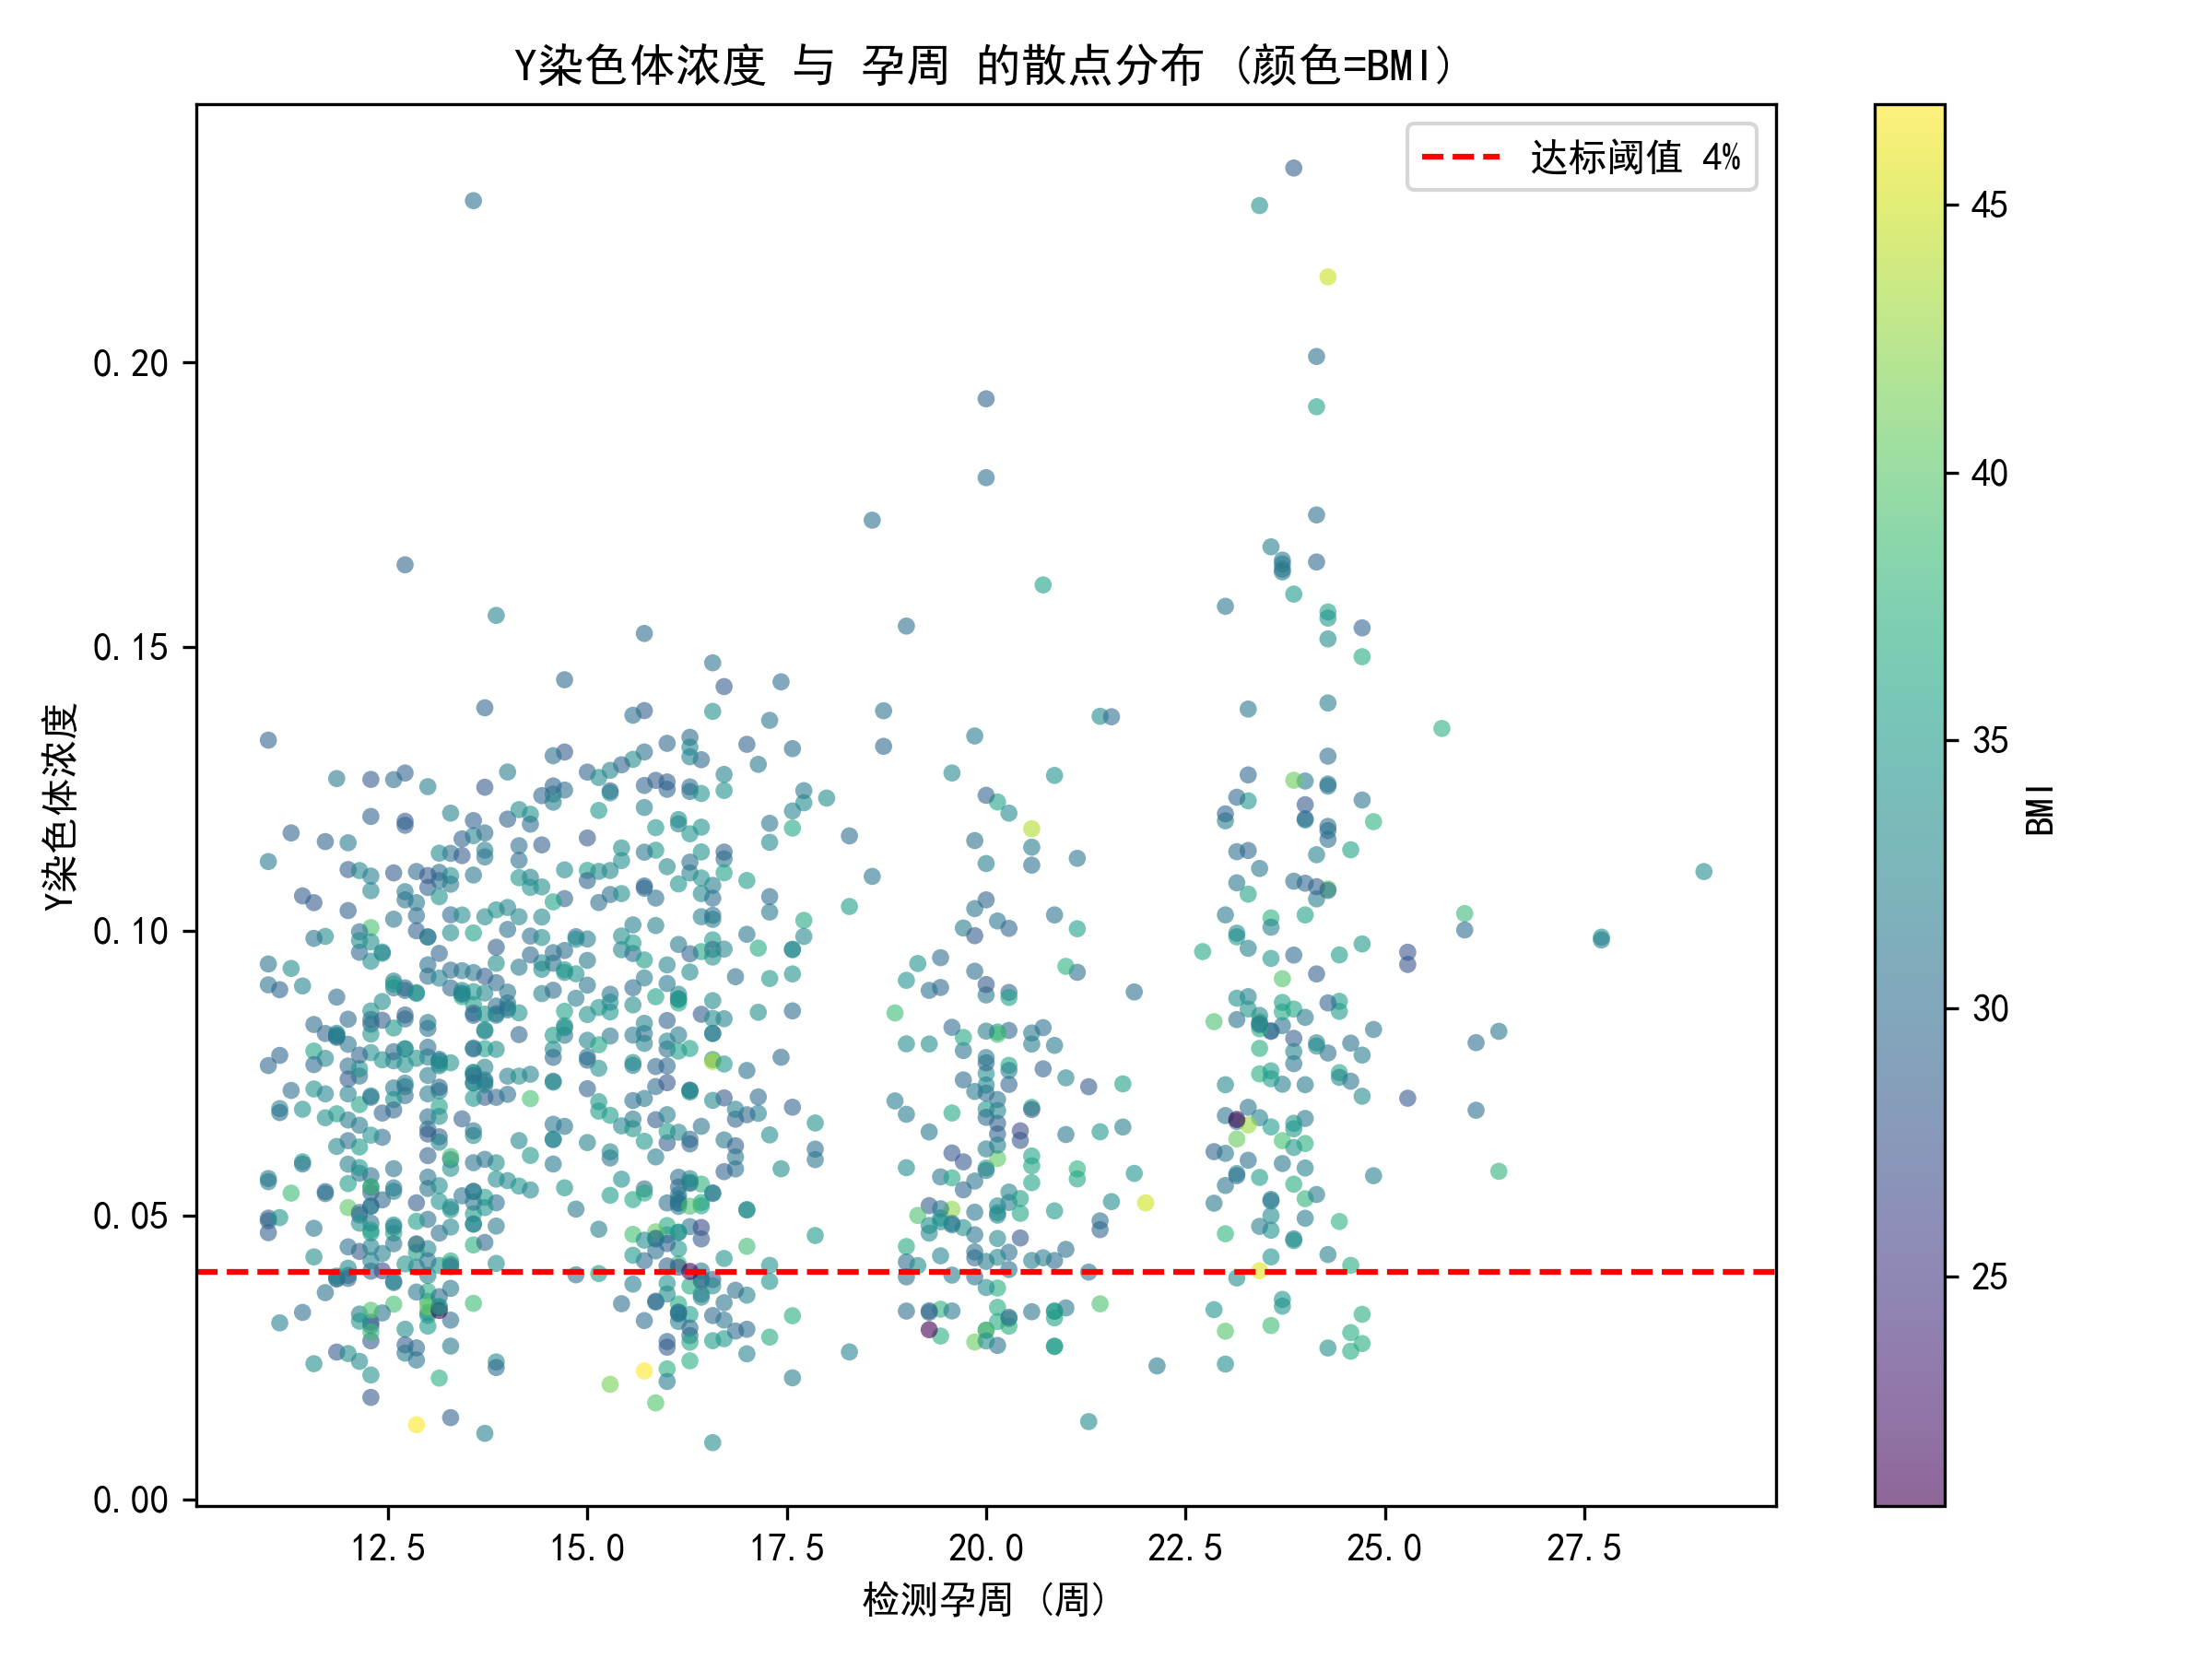
\includegraphics[width=0.75\textwidth]{output/figures/fig1_Y浓度_孕周_散点.png}
\caption{Y染色体浓度与孕周的散点分布（颜色表示BMI，红虚线为4\%达标阈值）}
\label{fig:scatter}
\end{figure}

\begin{figure}[H]
\centering
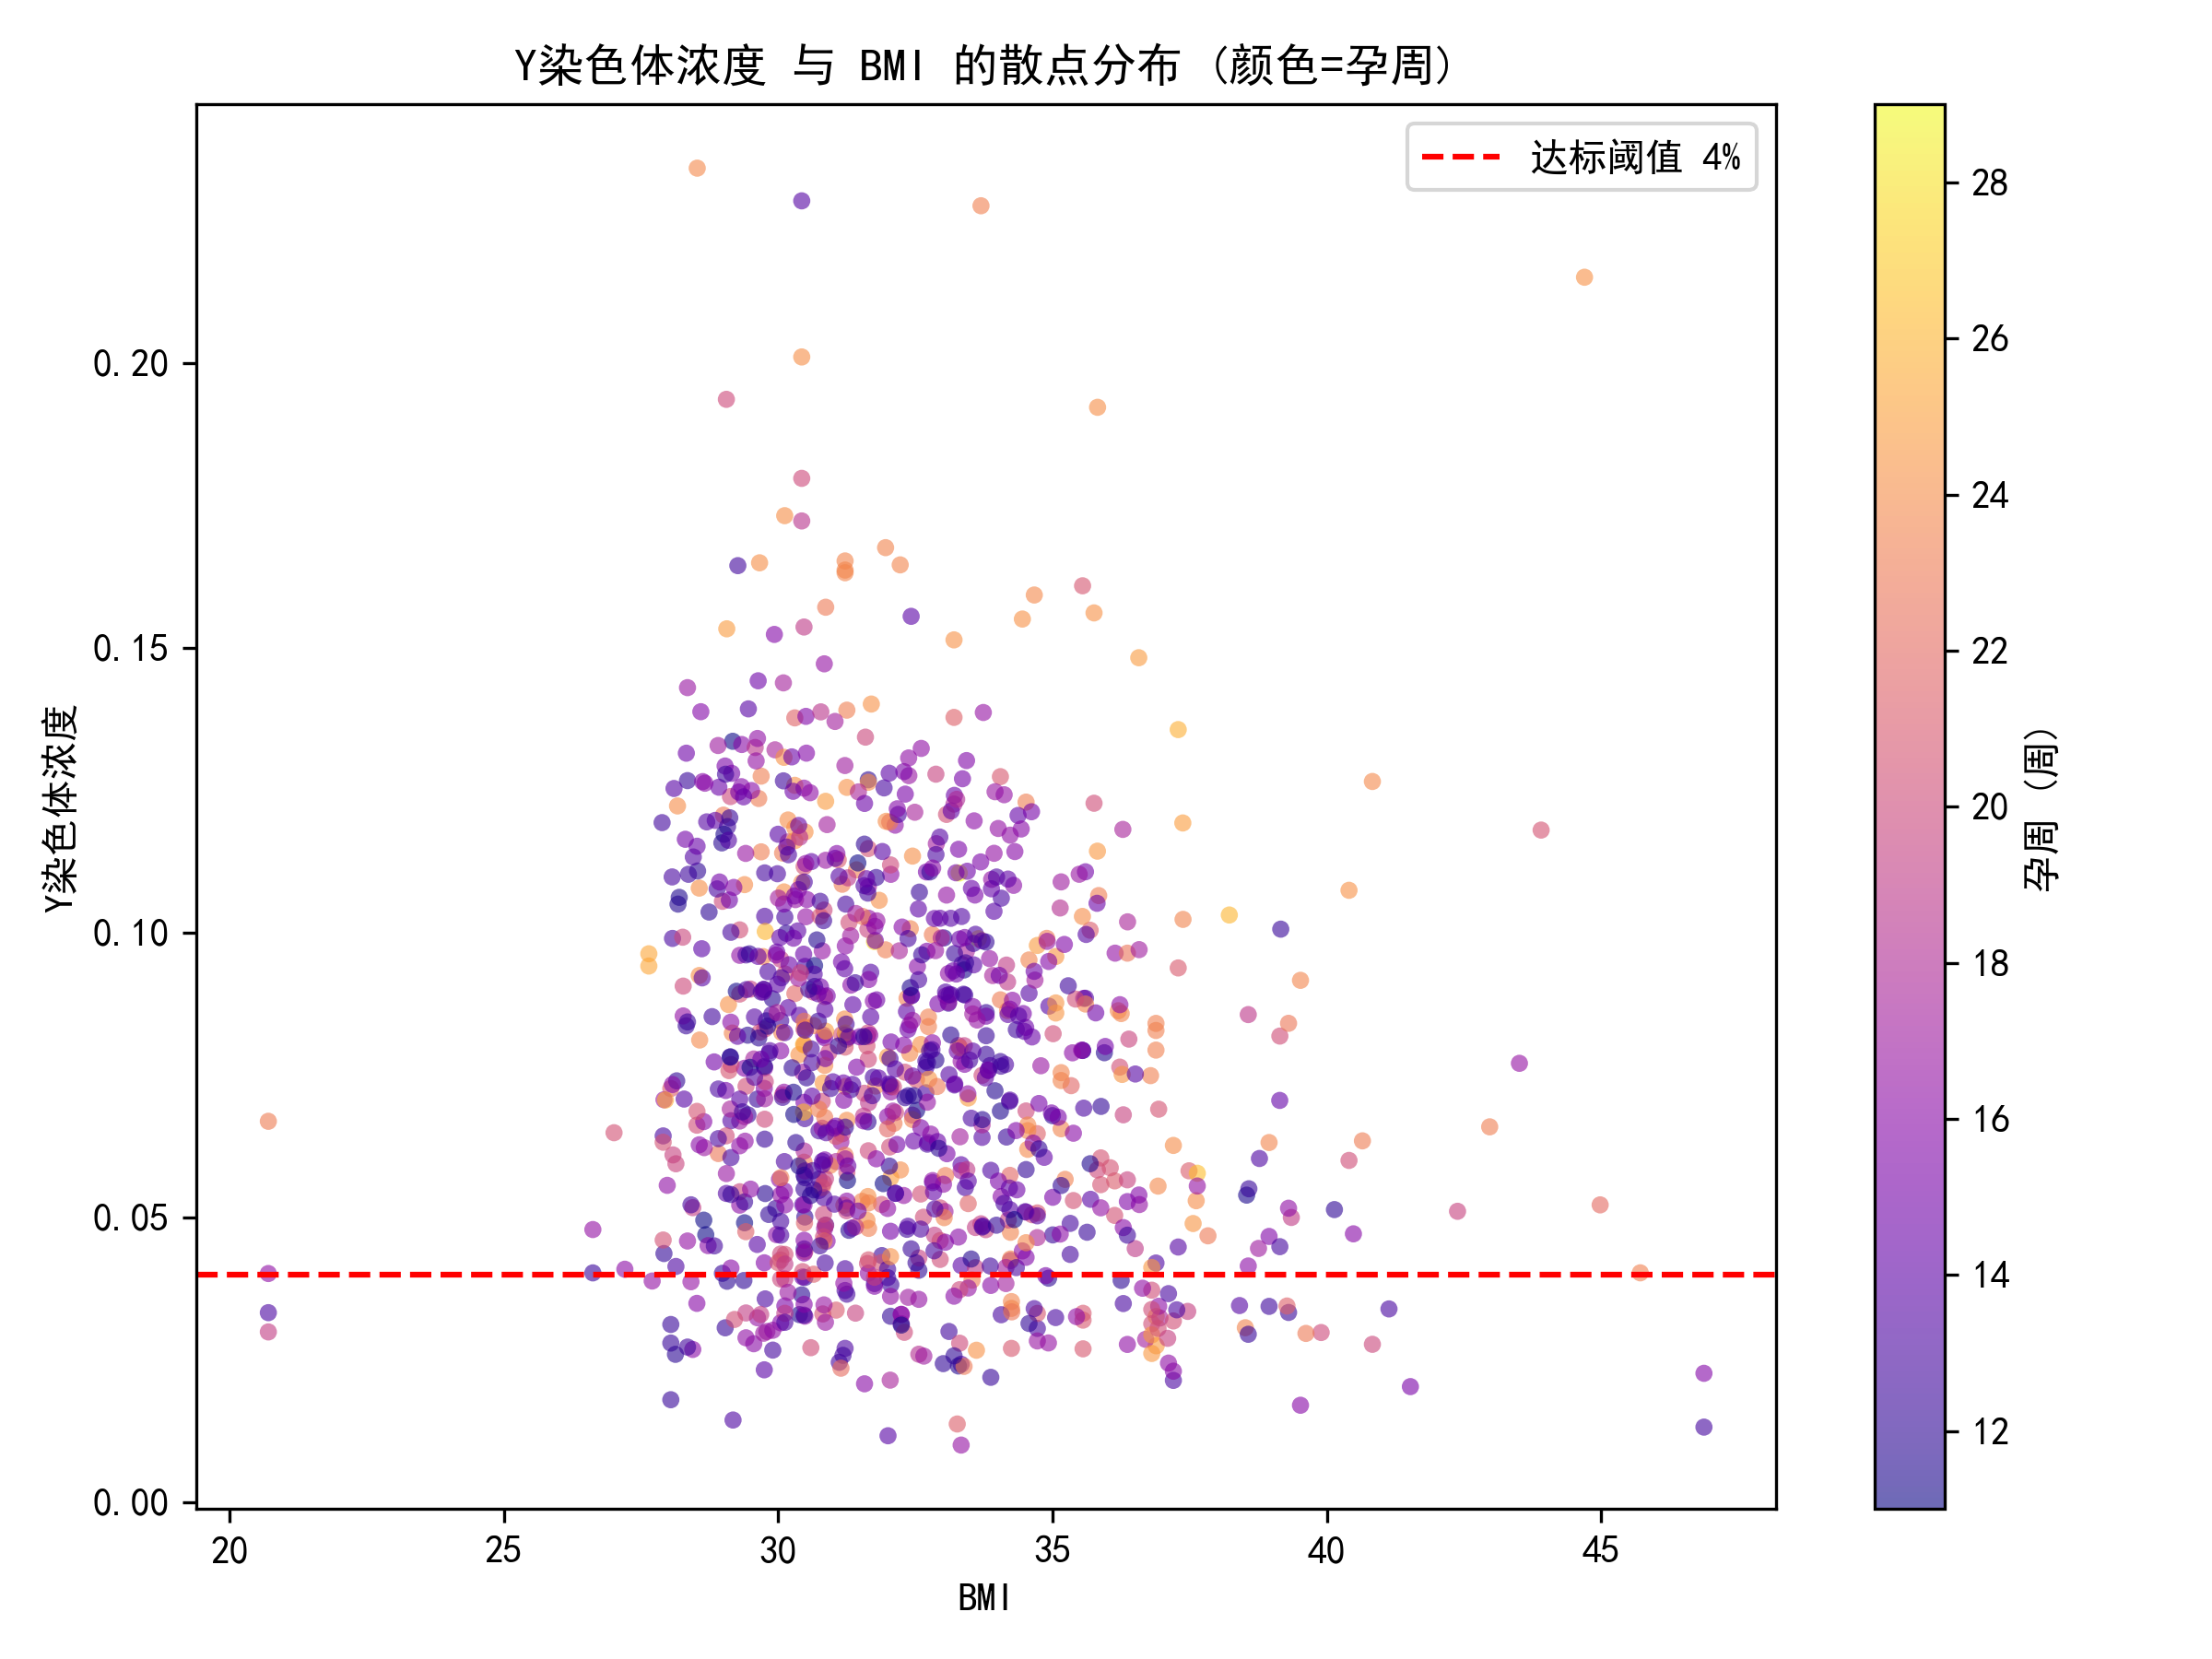
\includegraphics[width=0.75\textwidth]{output/figures/fig2_Y浓度_BMI_散点.png}
\caption{Y染色体浓度与BMI的散点分布（颜色表示孕周，红虚线为4\%达标阈值）}
\label{fig:bmi}
\end{figure}

\begin{figure}[H]
\centering
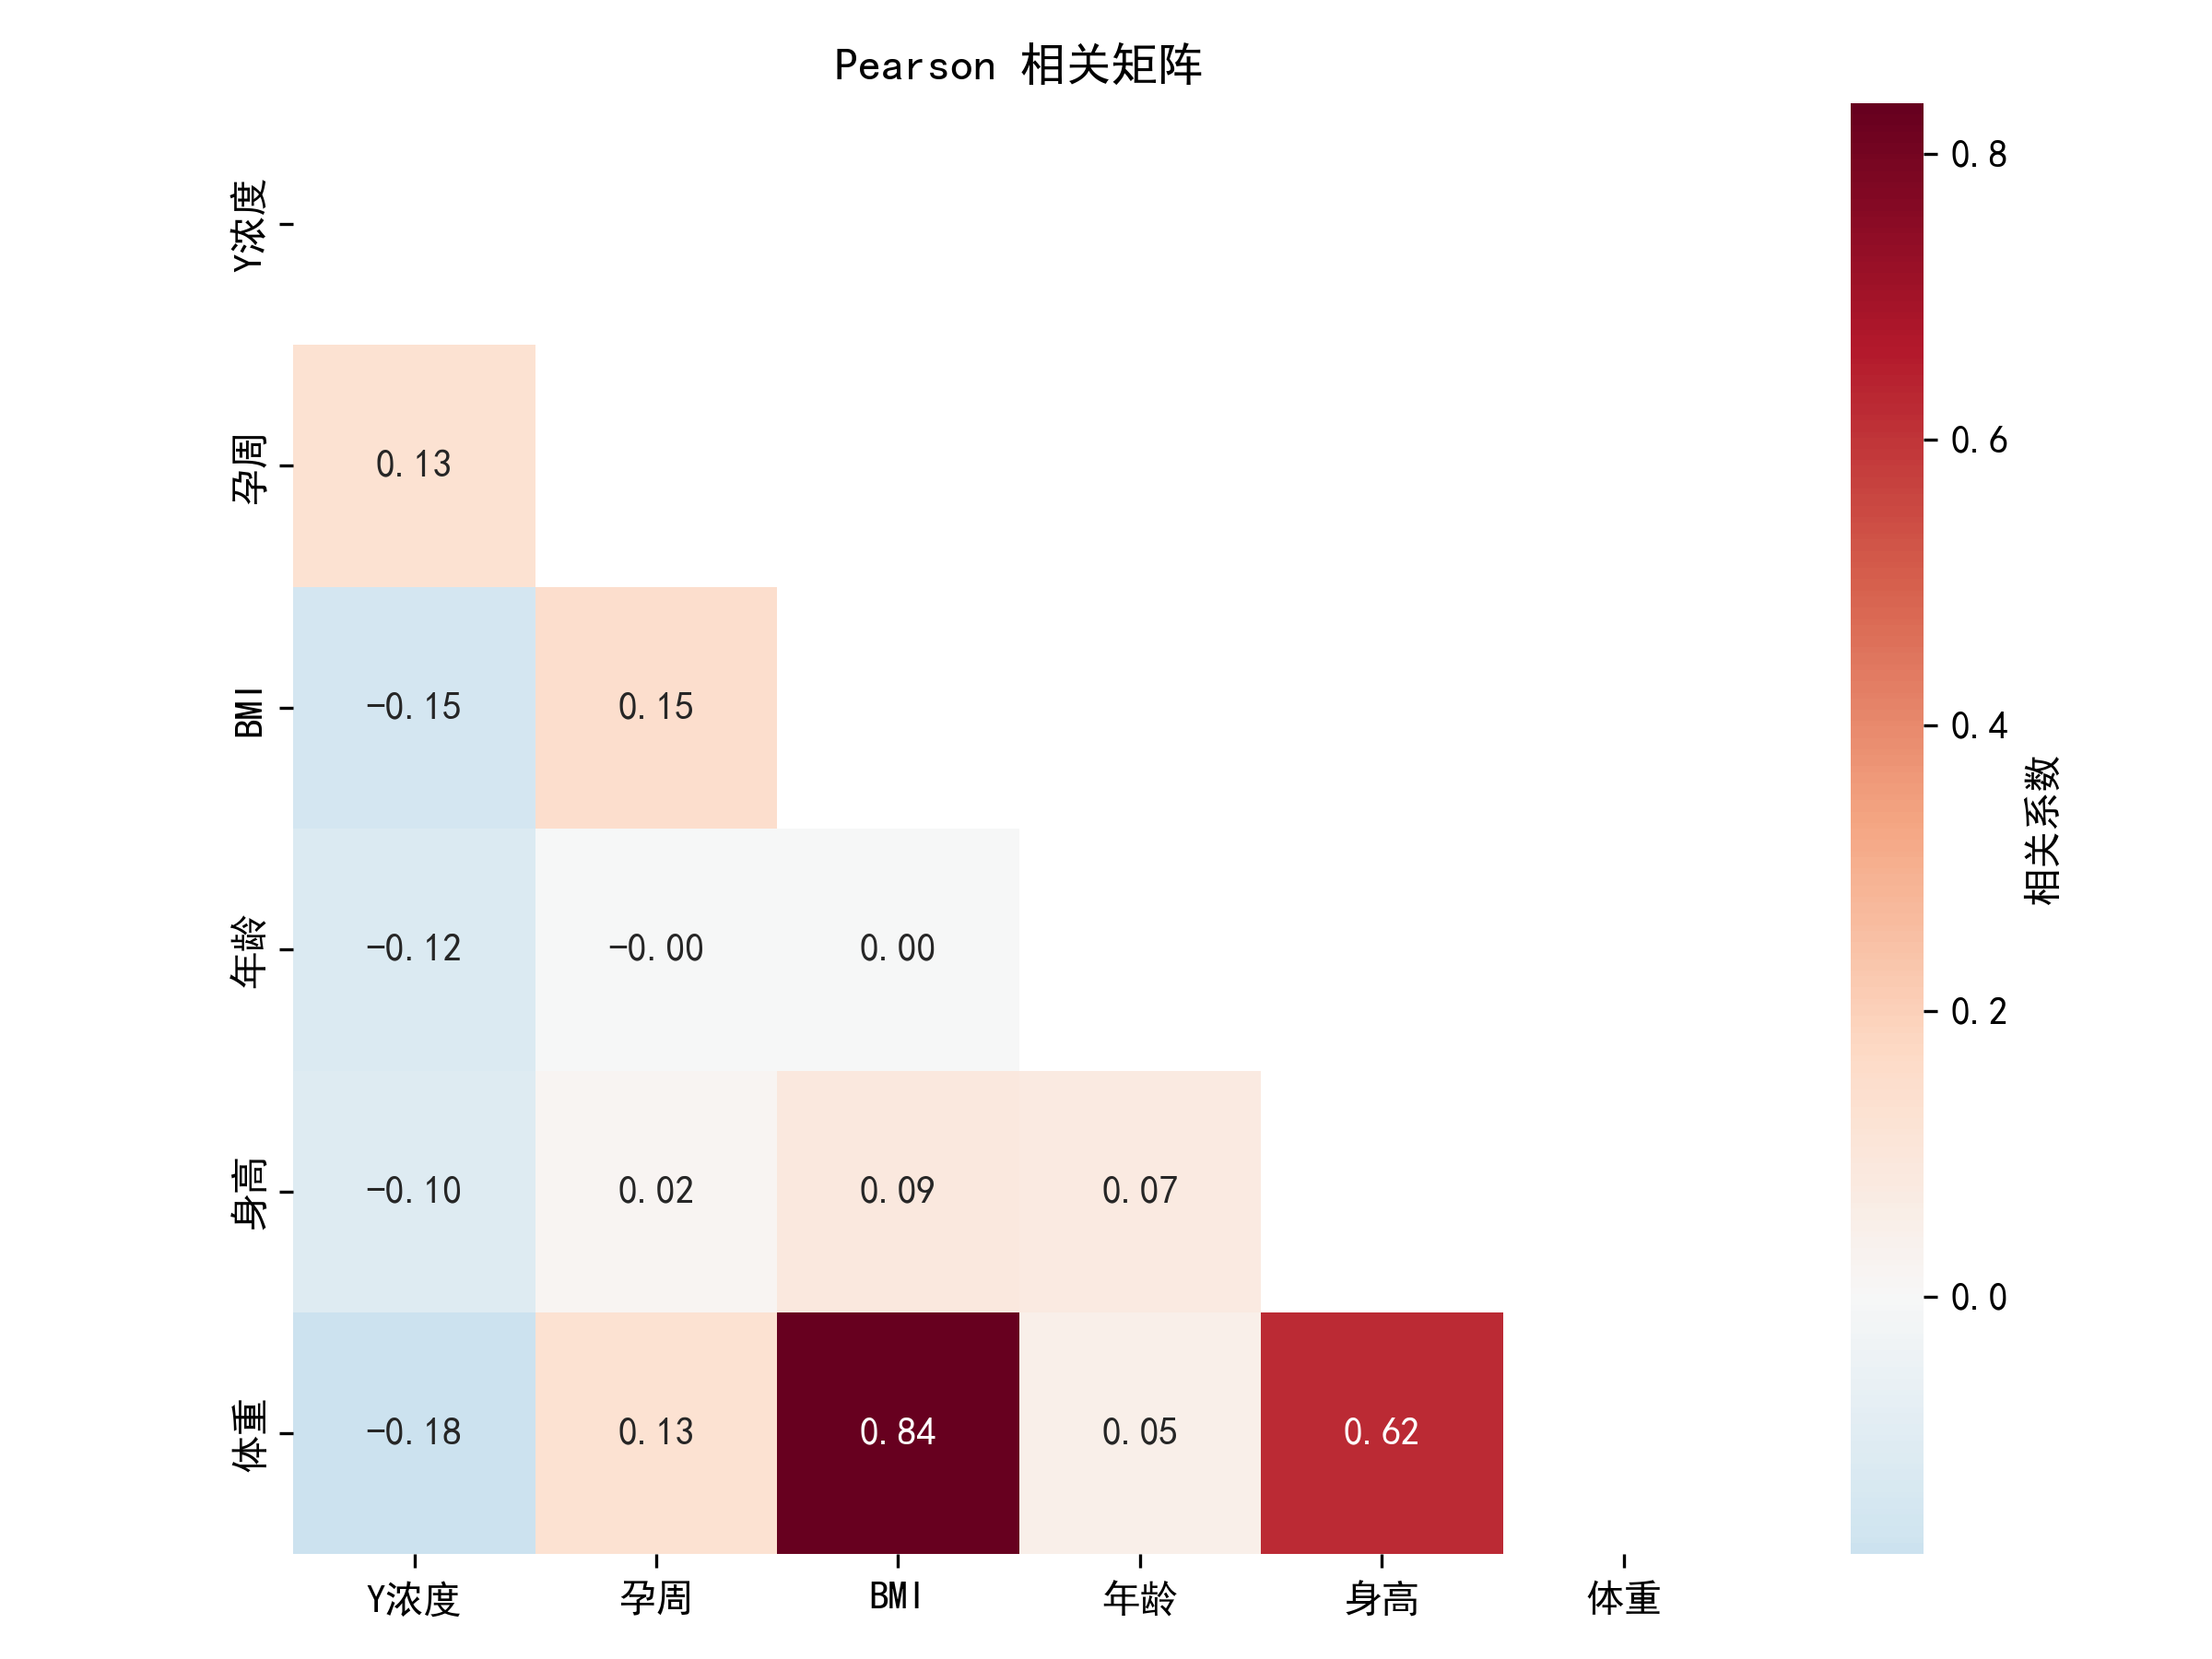
\includegraphics[width=0.72\textwidth]{output/figures/fig3_相关矩阵.png}
\caption{主要指标的Pearson相关矩阵热力图}
\label{fig:corrmat}
\end{figure}

\subsection{混合效应关系模型}

数据为纵向追踪结构，1082条记录来自267位孕妇。若用普通最小二乘（OLS）回归，重复测量不独立会导致标准误低估、系数偏倚。为此建立随机截距混合效应模型：
\begin{equation}
\ln Y_{ij} = \beta_0 + \beta_1 (t_{ij}-\bar t) + \beta_2 (\mathrm{BMI}_{ij}-\overline{\mathrm{BMI}}) + u_i + \varepsilon_{ij},
\end{equation}
其中$i$为孕妇、$j$为检测次数，$u_i\sim N(0,\sigma_u^2)$为个体随机效应，$\varepsilon_{ij}\sim N(0,\sigma_e^2)$为残差。自变量中心化以避免二次项与交互项共线。

模型估计结果见表\ref{tab:mixed}。混合效应模型中孕周系数为$0.044$（$z=18.7$，$p<0.001$），而横截面OLS的孕周系数仅$0.014$（$t=4.1$）。二者差异源于混杂：高BMI孕妇倾向于更晚检测，横截面回归将"个体差异"误并入孕周效应。个体间方差占比$\mathrm{ICC}=\sigma_u^2/(\sigma_u^2+\sigma_e^2)=72.6\%$，表明七成以上的变异来自孕妇个体差异，印证了采用混合效应模型的必要性。图\ref{fig:group_trend}进一步展示了不同BMI组Y浓度随孕周的上升趋势，高BMI组的曲线整体更低，直观印证了BMI对浓度的负效应。

\begin{table}[H]
\centering
\caption{混合效应模型估计结果（因变量$\ln Y$）}
\label{tab:mixed}
\begin{tabular}{lrrrrr}
\toprule
项 & 估计值 & 标准误 & $z$ & $p$值 & 95\%置信区间 \\
\midrule
截距$\beta_0$ & $-2.653$ & 0.026 & $-102.3$ & $<0.001$ & $[-2.704,-2.602]$ \\
孕周$\beta_1$ & 0.044 & 0.002 & 18.7 & $<0.001$ & $[0.039,0.048]$ \\
BMI$\beta_2$ & $-0.021$ & 0.007 & $-2.79$ & 0.005 & $[-0.035,-0.006]$ \\
\midrule
个体方差$\sigma_u^2$ & 0.163 & --- & --- & --- & --- \\
残差方差$\sigma_e^2$ & 0.0615 & --- & --- & --- & --- \\
\bottomrule
\end{tabular}
\end{table}

\begin{figure}[H]
\centering
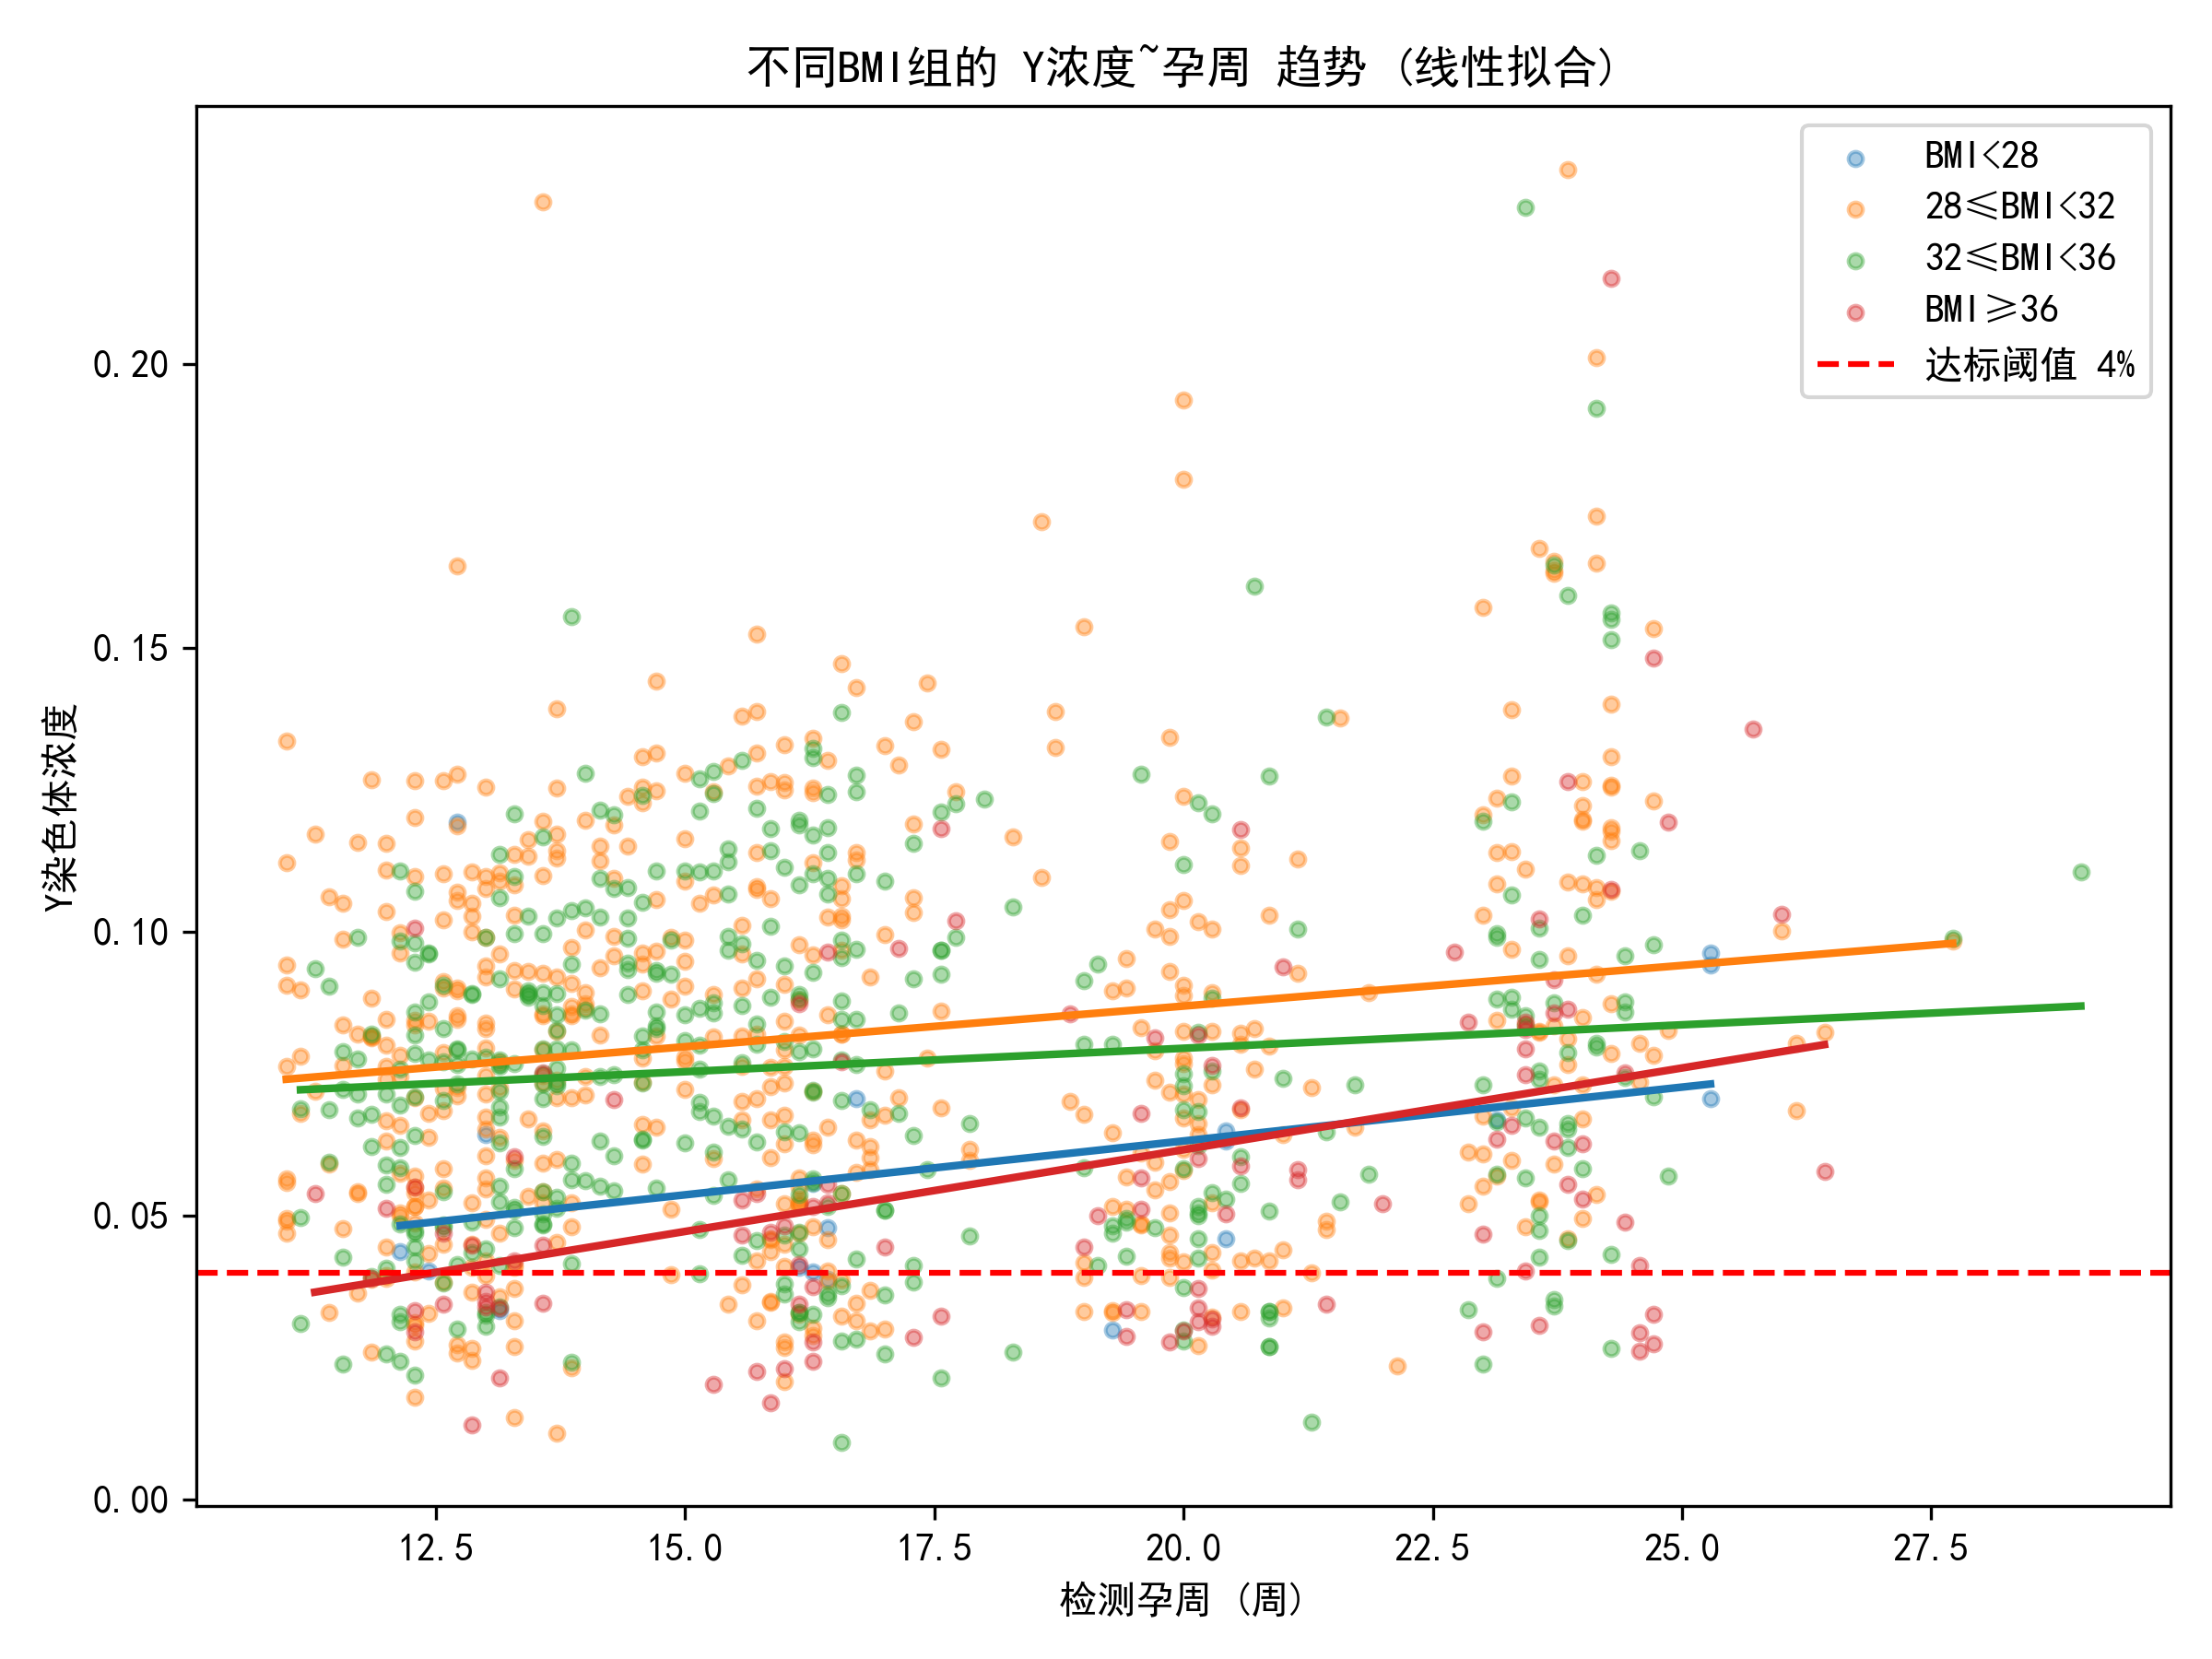
\includegraphics[width=0.85\textwidth]{output/figures/fig5_分BMI组趋势.png}
\caption{不同BMI组的Y浓度随孕周变化趋势（线性拟合，高BMI组整体更低）}
\label{fig:group_trend}
\end{figure}

\subsection{显著性检验}

对固定效应逐项做$t$检验：孕周与BMI的系数$p$值均小于$0.01$，整体模型高度显著。嵌套模型$F$检验显示，加入BMI后模型显著优于仅含孕周的模型（$F=24.76$，$p<0.001$）。残差诊断（图\ref{fig:resid}）表明残差近似正态、无显著异方差，模型设定合理。

\begin{figure}[H]
\centering
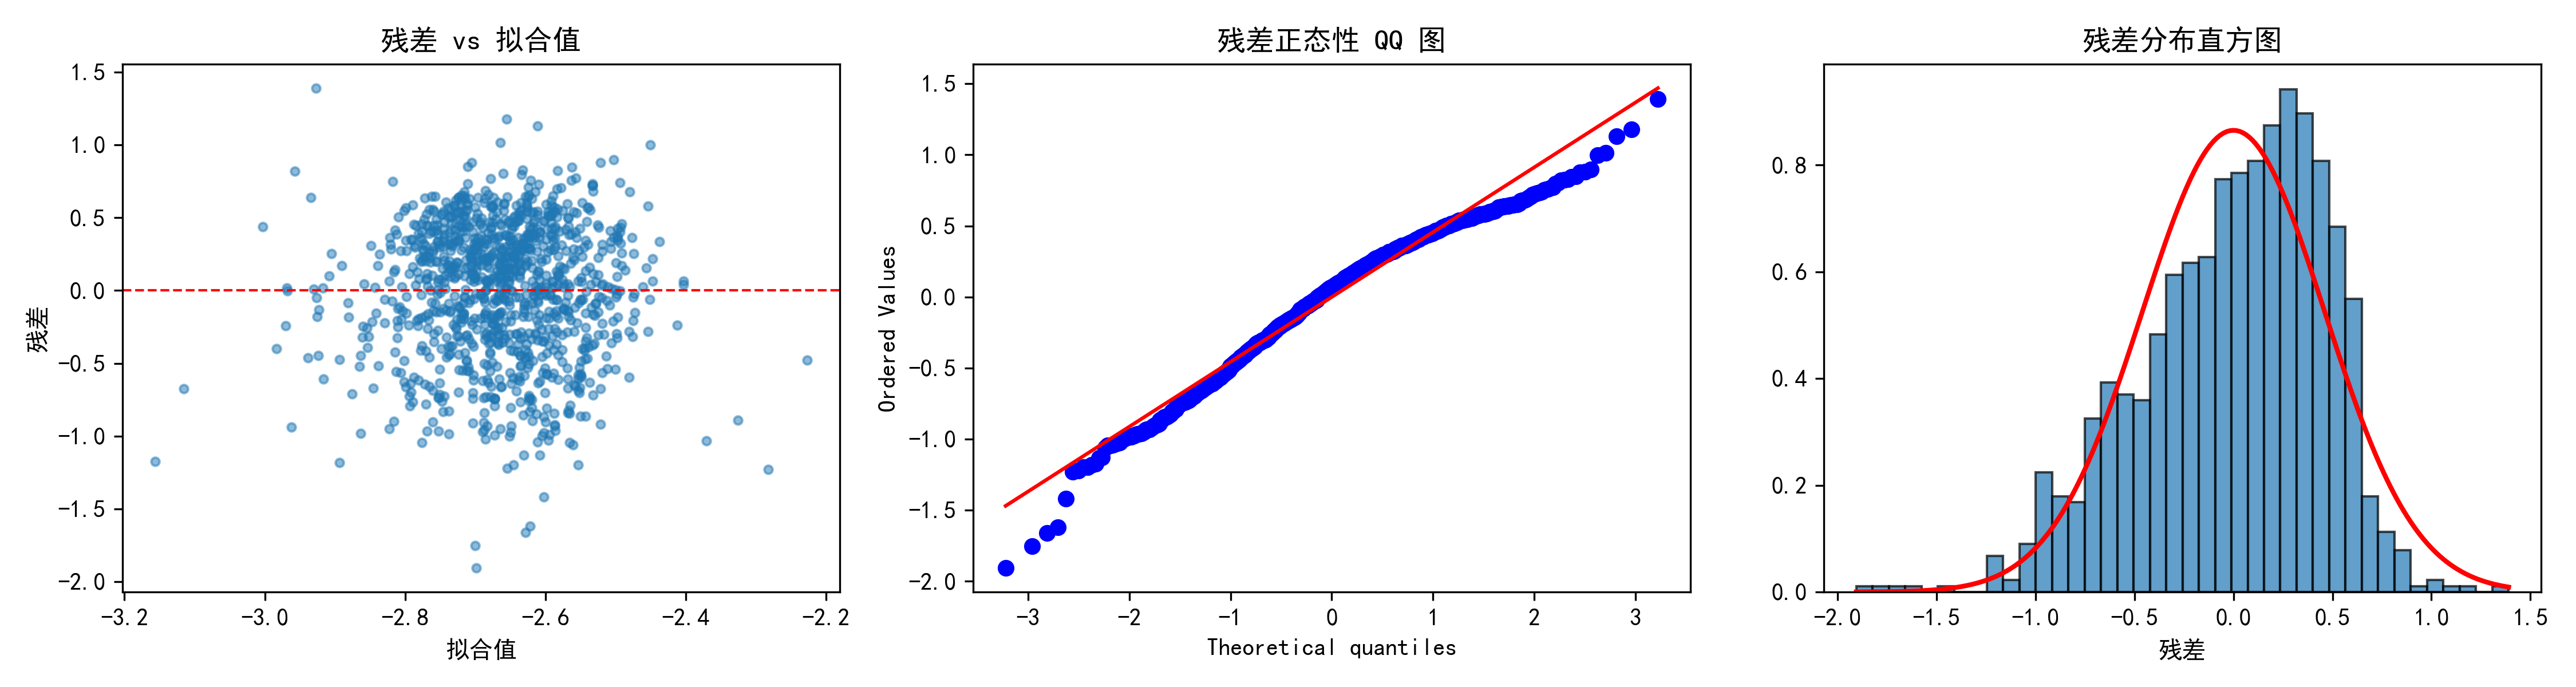
\includegraphics[width=0.95\textwidth]{output/figures/fig4_残差诊断.png}
\caption{问题一混合效应模型的残差诊断（残差-拟合图、QQ图、直方图）}
\label{fig:resid}
\end{figure}

进一步检验非线性效应。在混合效应框架下加入孕周与BMI的二次项，结果见表\ref{tab:quad}。孕周二次项高度显著（$p<0.001$，似然比检验$\chi^2=22.46$），BMI二次项不显著（$p=0.398$）。孕周二次项系数为正（$\hat\beta_3=0.00247$），反映Y浓度在孕周后段（$18\sim29$周）增长加速的生理规律。然而将二次模型用于达标时间外推时，在决策窗口（$10\sim16$周）内会产生无意义的预测（如G4组外推达标时间为$1.7$周），原因是孕周$10\sim14$周段样本稀疏、二次项在该段外推不可靠。故问题二、三仍采用线性模型，作为决策窗口内的稳健近似，与模型假设“对数浓度在检测窗口内线性相关”一致。

\begin{table}[H]
\centering
\caption{混合效应模型的二次项检验（ML估计）}
\label{tab:quad}
\begin{tabular}{lrr}
\toprule
模型 & AIC & 新增二次项$p$值 \\
\midrule
M0：week+BMI & 710.0 & --- \\
M1：+孕周$^2$ & 690.2 & $<0.001$ \\
M2：+BMI$^2$ & 711.4 & 0.398 \\
\bottomrule
\end{tabular}
\end{table}

\section{问题二：BMI分组与最佳NIPT时点}

\subsection{潜在风险的量化}

检测时点$t$的潜在风险由两部分构成：检测过早导致的浓度不达标风险$1-F(t)$，以及检测过晚导致的延误风险$D(t)$。综合风险定义为
\begin{equation}
R(t) = \big(1-F(t)\big) + \rho\, D(t),
\end{equation}
其中$F(t)$为达标比例（$Y\ge4\%$的比例），$D(t)$为题设的三级延误风险（$t\le12$为低风险取$0$，$13\le t\le27$为高风险取$1$，$t\ge28$为极高风险取$3$），$\rho$为延误相对检测不准的权重。延误权重$\rho$与置信水平$\alpha$存在单调对应关系：$\alpha$越高、时点越晚，等价于$\rho$越小。由于$\alpha$具有明确的统计含义且便于标定，本文直接以$\alpha$作为风险权衡参数，而不凭经验设定$\rho$。

达标比例$F(t)$由混合效应模型预测分布给出。对给定BMI与孕周，$\ln Y$服从$N(\mu(t),\sigma^2)$，其中$\mu(t)=\beta_0+\beta_1(t-\bar t)+\beta_2(\mathrm{BMI}-\overline{\mathrm{BMI}})$为固定效应预测。这里须区分两种方差：以个体间方差$\sigma_u$刻画"真实达标比例"（生物学上的群体比例），以总方差$\sigma_{\rm total}=\sqrt{\sigma_u^2+\sigma_e^2}$刻画"测得达标比例"（含测量误差后实际可观测的比例）。二者的差异即量化了检测误差的影响。

\subsection{BMI分组}

依据中国成人肥胖临床分级并兼顾样本量，将BMI分为四组，见表\ref{tab:group}。组G1样本量仅19例，但其达标时间由全部1082条记录估计的全局固定效应给出，不依赖组内拟合，故不受小样本影响。

\begin{table}[H]
\centering
\caption{BMI分组及样本量}
\label{tab:group}
\begin{tabular}{lrrr}
\toprule
分组 & BMI区间 & 样本量 & BMI范围 \\
\midrule
G1 & $<28$ & 19 & $[20.7,28.0]$ \\
G2 & $28\sim32$ & 539 & $[28.0,32.0]$ \\
G3 & $32\sim36$ & 413 & $[32.0,36.0]$ \\
G4 & $\ge36$ & 111 & $[36.1,46.9]$ \\
\bottomrule
\end{tabular}
\end{table}

\subsection{最佳时点的确定}

达标时间$t^*$满足$\mu(t^*) - z_\alpha\sigma = \ln 0.04$，即达标比例达到置信水平$\alpha$的最早孕周。置信水平的选择需权衡：$95\%$过于保守导致时点过晚（$18\sim25$周），$50\%$过于宽松导致时点过早（不足10周）。本文取$80\%$作为最佳时点的判定标准，理由有三：其一，经济与临床意义上，80\%达标意味着每5人中4人一次检测即可达标，其余复测，这一比例在临床可接受；其二，统计上80\%处于"过保守"与"过宽松"之间；其三，80\%给出的时点$10\sim16$周与NIPT临床常规检测窗口（12--16周）吻合。为进一步量化该选择，对$\alpha$在$60\%\sim95\%$间扫描，结果见表\ref{tab:alpha}与图\ref{fig:alpha}。

\begin{table}[H]
\centering
\caption{不同置信水平$\alpha$下的各组最佳时点（单位：周）}
\label{tab:alpha}
\begin{tabular}{lrrrr}
\toprule
置信水平$\alpha$ & G1 & G2 & G3 & G4 \\
\midrule
60\% & 3.6 & 5.5 & 7.4 & 9.3 \\
70\% & 6.6 & 8.5 & 10.4 & 12.3 \\
80\% & 10.0 & 11.9 & 13.8 & 15.7 \\
90\% & 14.8 & 16.7 & 18.6 & 20.5 \\
95\% & 18.8 & 20.7 & 22.6 & 24.5 \\
\bottomrule
\end{tabular}
\end{table}

\begin{figure}[H]
\centering
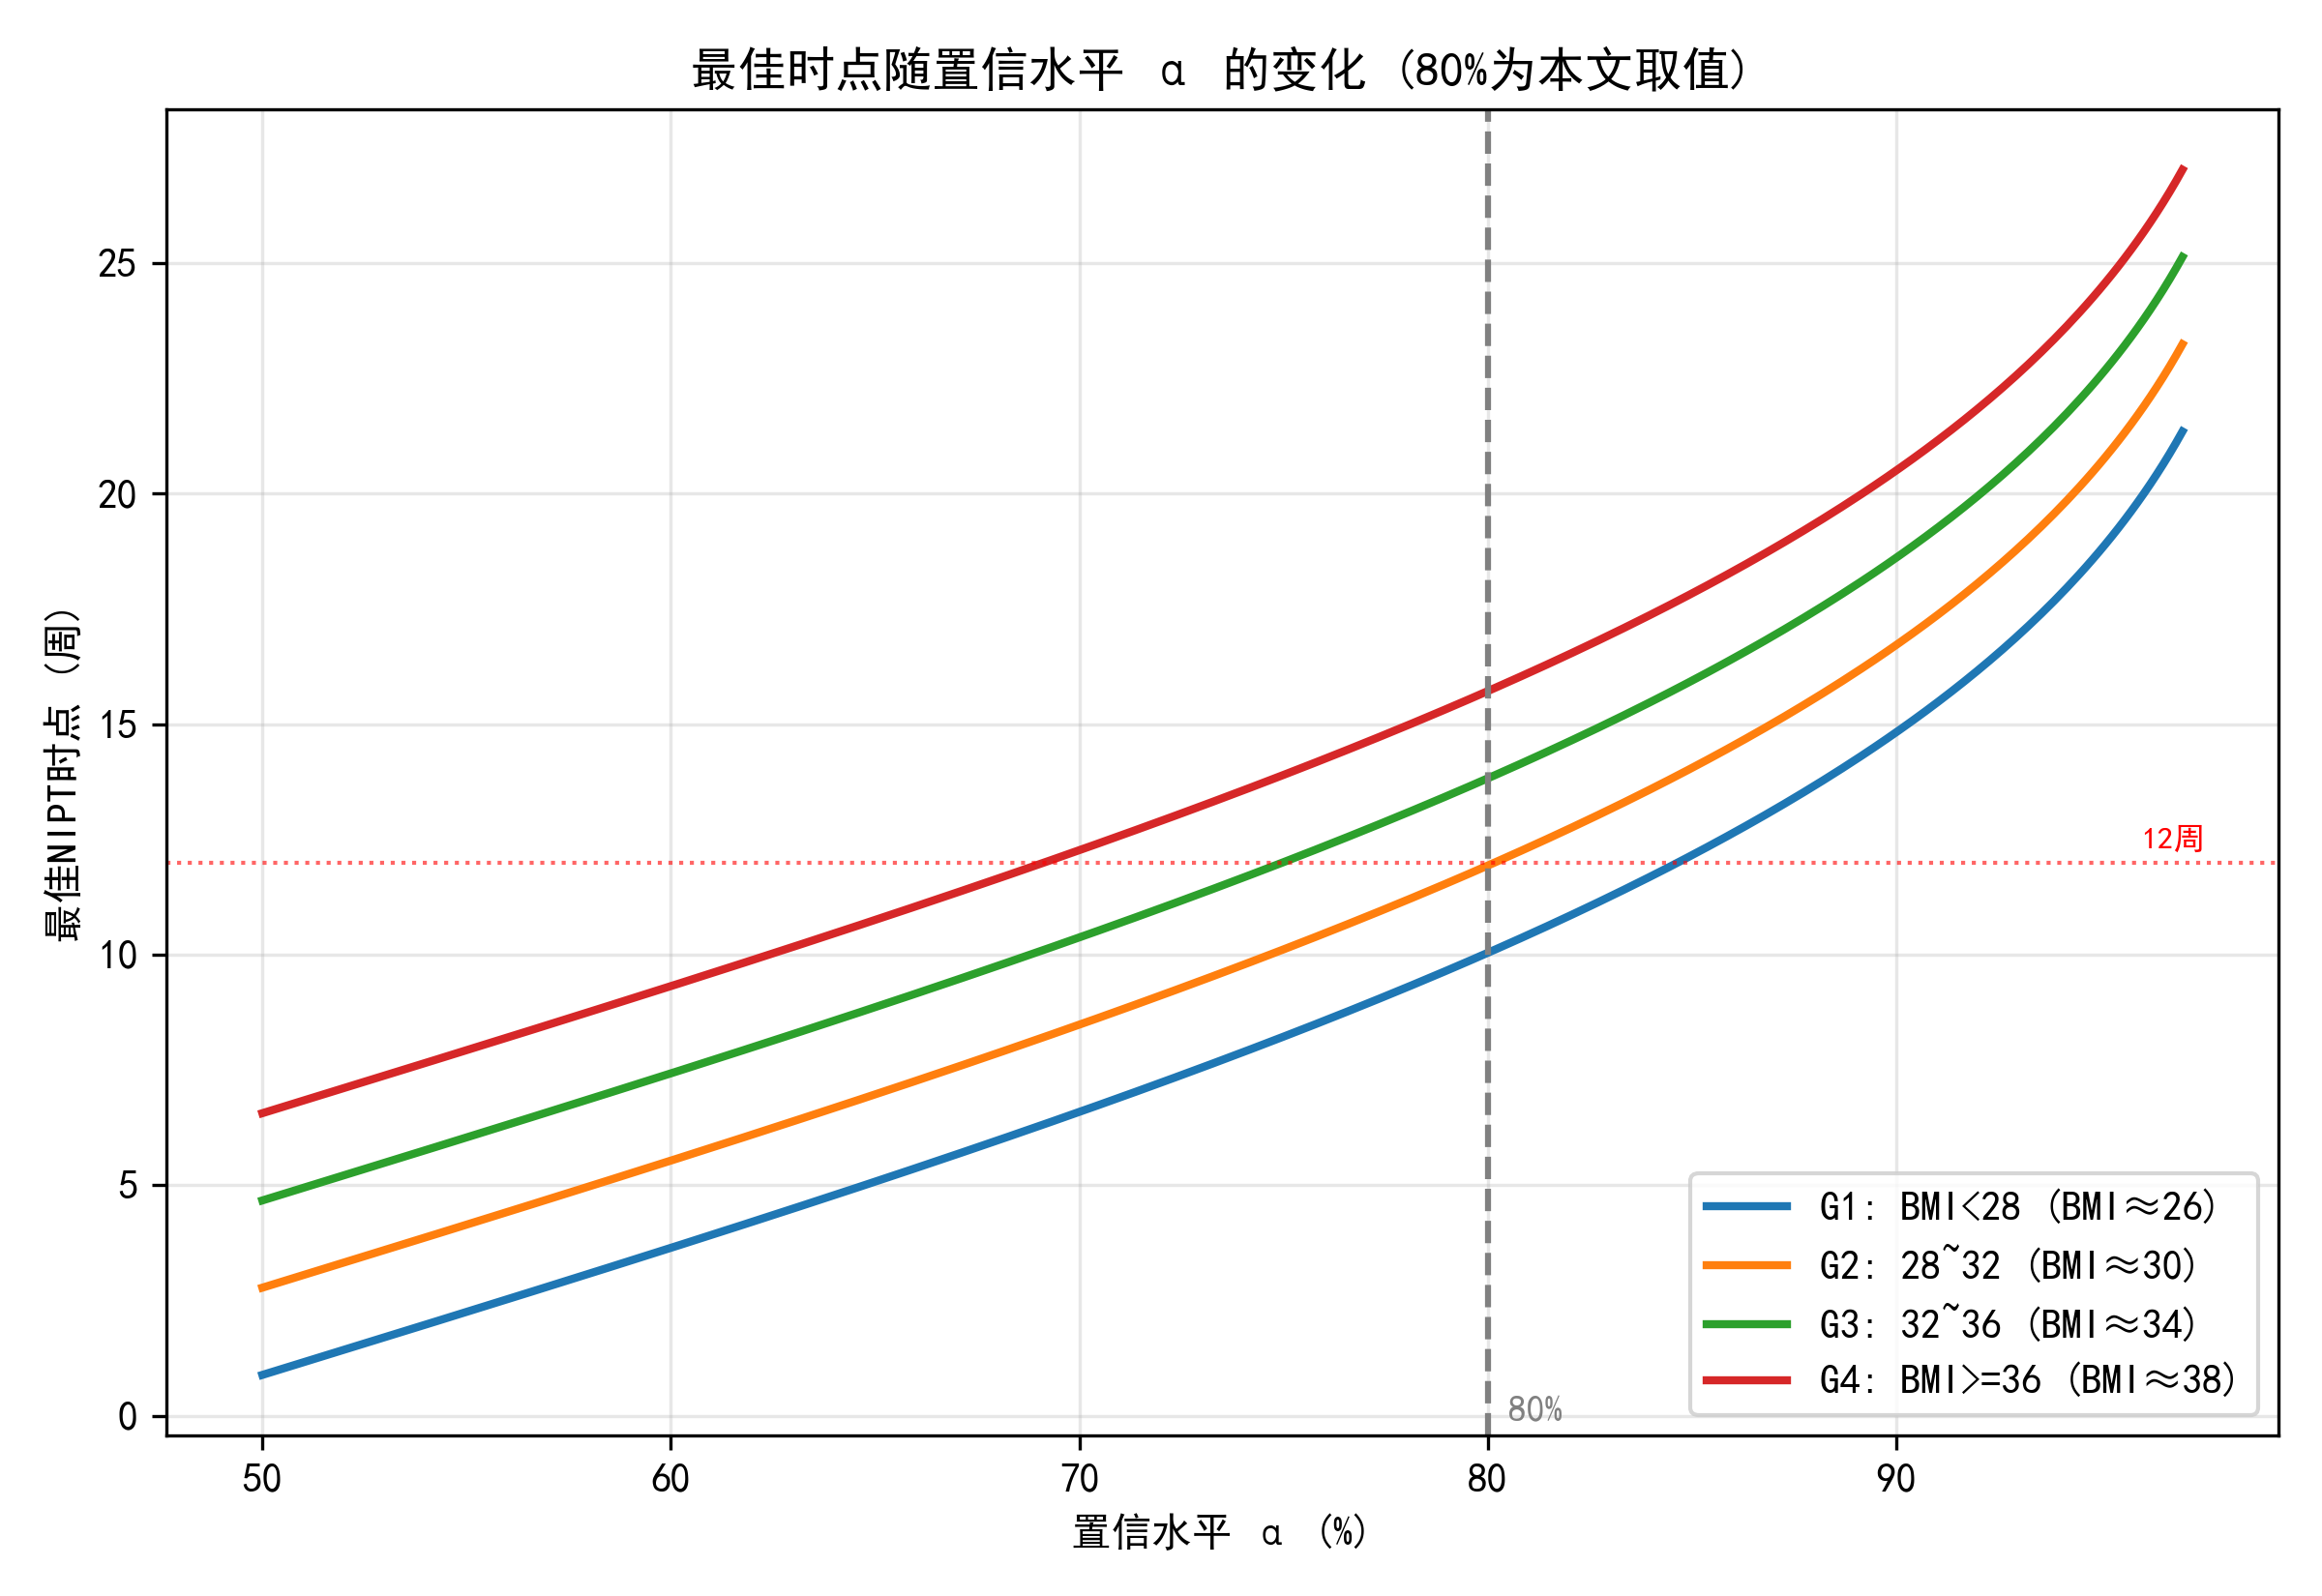
\includegraphics[width=0.85\textwidth]{output/figures/fig_supp_alpha扫描.png}
\caption{最佳时点随置信水平$\alpha$的变化（$80\%$为本文取值）}
\label{fig:alpha}
\end{figure}

由表\ref{tab:alpha}可见，$\alpha=70\%$时G1组时点仅$6.6$周、早于NIPT临床可行窗口（10周）；$\alpha=85\%$及以上时G2--G4组均已进入$13\sim27$周的高风险区间。唯有$\alpha=80\%$使G1、G2组落在低风险区（$\le12$周）、G3、G4组处于可接受区间，且各组时点均不早于10周，兼顾检测可靠性与干预及时性，从数值上印证了$80\%$阈值的选择。

各组最佳时点见表\ref{tab:p2}与图\ref{fig:p2bar}。可见最佳时点随BMI单调后移：低BMI组10.0周即可可靠检测，而高BMI组需等到15.7周，此时已进入13--27周的高风险区间，说明高BMI孕妇面临更大的延误风险。

值得说明的是，本文所得最佳时点（$10.0\sim15.7$周）明显早于基于生存分析的Kaplan-Meier方法（约$17\sim18$周）。二者差异源于对"达标"的定义不同：生存分析以"个体首次测得$Y\ge4\%$"作为事件时间，其达标中位时间天然偏晚，反映的是最后一批个体达标的时间；本文则以"群体达标比例达$80\%$"为标准，刻画的是绝大多数孕妇已能可靠检测的时点。从临床常规看，NIPT多在$12\sim16$周实施，本文结果与之吻合；若将时点推迟至$17\sim18$周，反而过度保守、缩短异常胎儿的干预窗口。此外，生存分析中时间惩罚函数的参数（如指数速率与风险权重）通常凭经验设定，对最优时点影响较大且缺乏论证；本文的$80\%$阈值则经经济、统计与临床三方面论证，稳健性更强。

\begin{table}[H]
\centering
\caption{各BMI组达标时间与最佳时点（单位：周）}
\label{tab:p2}
\begin{tabular}{lrrrrr}
\toprule
分组 & 测得80\% & 测得90\% & 真实90\% & 最佳时点 & 风险等级 \\
\midrule
G1（BMI$<28$） & 10.0 & 14.8 & 12.8 & 10.0 & 低 \\
G2（$28\sim32$） & 11.9 & 16.7 & 14.7 & 11.9 & 低 \\
G3（$32\sim36$） & 13.8 & 18.6 & 16.6 & 13.8 & 高 \\
G4（BMI$\ge36$） & 15.7 & 20.5 & 18.4 & 15.7 & 高 \\
\bottomrule
\end{tabular}
\end{table}

图\ref{fig:p2}展示了各组达标比例曲线与最佳时点，图\ref{fig:p2t}展示了达标时间随BMI的变化。

\begin{figure}[H]
\centering
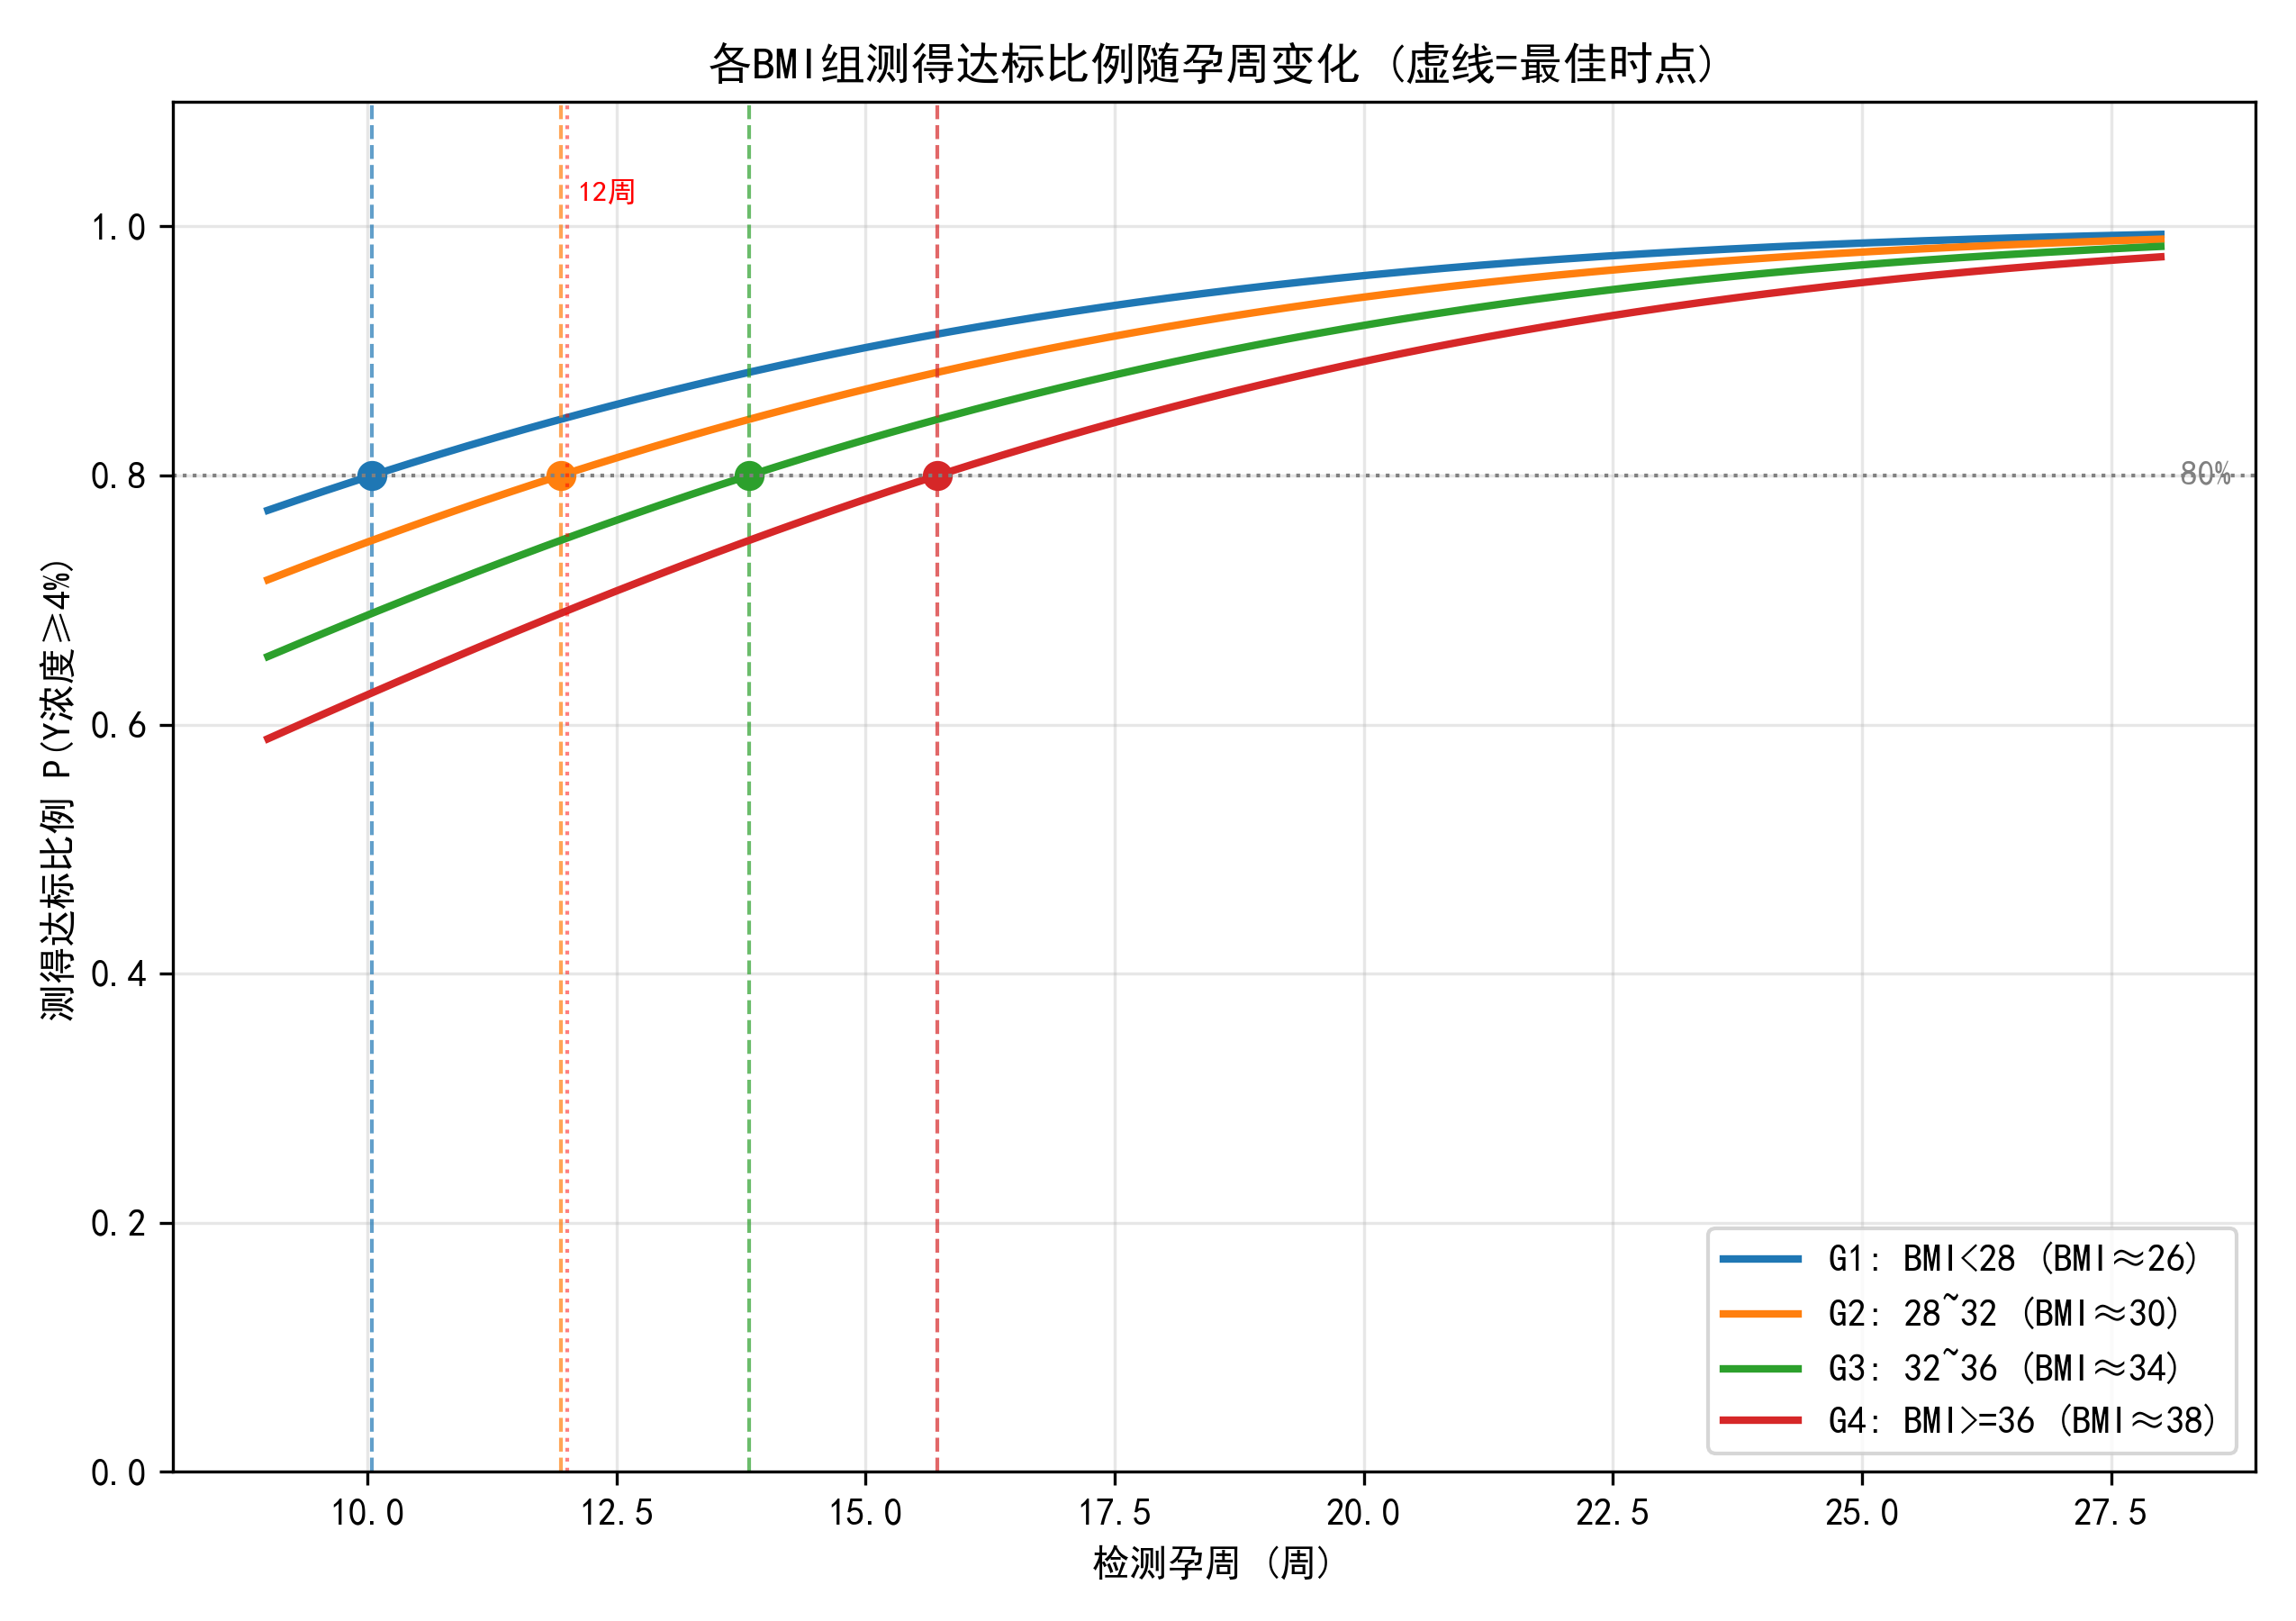
\includegraphics[width=0.85\textwidth]{output/figures/fig2-1_达标比例曲线.png}
\caption{各BMI组测得达标比例随孕周变化（虚线为最佳时点）}
\label{fig:p2}
\end{figure}

\begin{figure}[H]
\centering
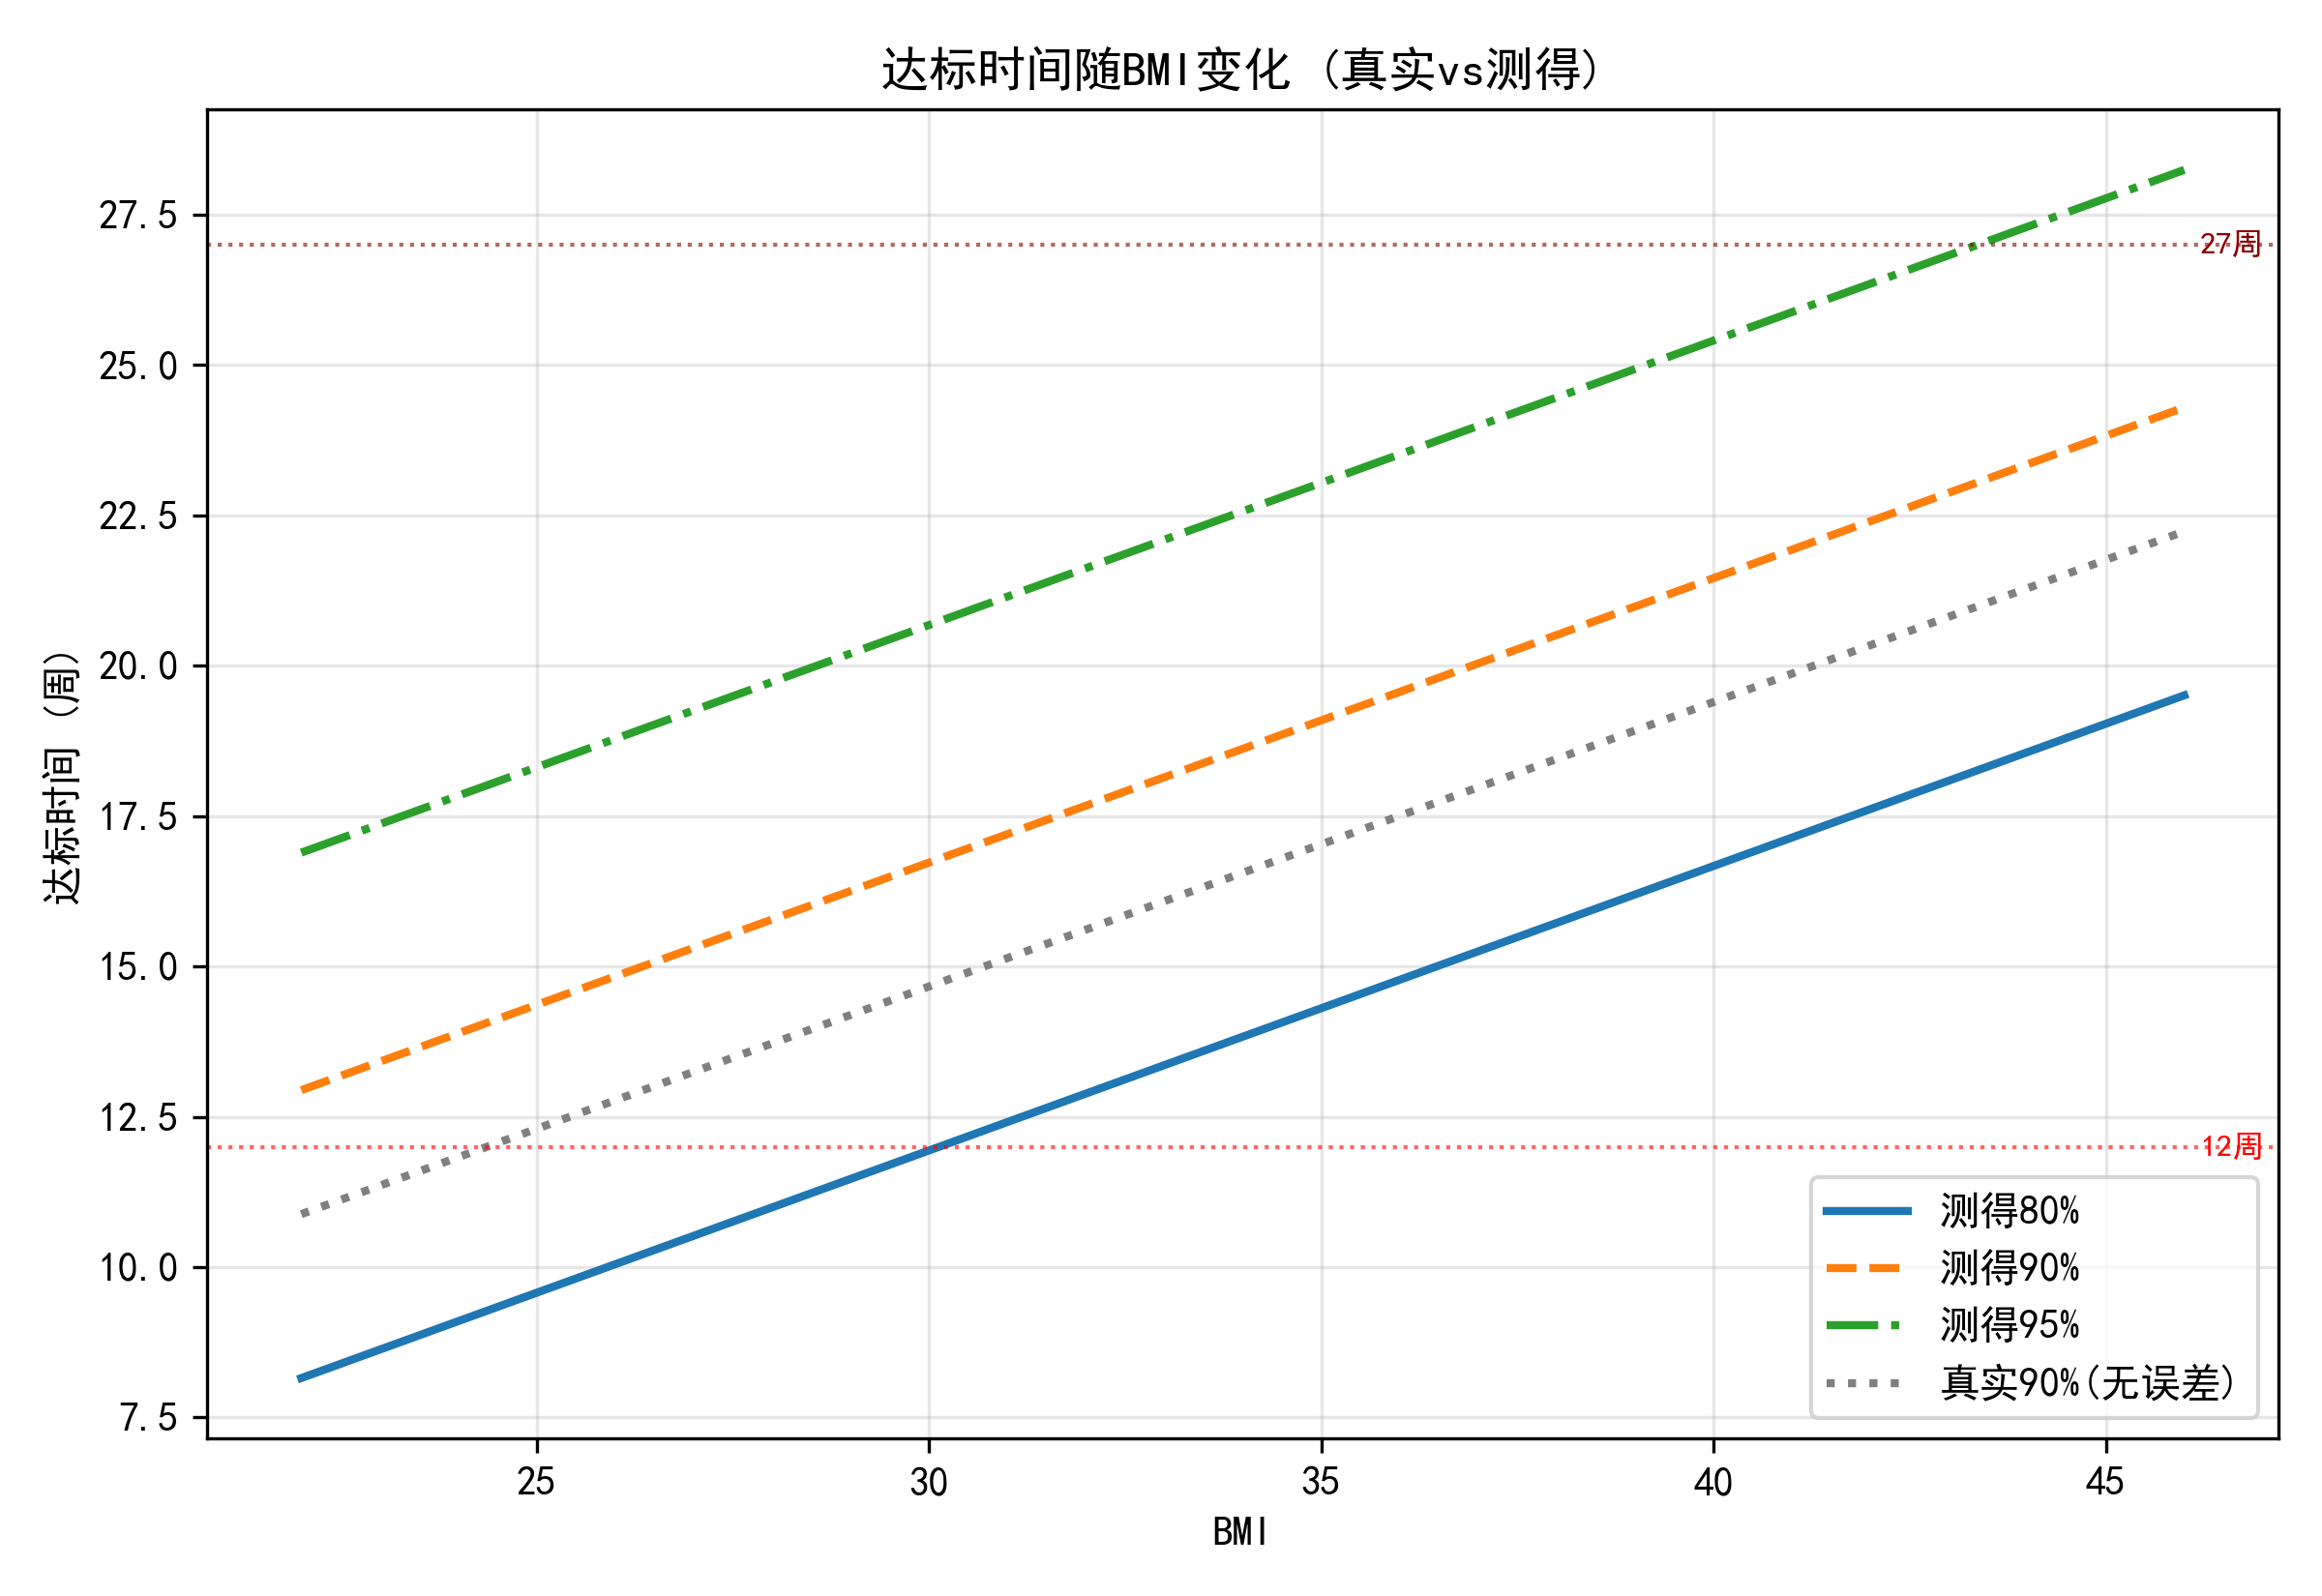
\includegraphics[width=0.85\textwidth]{output/figures/fig2-2_达标时间vsBMI.png}
\caption{达标时间随BMI的变化（真实达标与含误差的测得达标）}
\label{fig:p2t}
\end{figure}

\begin{figure}[H]
\centering
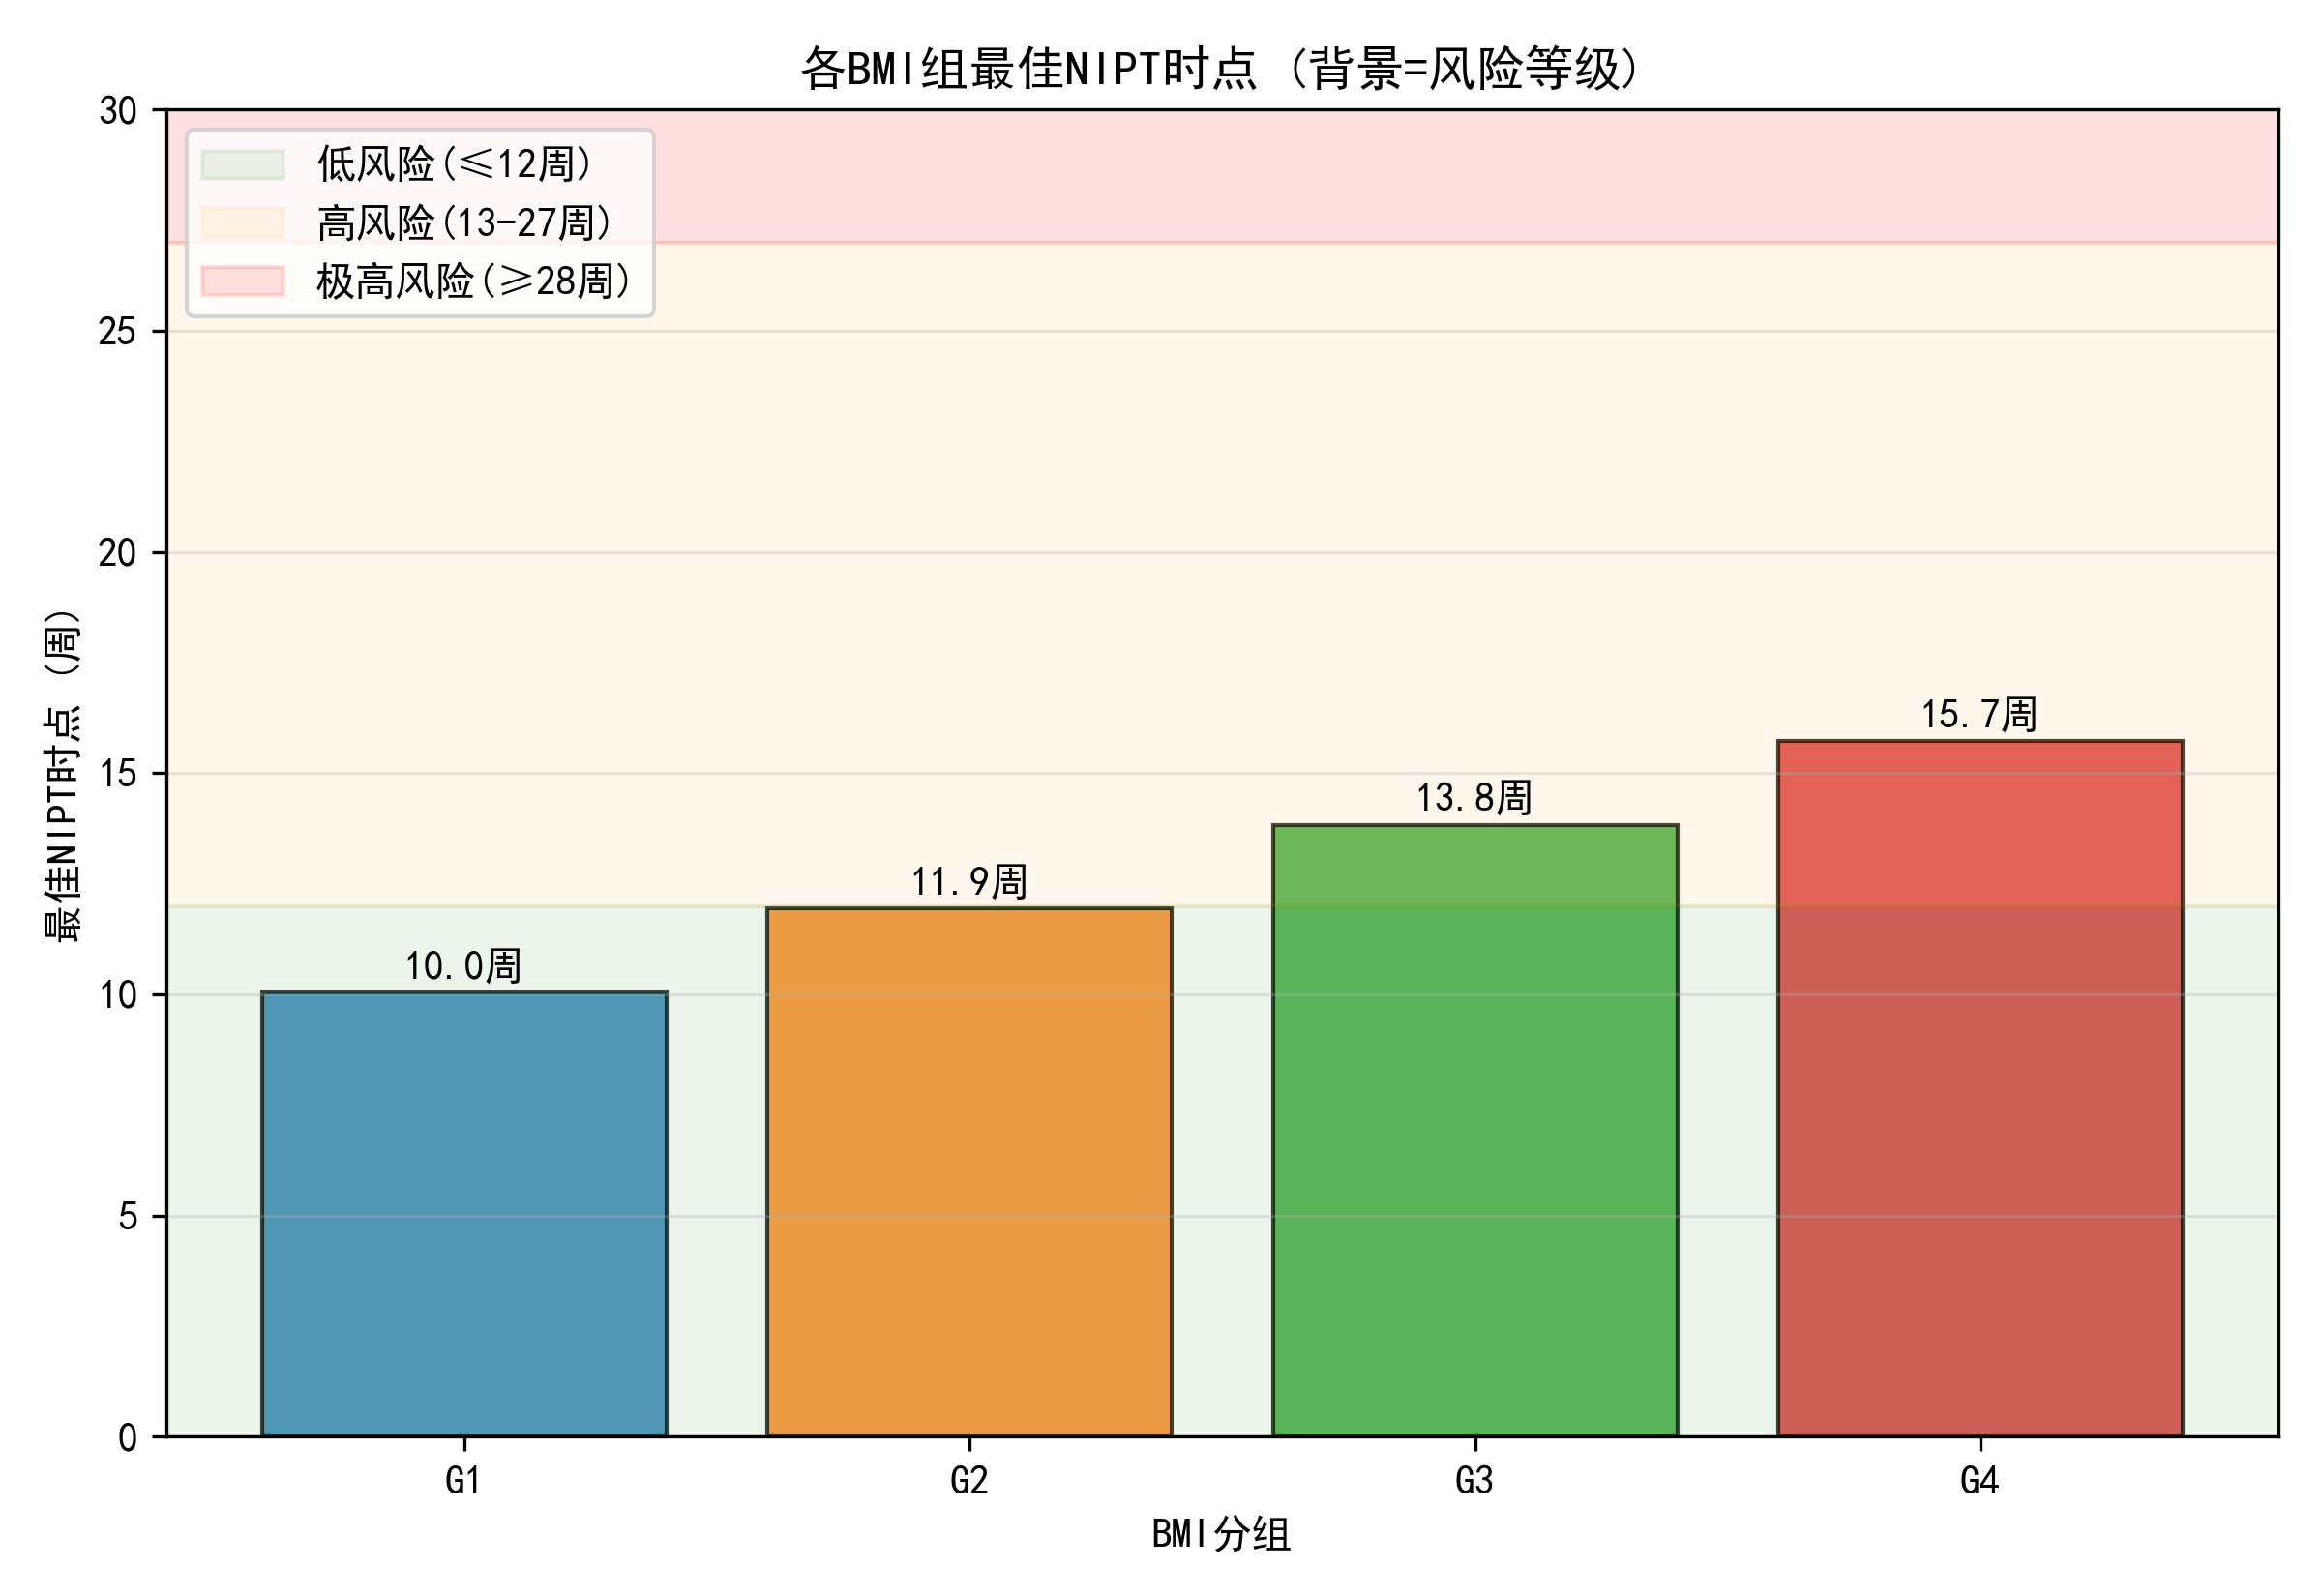
\includegraphics[width=0.8\textwidth]{output/figures/fig2-3_最佳时点柱状.png}
\caption{各BMI组最佳NIPT时点（背景色表示风险等级）}
\label{fig:p2bar}
\end{figure}

\subsection{检测误差的影响}

以90\%置信为例，测得达标时间与真实达标时间的差即为测量误差$\sigma_e$导致的达标时间推迟。由表\ref{tab:p2}，各组的测得90\%与真实90\%之差均为$2.06$周，即检测误差平均使达标时间推迟2.06周。进一步的聚类bootstrap（对孕妇有放回抽样200次，保持同一孕妇的记录成组）给出最佳时点的分布，见表\ref{tab:boot}。各组时点的不确定性约$\pm1$周，且组间差异显著，结论稳健，各组最佳时点的bootstrap分布见图\ref{fig:p2boot}。

\begin{table}[H]
\centering
\caption{聚类bootstrap下各组最佳时点的不确定性（B=200）}
\label{tab:boot}
\begin{tabular}{lrrr}
\toprule
分组 & 时点均值（周） & 标准差 & 95\%置信区间 \\
\midrule
G1（BMI$<28$） & 9.98 & 1.249 & $[7.4,12.1]$ \\
G2（$28\sim32$） & 11.93 & 0.795 & $[10.3,13.5]$ \\
G3（$32\sim36$） & 13.88 & 0.770 & $[12.5,15.4]$ \\
G4（BMI$\ge36$） & 15.84 & 1.201 & $[13.4,18.1]$ \\
\bottomrule
\end{tabular}
\end{table}

\begin{figure}[H]
\centering
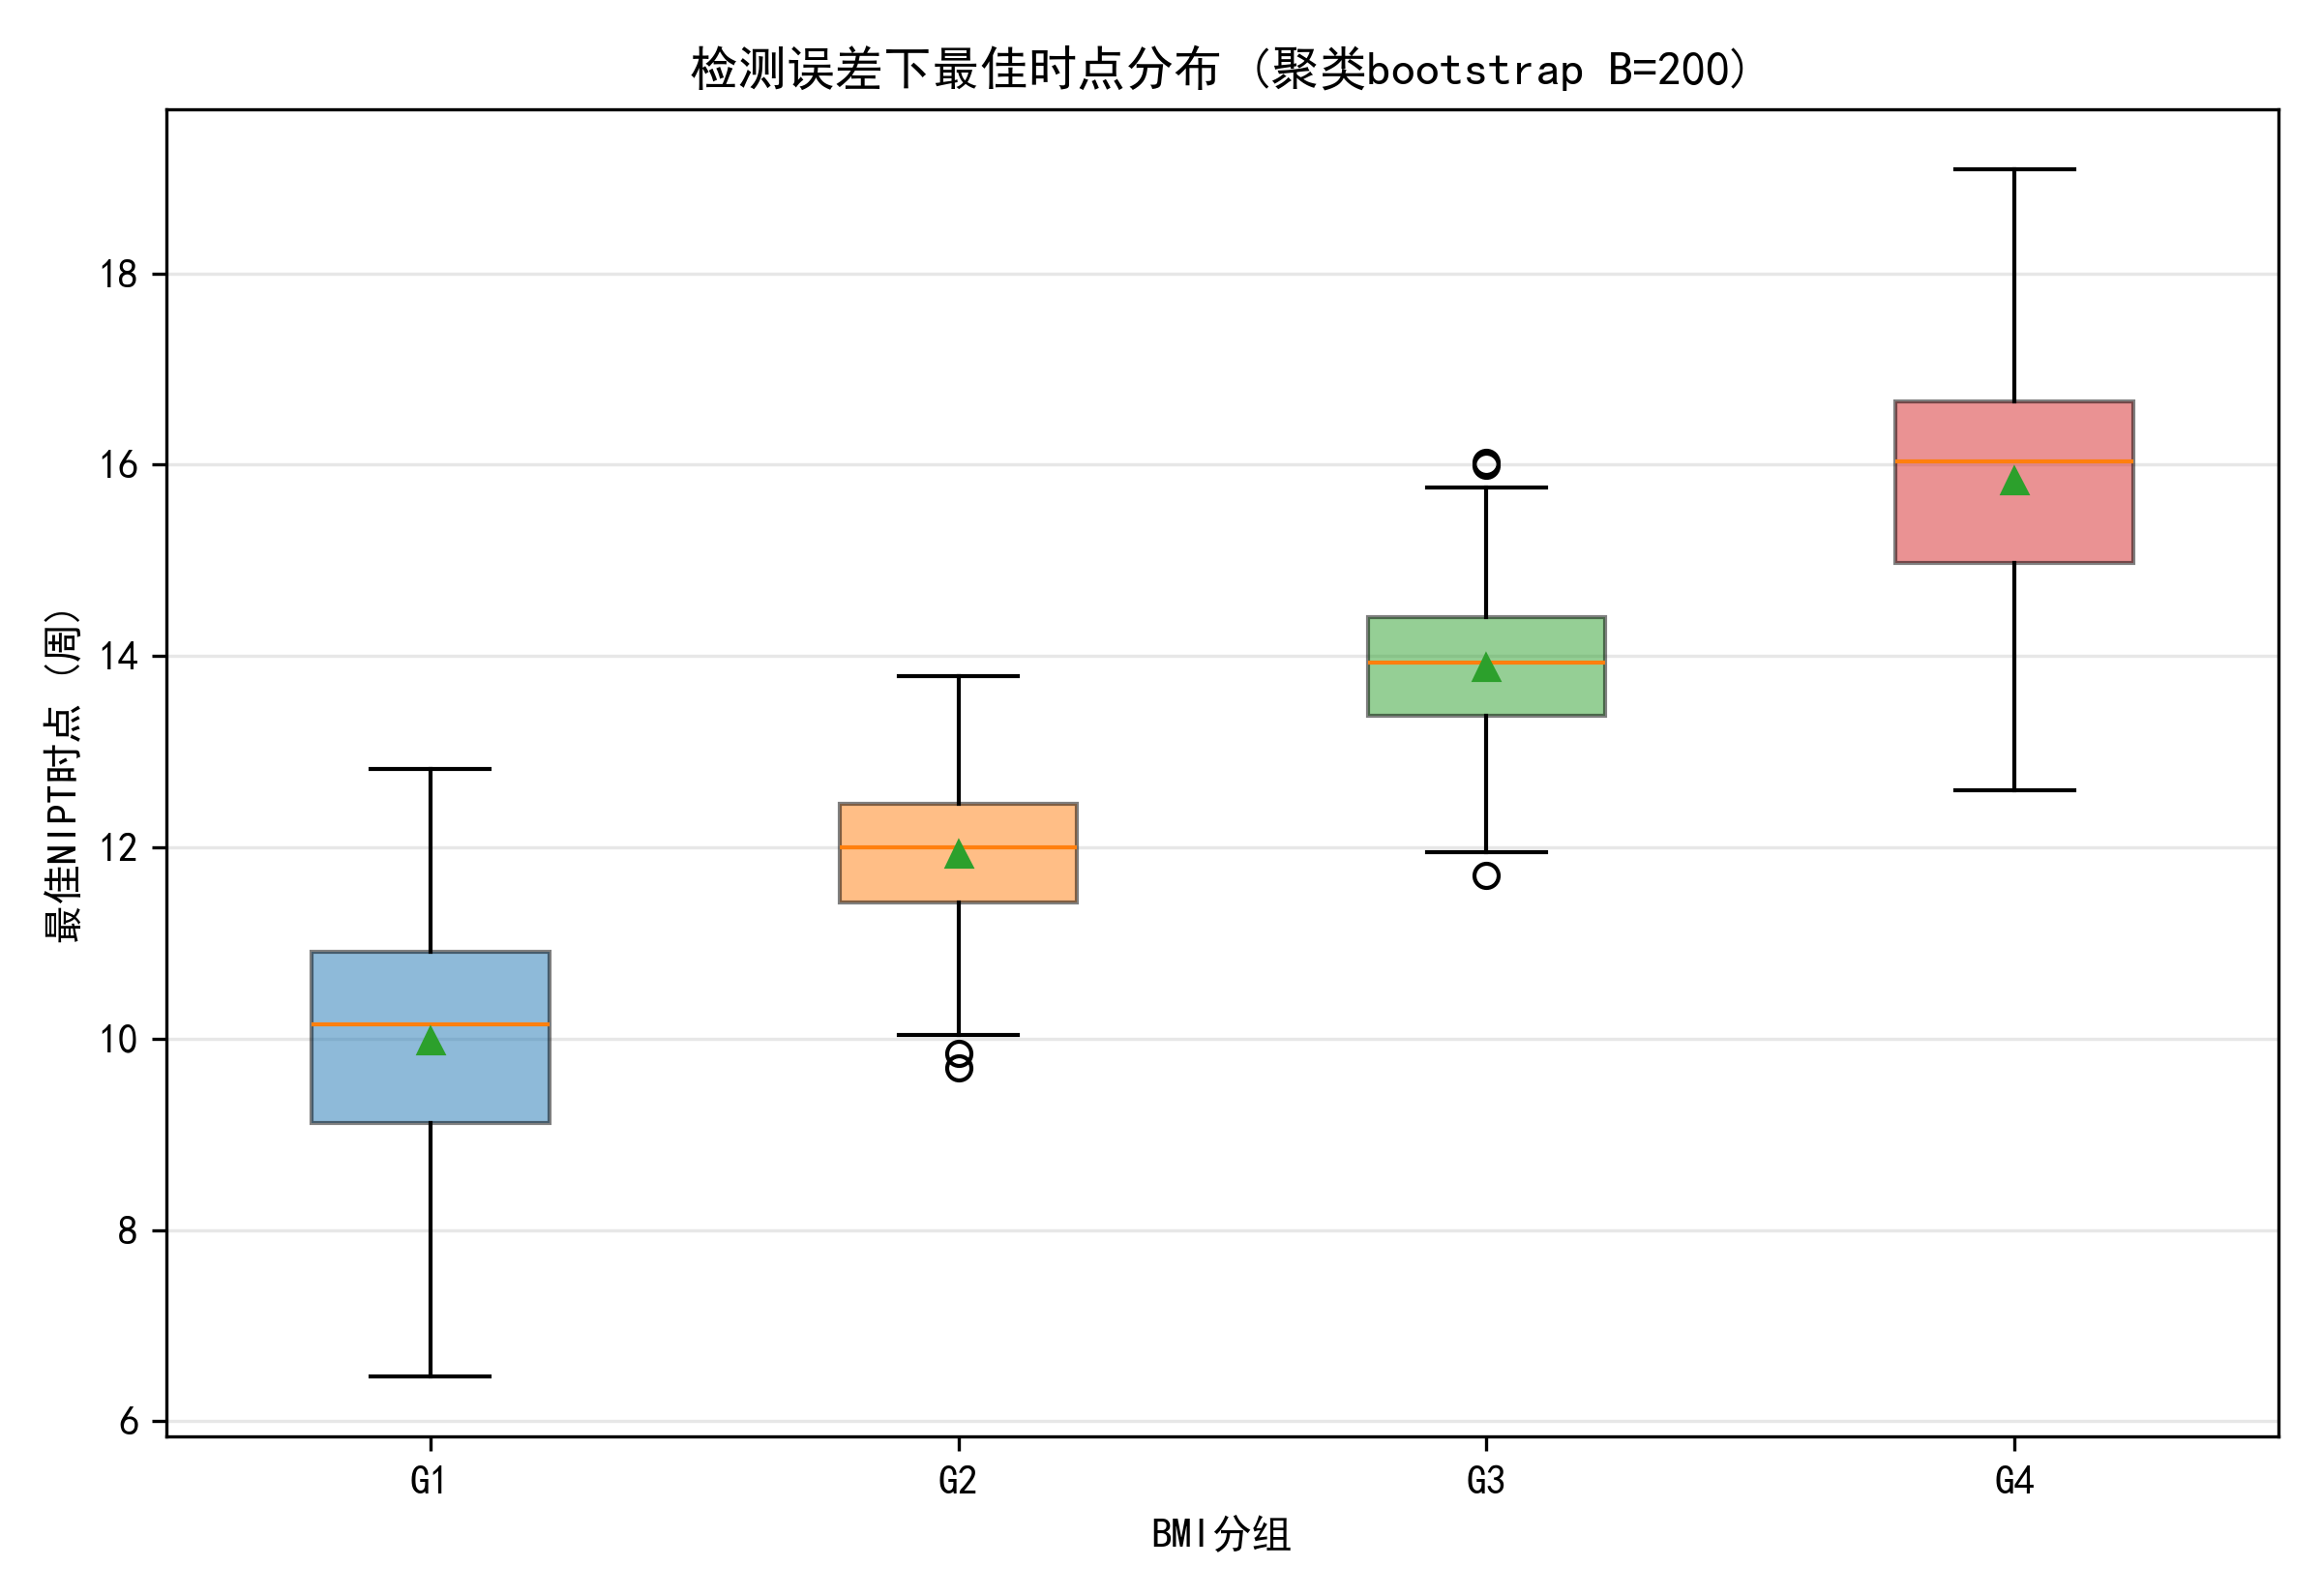
\includegraphics[width=0.8\textwidth]{output/figures/fig2-4_时点误差分布.png}
\caption{检测误差下各组最佳时点的分布（聚类bootstrap B=200）}
\label{fig:p2boot}
\end{figure}

\section{问题三：多因素综合的时点选择}

\subsection{多因素变量选择}

在问题二的基础上引入年龄、身高、体重等多因素。由于体重与BMI高度相关（$r=0.835$），二者不宜同时进入模型。以AIC准则进行变量选择，结果见表\ref{tab:aic}。模型M3（加入年龄与身高）AIC最小（$706.9$），而再加入体重的M4 AIC反而上升（$707.5$），证实体重与BMI共线。故最优模型为
\begin{equation}
\ln Y_{ij} = \beta_0 + \beta_1 t_c + \beta_2 \mathrm{BMI}_c + \beta_3 \mathrm{age}_c + \beta_4 \mathrm{height}_c + u_i + \varepsilon_{ij}.
\end{equation}

\begin{table}[H]
\centering
\caption{多因素模型变量选择（AIC/BIC）}
\label{tab:aic}
\begin{tabular}{llrr}
\toprule
模型 & 变量 & AIC & BIC \\
\midrule
M1 & week+BMI & 710.0 & 734.9 \\
M2 & +age & 709.0 & 738.9 \\
M3 & +age+height & \textbf{706.9} & 741.8 \\
M4 & +age+height+weight & 707.5 & 747.4 \\
\bottomrule
\end{tabular}
\end{table}

模型M3的系数估计见表\ref{tab:m3coef}。身高系数显著（$p=0.043$），年龄系数边缘显著（$p=0.118$），二者均为负，即高个子、高龄孕妇的胎儿DNA浓度略低。BMI仍为主导因素。

\begin{table}[H]
\centering
\caption{多因素模型系数（REML估计）}
\label{tab:m3coef}
\begin{tabular}{lrrr}
\toprule
变量 & 系数 & 标准误 & $p$值 \\
\midrule
截距 & $-2.652$ & 0.026 & $<0.001$ \\
孕周 & 0.0435 & 0.002 & $<0.001$ \\
BMI & $-0.0196$ & 0.007 & 0.008 \\
年龄 & $-0.0111$ & 0.007 & 0.118 \\
身高 & $-0.0102$ & 0.005 & 0.043 \\
\bottomrule
\end{tabular}
\end{table}

\subsection{达标比例与最佳时点}

以各组的中位BMI、年龄、身高作为代表孕妇，计算达标比例与最佳时点，结果见表\ref{tab:p3}。与问题二（仅BMI）相比，多因素修正幅度在$-0.54\sim+0.50$周之间，说明BMI仍是决定达标时点的主导因素，年龄与身高只起微调作用。

\begin{table}[H]
\centering
\caption{问题二与问题三最佳时点对比（单位：周）}
\label{tab:p3}
\begin{tabular}{lrrrr}
\toprule
分组 & BMI中位 & 仅BMI（问题二） & 多因素（问题三） & 差异 \\
\midrule
G1 & 27.6 & 10.82 & 10.59 & $-0.23$ \\
G2 & 30.4 & 12.11 & 11.57 & $-0.54$ \\
G3 & 33.5 & 13.59 & 13.23 & $-0.35$ \\
G4 & 37.3 & 15.39 & 15.89 & $+0.50$ \\
\bottomrule
\end{tabular}
\end{table}

图\ref{fig:p3curve}展示了多因素模型下各组的达标比例曲线，图\ref{fig:p3cmp}直观对比了问题二与问题三的最佳时点，可见多因素修正仅在$\pm0.5$周以内，两组结果高度一致，进一步印证BMI的主导作用；年龄与身高对最佳时点的影响见图\ref{fig:p3sens}。

\begin{figure}[H]
\centering
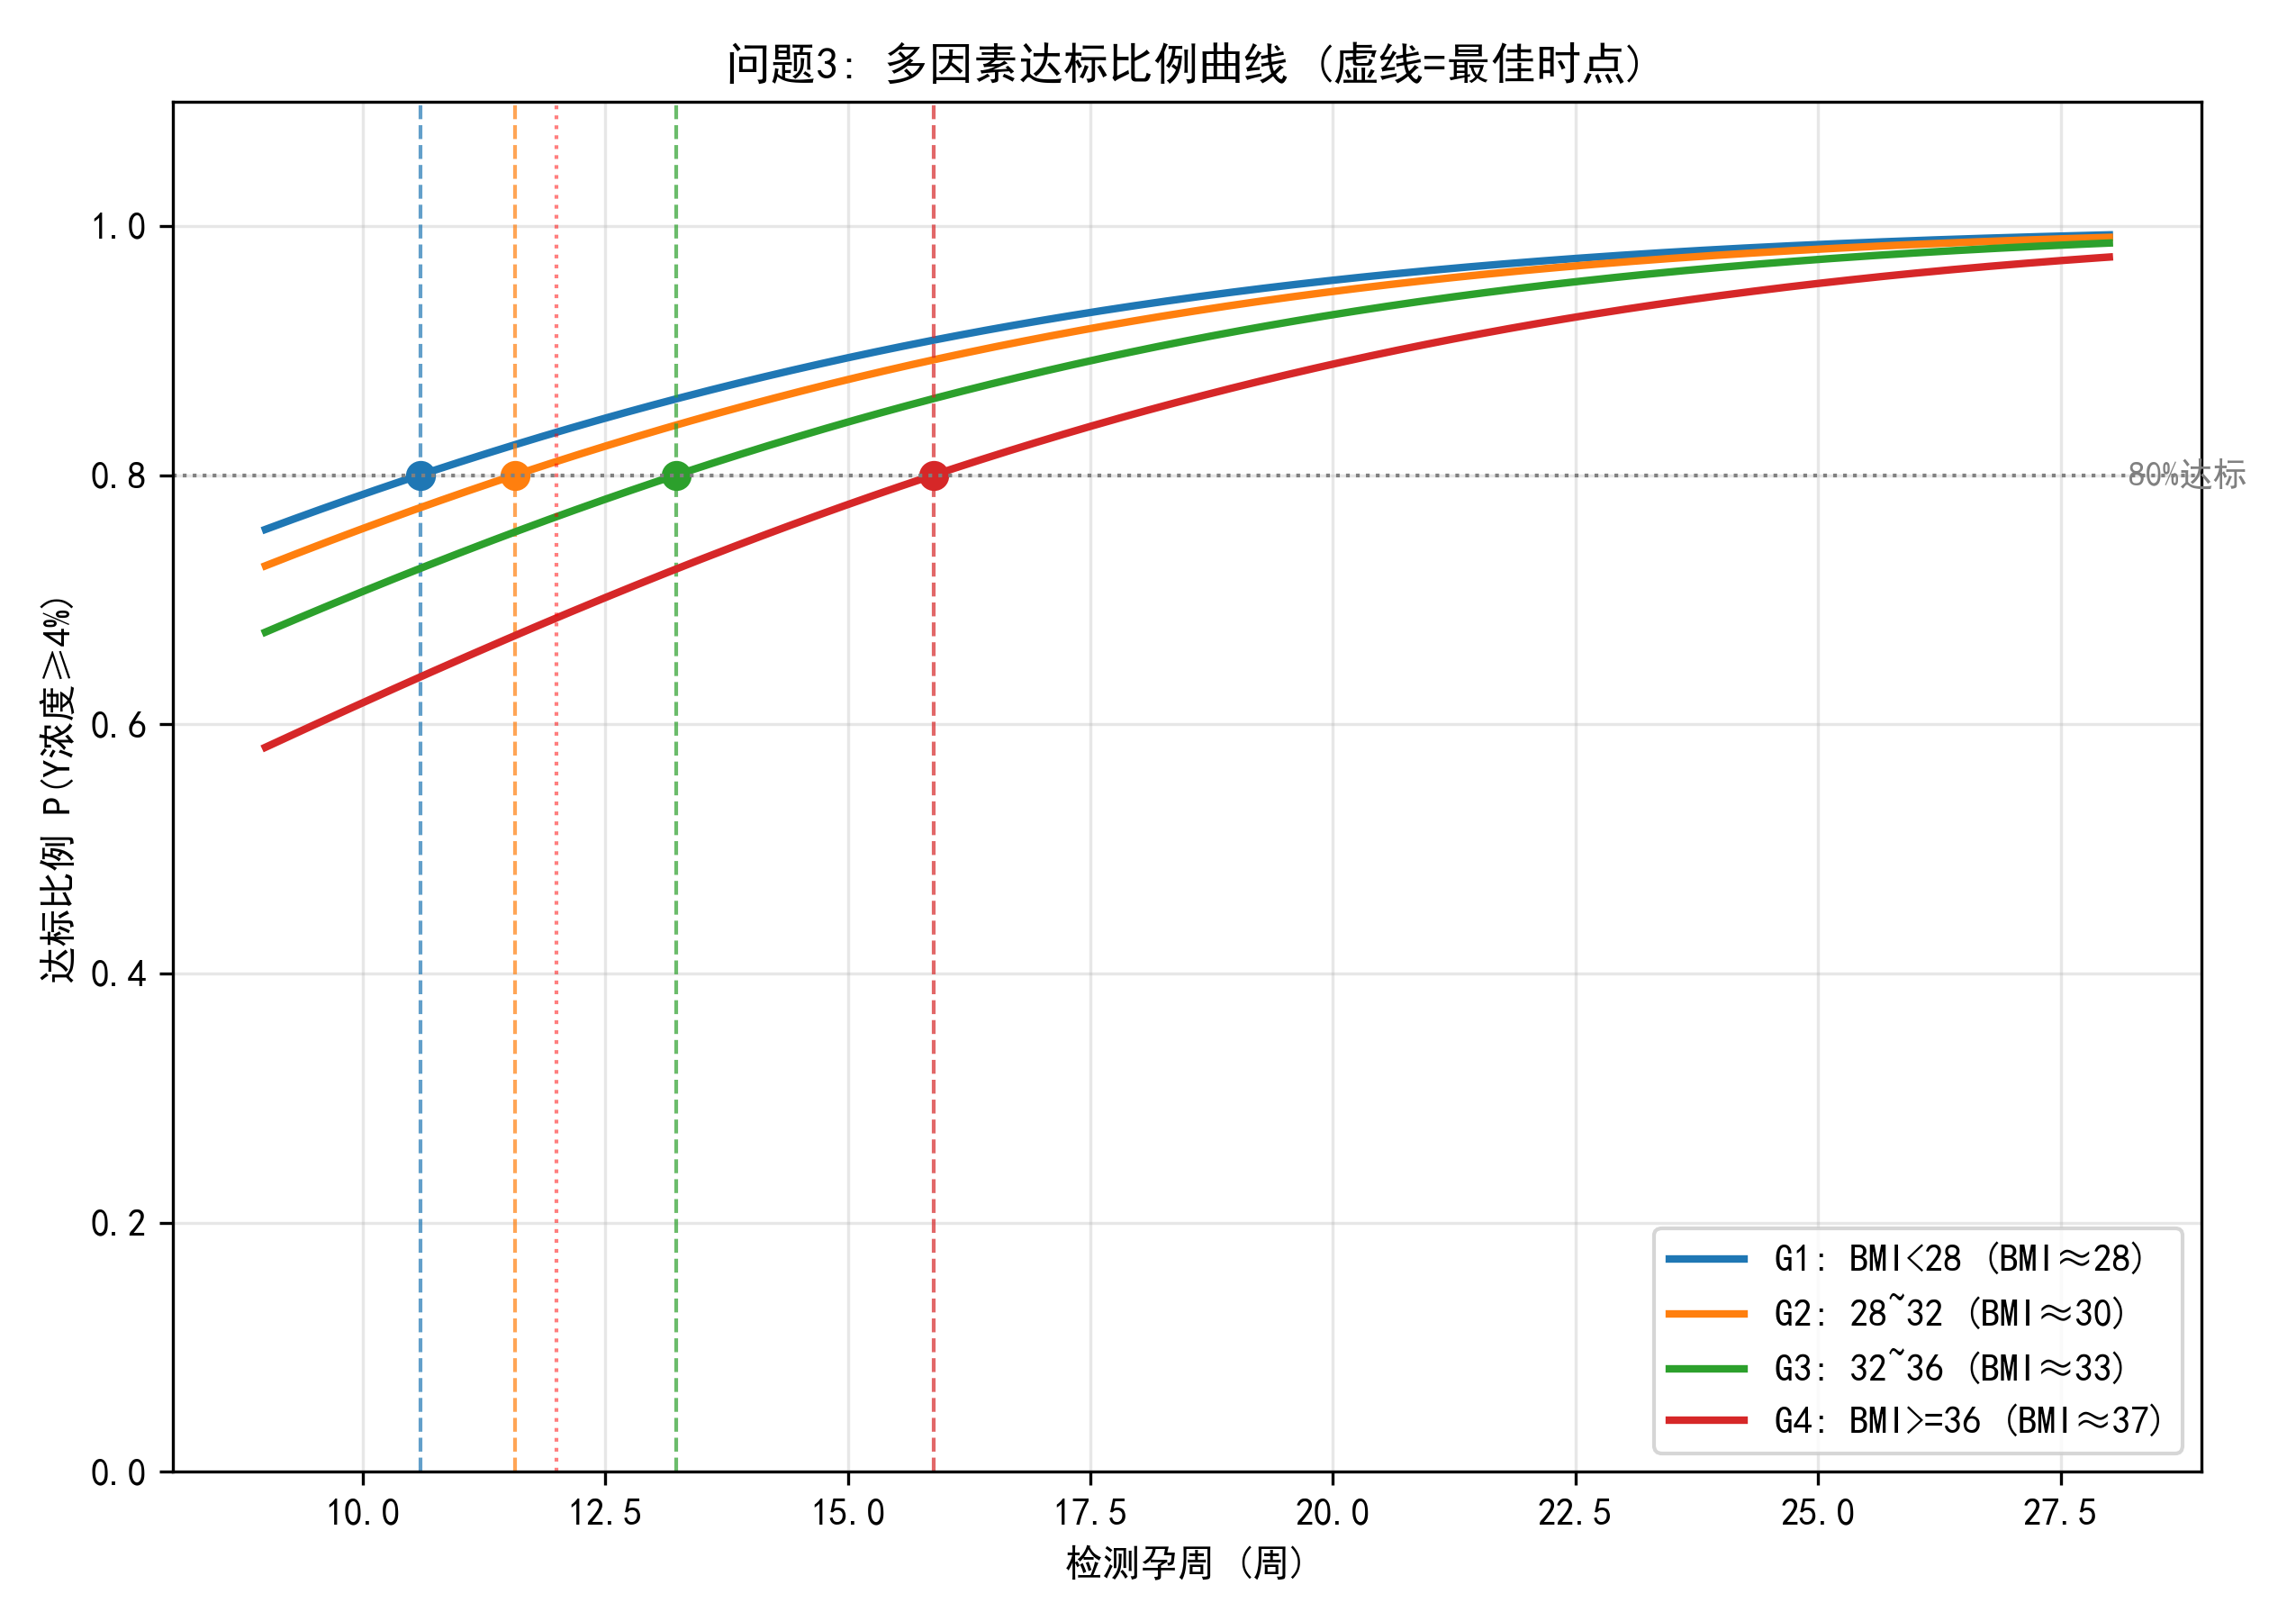
\includegraphics[width=0.85\textwidth]{output/figures/fig3-1_多因素达标比例.png}
\caption{多因素模型下各BMI组的达标比例曲线（虚线为最佳时点）}
\label{fig:p3curve}
\end{figure}

\begin{figure}[H]
\centering
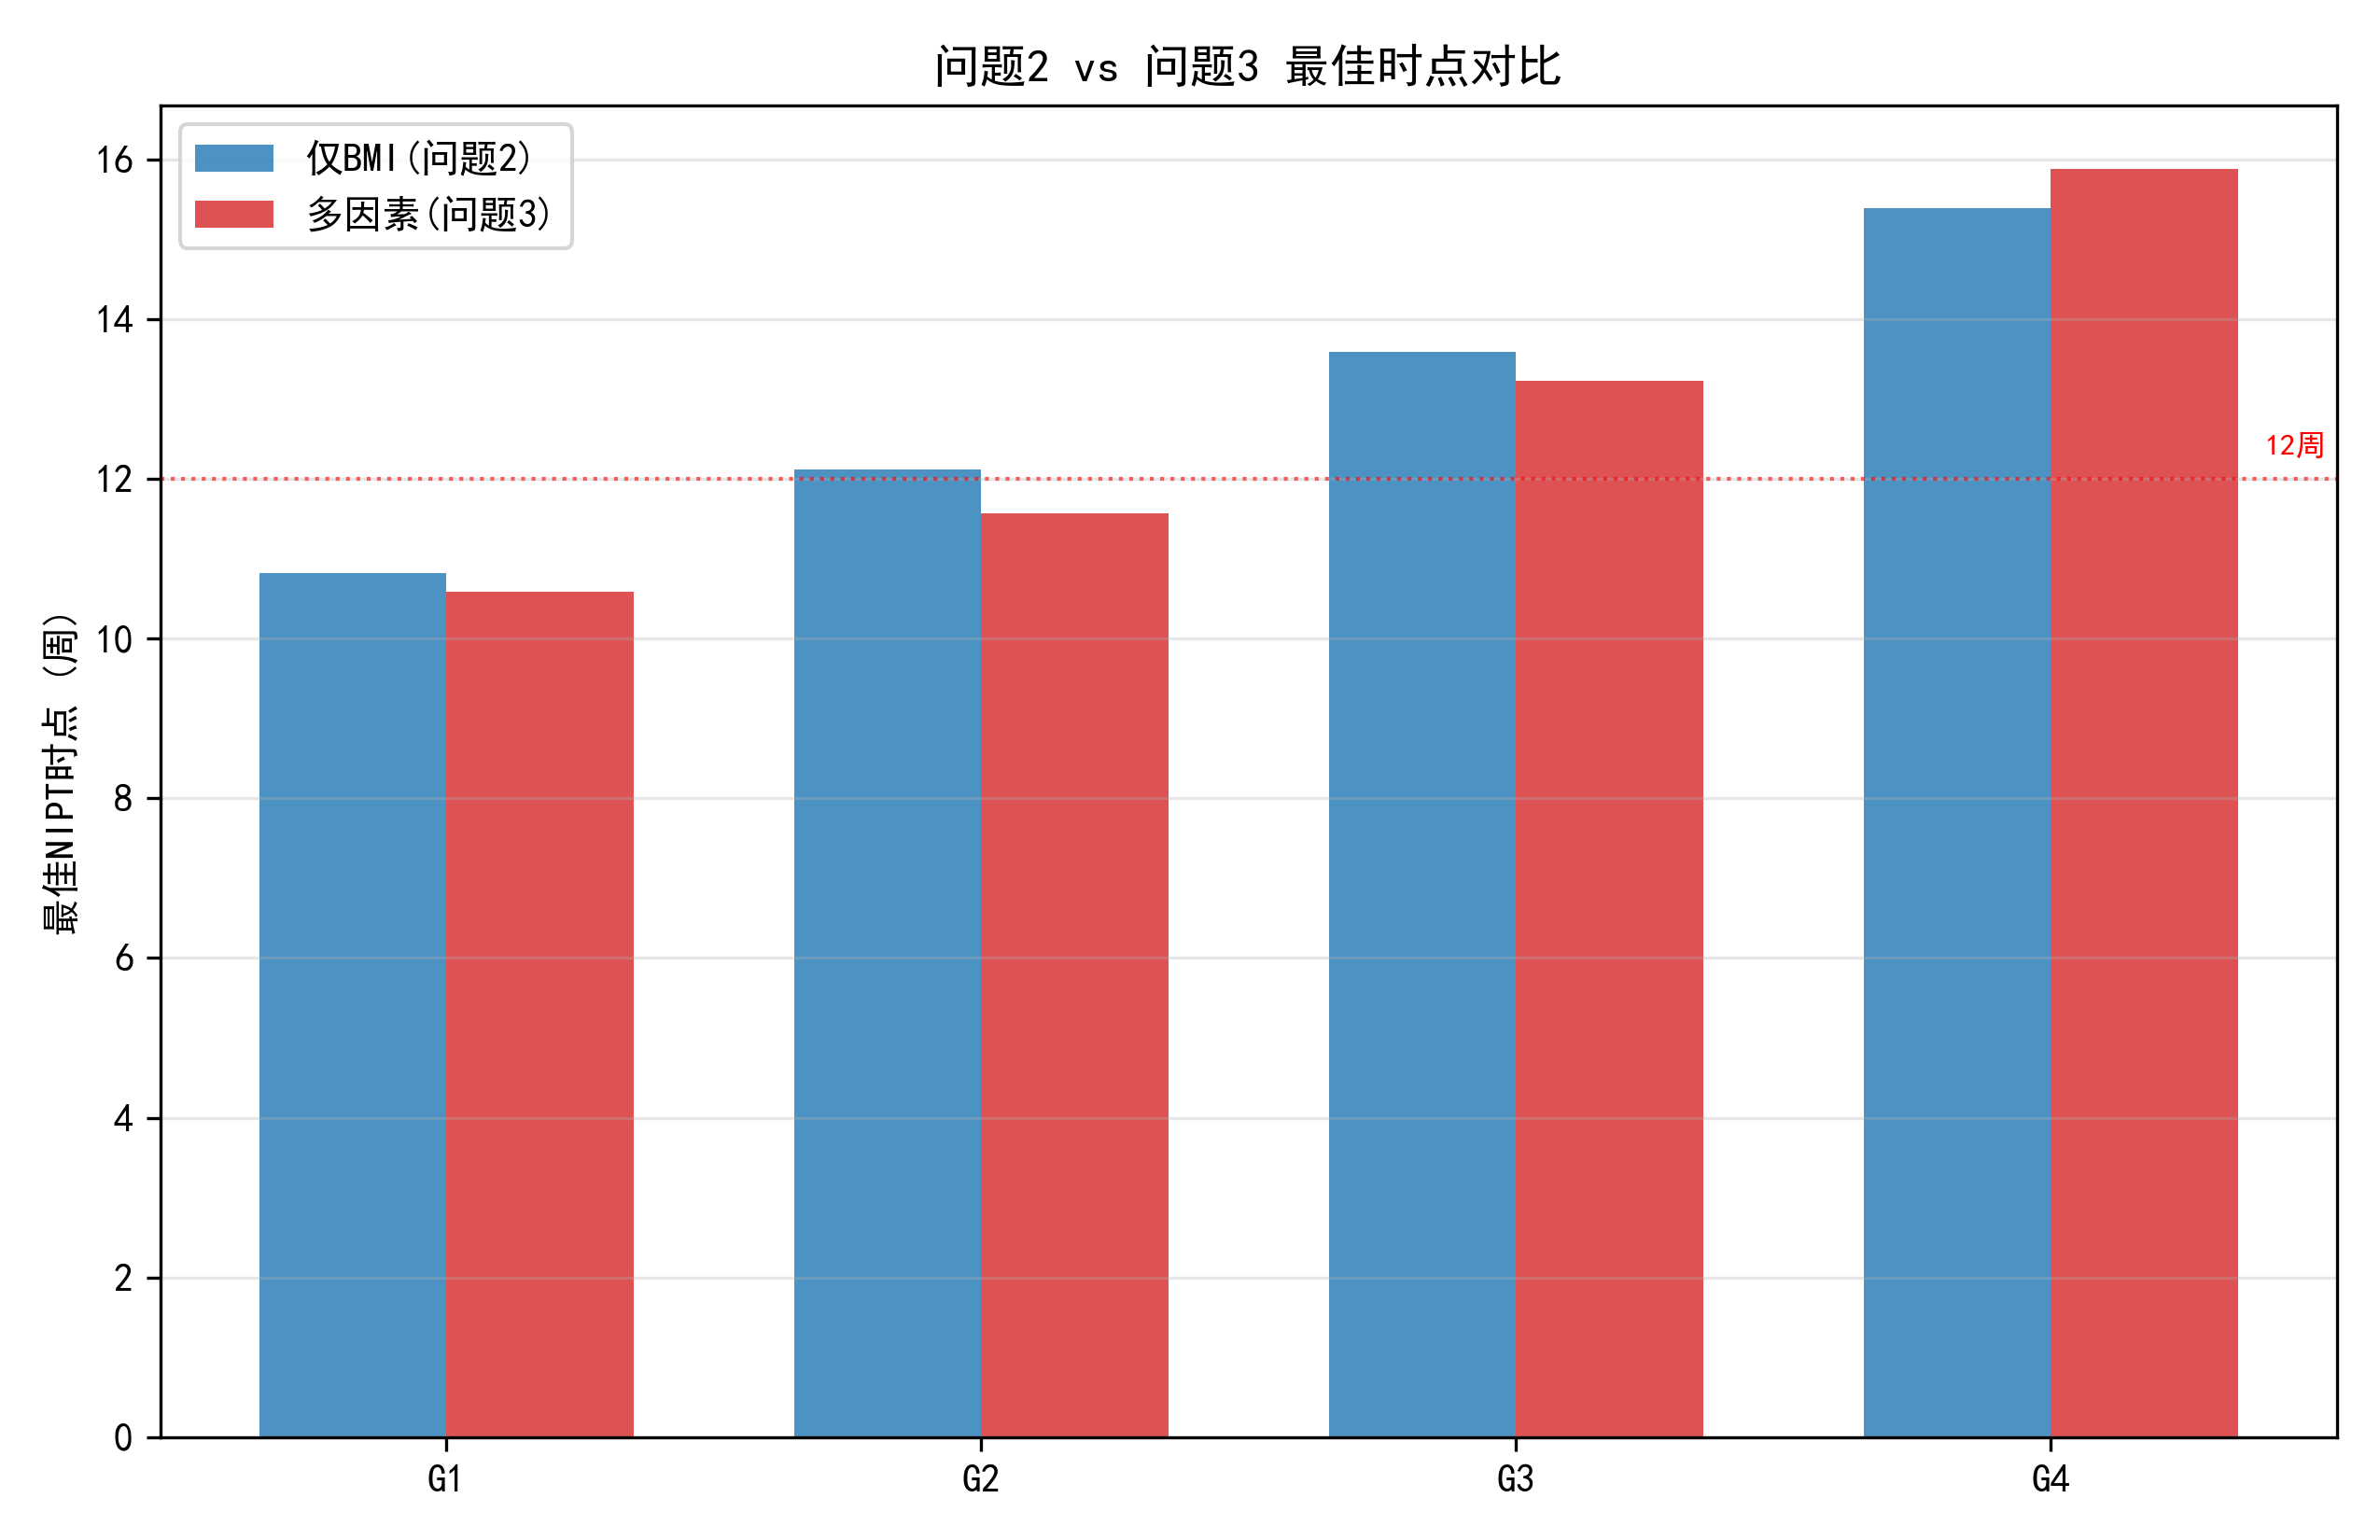
\includegraphics[width=0.8\textwidth]{output/figures/fig3-3_问题2vs3对比.png}
\caption{问题二（仅BMI）与问题三（多因素）最佳时点对比}
\label{fig:p3cmp}
\end{figure}

\begin{figure}[H]
\centering
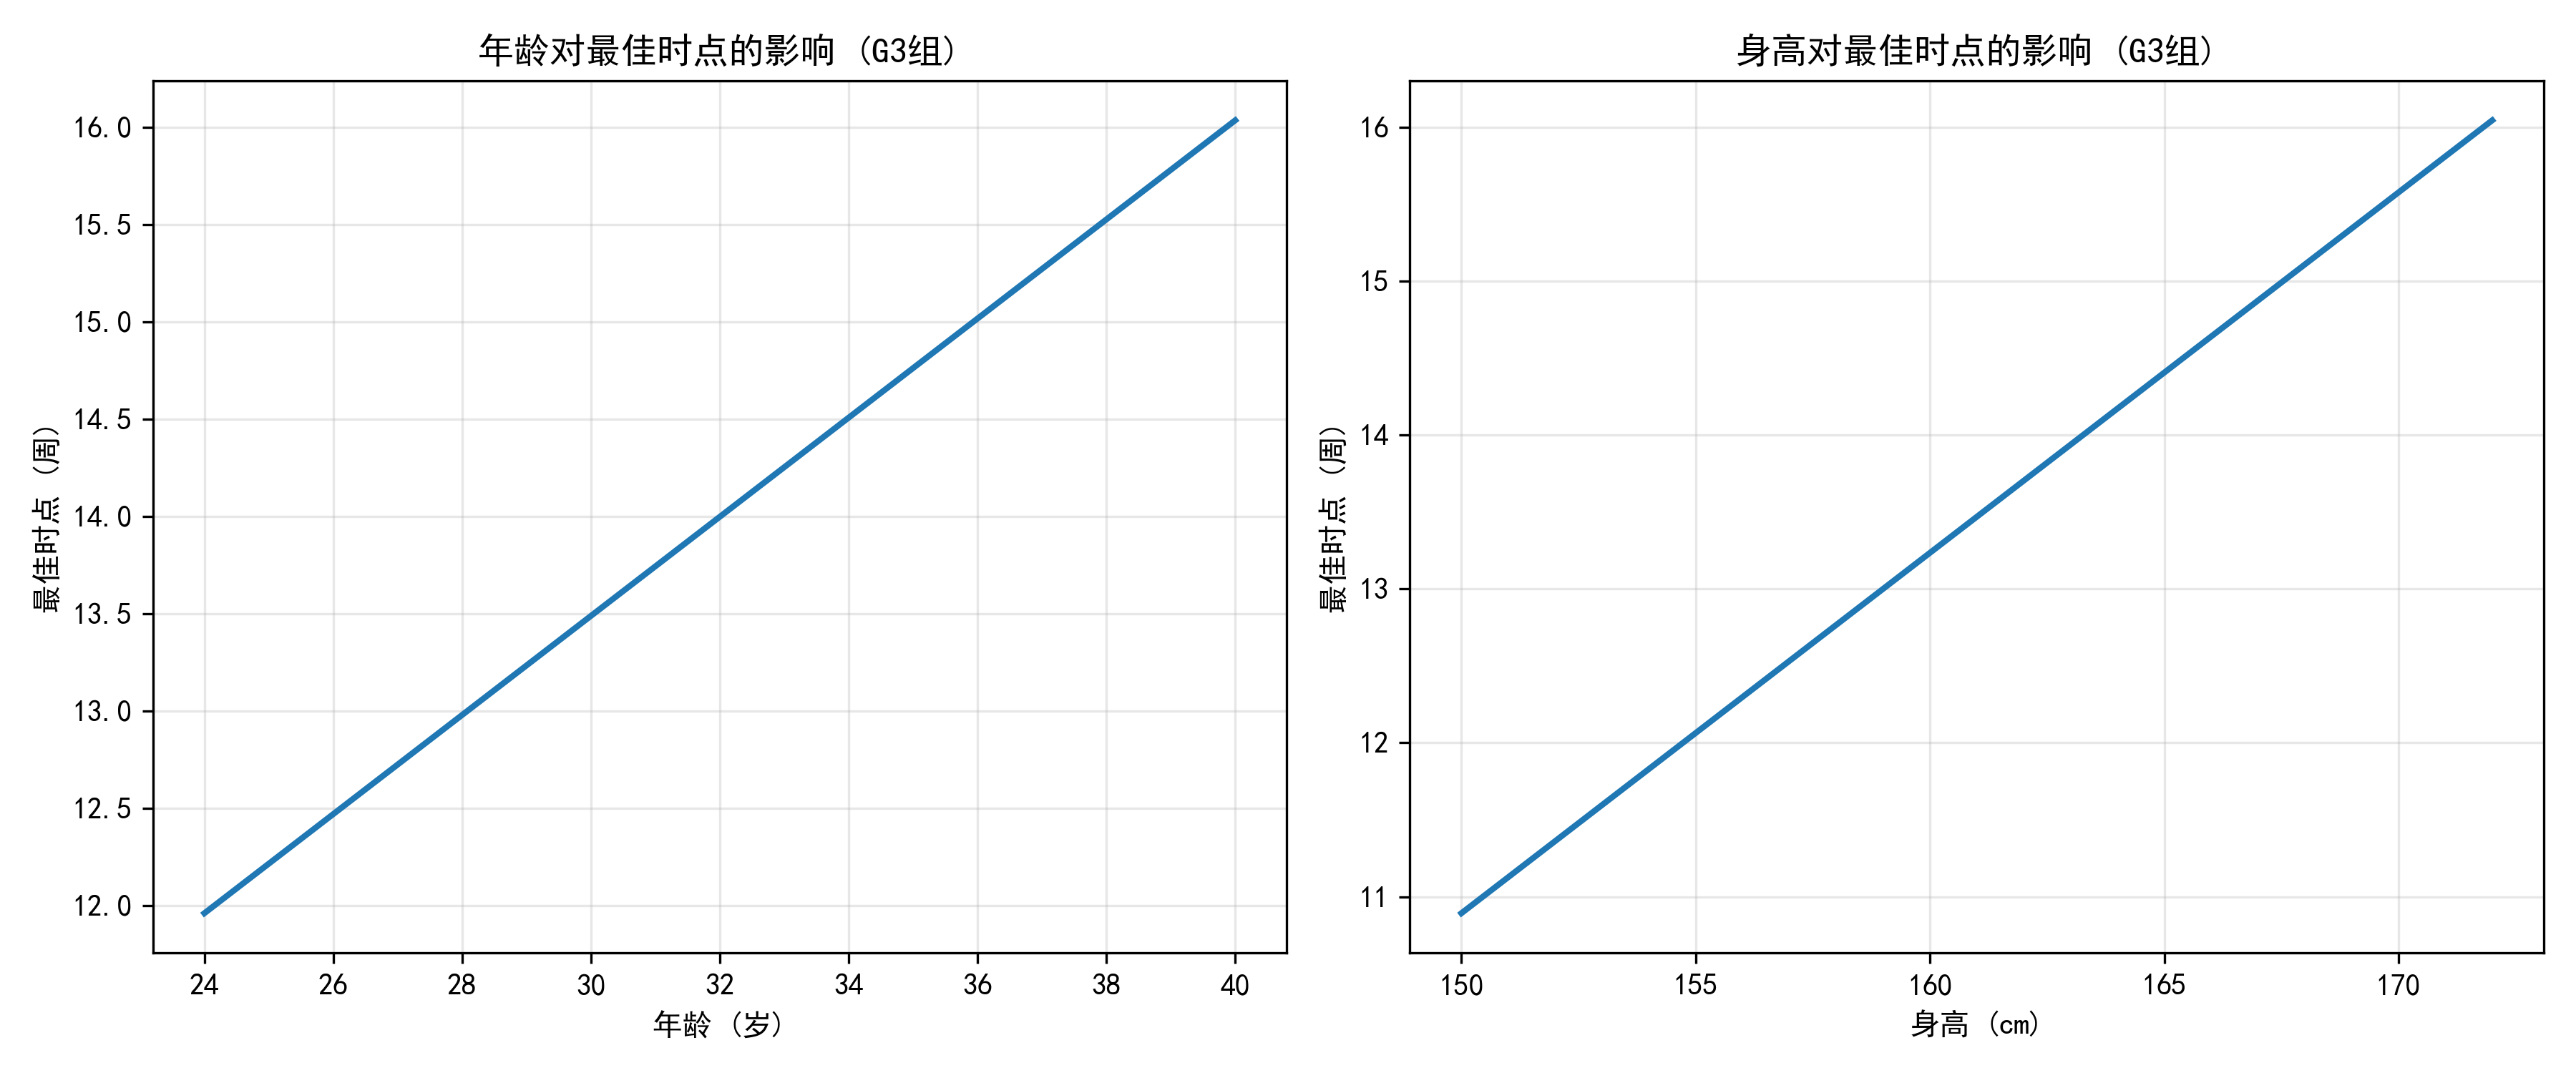
\includegraphics[width=0.95\textwidth]{output/figures/fig3-2_年龄身高敏感性.png}
\caption{年龄与身高对最佳时点的影响（G3组，敏感性分析）}
\label{fig:p3sens}
\end{figure}

\subsection{测量误差敏感性}

固定G3组（BMI中位$33.5$），将测量误差$\sigma_e$在$0.5\sim1.5$倍之间缩放，观察最佳时点的变化，结果见表\ref{tab:sens}。测量误差越大，为保证达标比例，最佳时点越向后推迟；$\sigma_e$从$0.124$增至$0.372$时，时点从$12.23$周推迟到$14.70$周，推迟约$2.5$周。这提示控制测序质量、降低测量误差可显著提前检测时点，检测误差对时点分布的影响见图\ref{fig:p3boot}。

\begin{table}[H]
\centering
\caption{测量误差$\sigma_e$对最佳时点的影响（G3组）}
\label{tab:sens}
\begin{tabular}{lrrrrr}
\toprule
$\sigma_e$倍数 & 0.50 & 0.75 & 1.00 & 1.25 & 1.50 \\
\midrule
$\sigma_e$ & 0.124 & 0.186 & 0.248 & 0.310 & 0.372 \\
最佳时点（周） & 12.23 & 12.66 & 13.23 & 13.92 & 14.70 \\
\bottomrule
\end{tabular}
\end{table}

\begin{figure}[H]
\centering
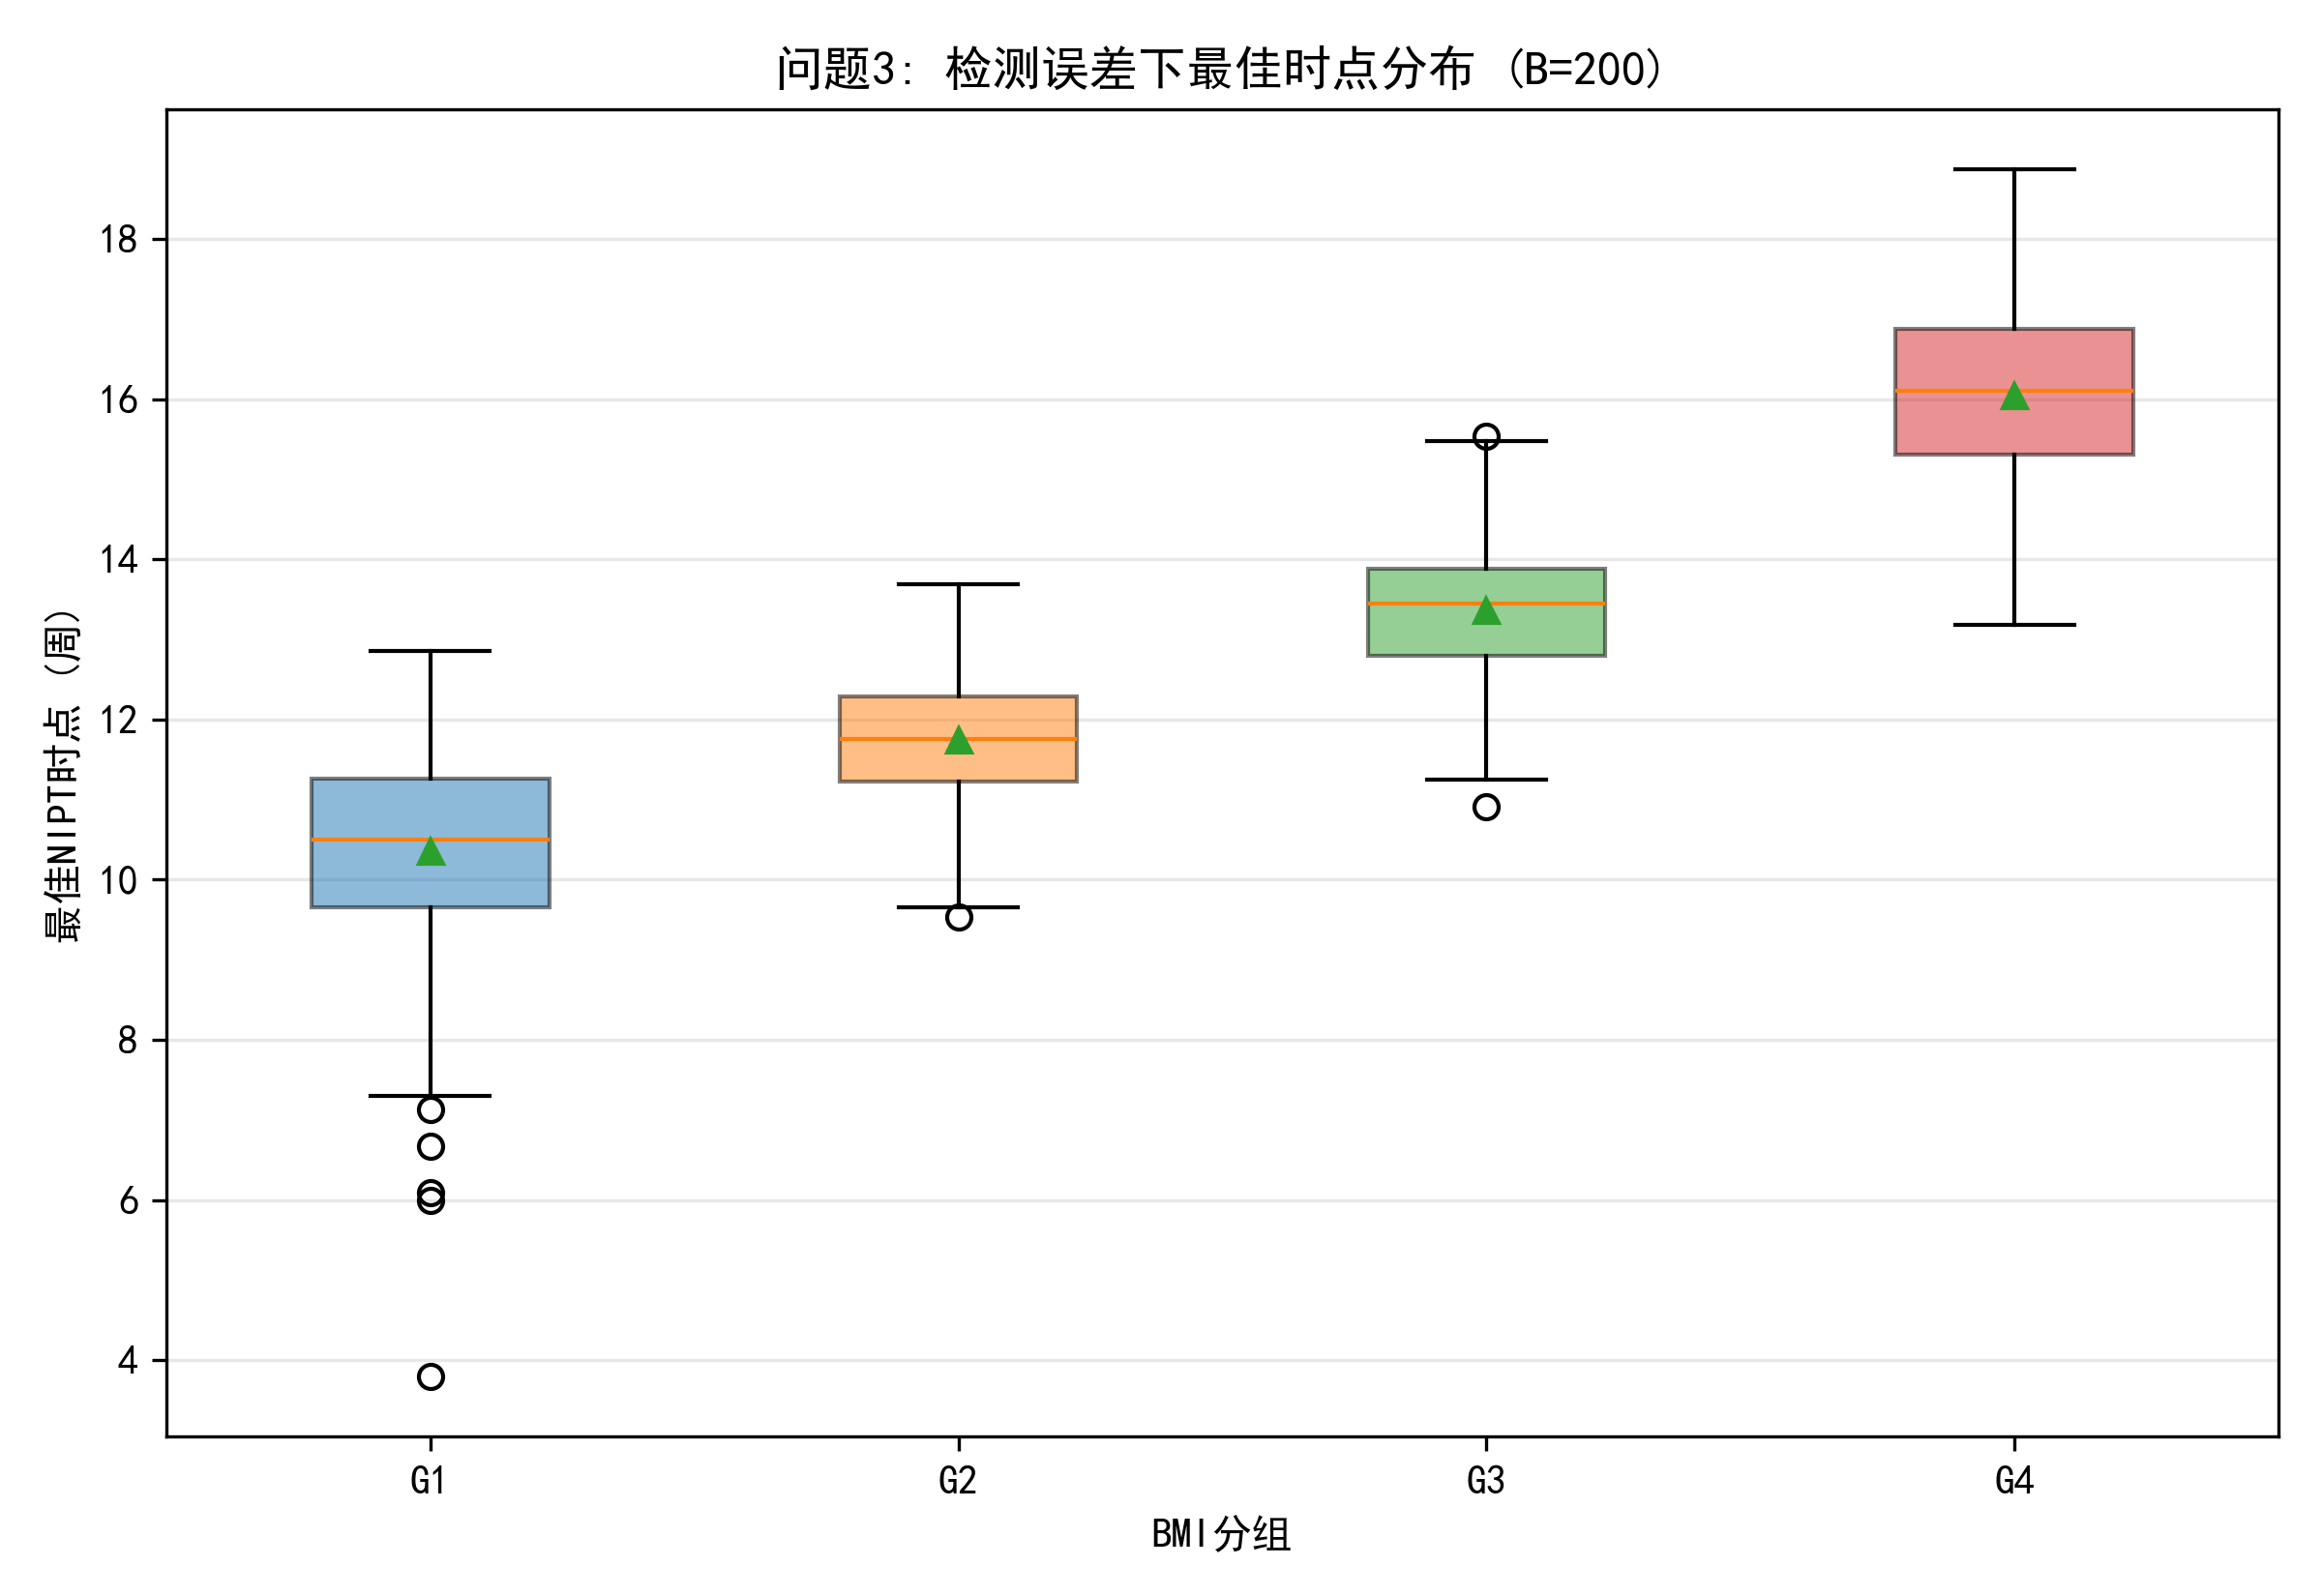
\includegraphics[width=0.8\textwidth]{output/figures/fig3-4_时点误差分布.png}
\caption{多因素模型下检测误差对最佳时点的影响（聚类bootstrap B=200）}
\label{fig:p3boot}
\end{figure}

\section{问题四：女胎异常判定}

\subsection{数据与特征}

女胎检测数据共605条（147位孕妇），其中正常538例、异常67例（非整倍体占$11.1\%$），类别不平衡。异常类型包括T18（33例）、T13T18（11例）、T13（10例）、T21（9例）等。特征包括13/18/21号染色体Z值、X染色体Z值与浓度、各染色体GC含量、读段数及比对/重复/过滤比例、BMI、年龄、身高、体重、孕周共26维。

关键观察：异常样本的Z值并未显著偏离正常。如表\ref{tab:z}所示，T18样本的18号Z值均值仅$1.03$，远低于$3$的阈值；异常样本中$|Z|>3$的比例仅为$0\sim4.5\%$。这说明传统的$|Z|>3$阈值法难以复现AB列的判定，异常标签是由多因素共同作用的结果。图\ref{fig:zdist}直观对比了正常与异常样本的Z值分布。

\begin{table}[H]
\centering
\caption{各异常类型的对应染色体Z值均值}
\label{tab:z}
\begin{tabular}{lrrrr}
\toprule
异常类型 & 样本量 & Z13 & Z18 & Z21 \\
\midrule
T13 & 10 & $-0.20$ & 0.28 & 0.39 \\
T18 & 33 & 0.49 & 1.03 & $-0.16$ \\
T21 & 9 & 0.02 & 0.44 & 0.27 \\
T13T18 & 11 & 0.52 & 0.73 & 0.65 \\
\bottomrule
\end{tabular}
\end{table}

\begin{figure}[H]
\centering
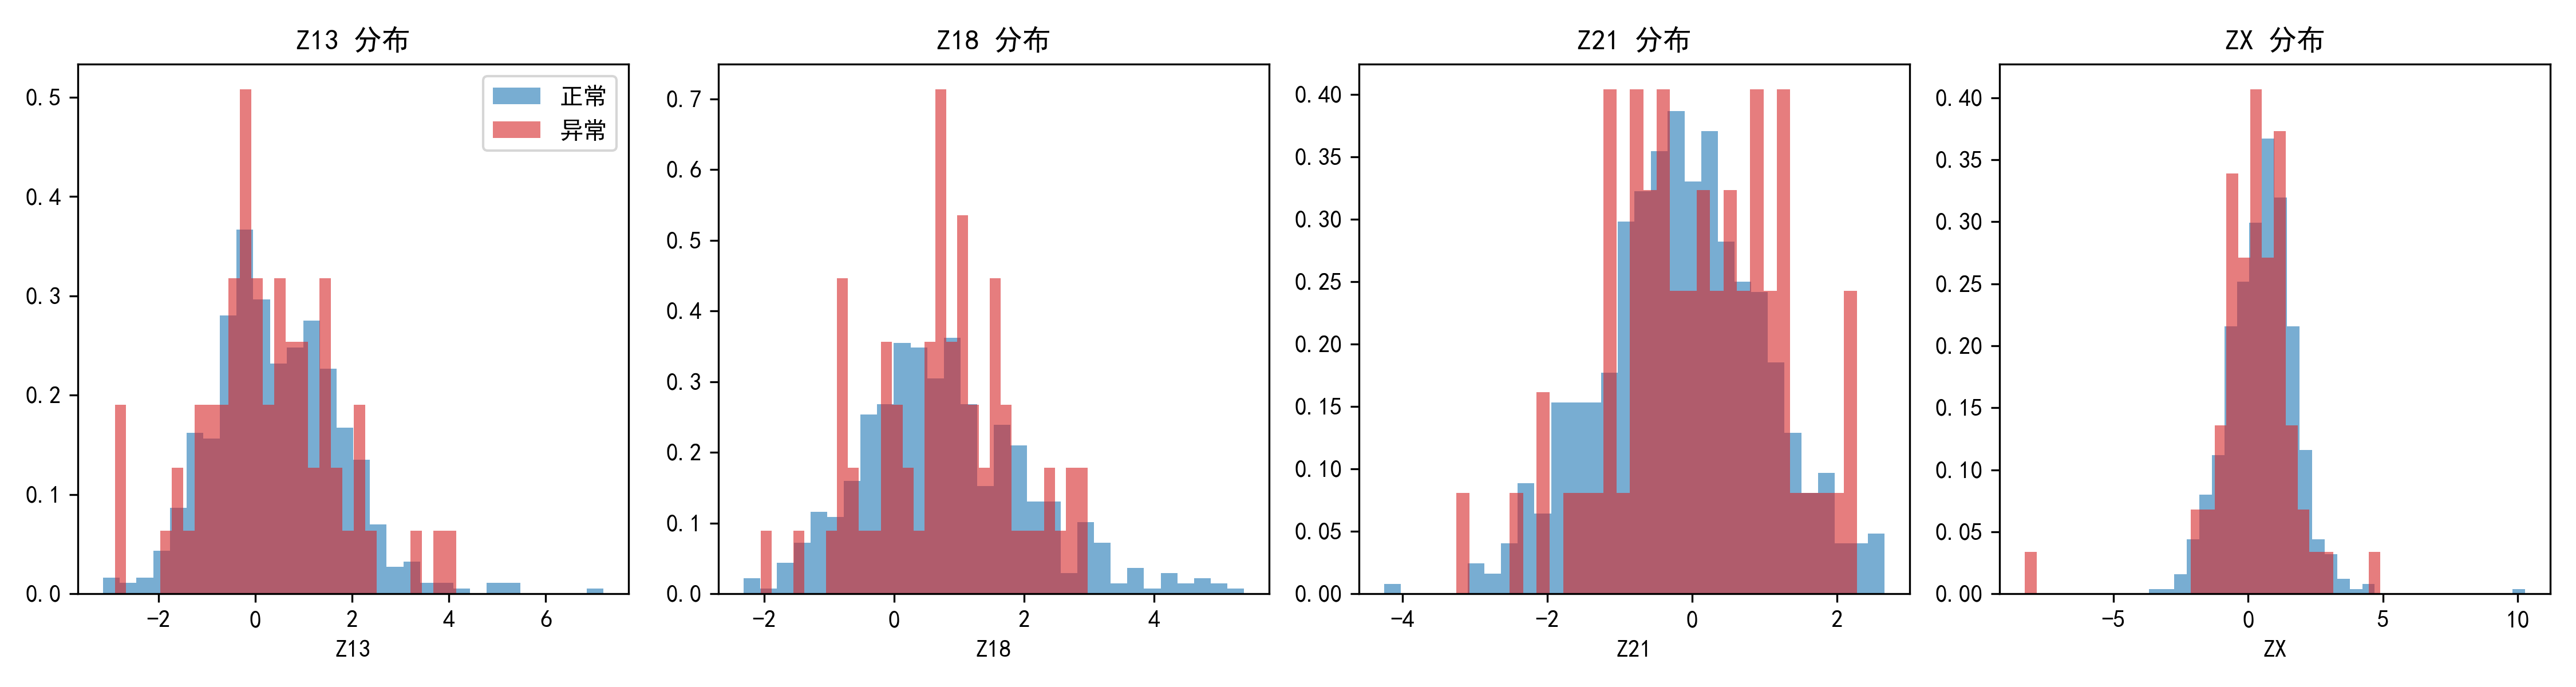
\includegraphics[width=0.95\textwidth]{output/figures/fig4-4_Z值分布对比.png}
\caption{正常与异常样本的Z值分布对比（异常样本Z值未显著偏离）}
\label{fig:zdist}
\end{figure}

\subsection{判定方法}

构建三类模型进行对比：传统Z值阈值法（$|Z|>3$判异常）作为基线，逻辑回归与随机森林、梯度提升作为综合多特征的机器学习方法。针对类别不平衡，逻辑回归采用平衡类权重，随机森林采用平衡类权重，并以分层5折交叉验证评估。特征工程包括Z值的绝对值、多染色体Z值联合、GC偏离正常中值的程度、X染色体浓度的绝对值等。

\subsection{结果与评估}

各模型性能见表\ref{tab:p4}与图\ref{fig:p4roc}。Z值阈值法敏感度仅$6.0\%$，几乎无法识别异常，说明单靠Z值阈值判定失效。逻辑回归AUC达$0.794$，敏感度$0.669$、特异度$0.812$；随机森林AUC同为$0.794$，特异度更高（$0.963$）但敏感度较低（$0.327$）。对于异常判定这一"漏诊代价高"的场景，逻辑回归在敏感度上更优，可作为推荐方法。

\begin{table}[H]
\centering
\caption{各模型5折交叉验证性能}
\label{tab:p4}
\begin{tabular}{lrrrrr}
\toprule
模型 & AUC & F1 & 敏感度 & 精确率 & 特异度 \\
\midrule
Z值阈值法 & --- & 0.071 & 0.060 & 0.089 & 0.924 \\
逻辑回归 & 0.794 & 0.416 & 0.669 & 0.304 & 0.812 \\
随机森林 & 0.794 & 0.394 & 0.327 & 0.543 & 0.963 \\
梯度提升 & 0.785 & 0.341 & 0.269 & 0.530 & 0.967 \\
\bottomrule
\end{tabular}
\end{table}

\begin{figure}[H]
\centering
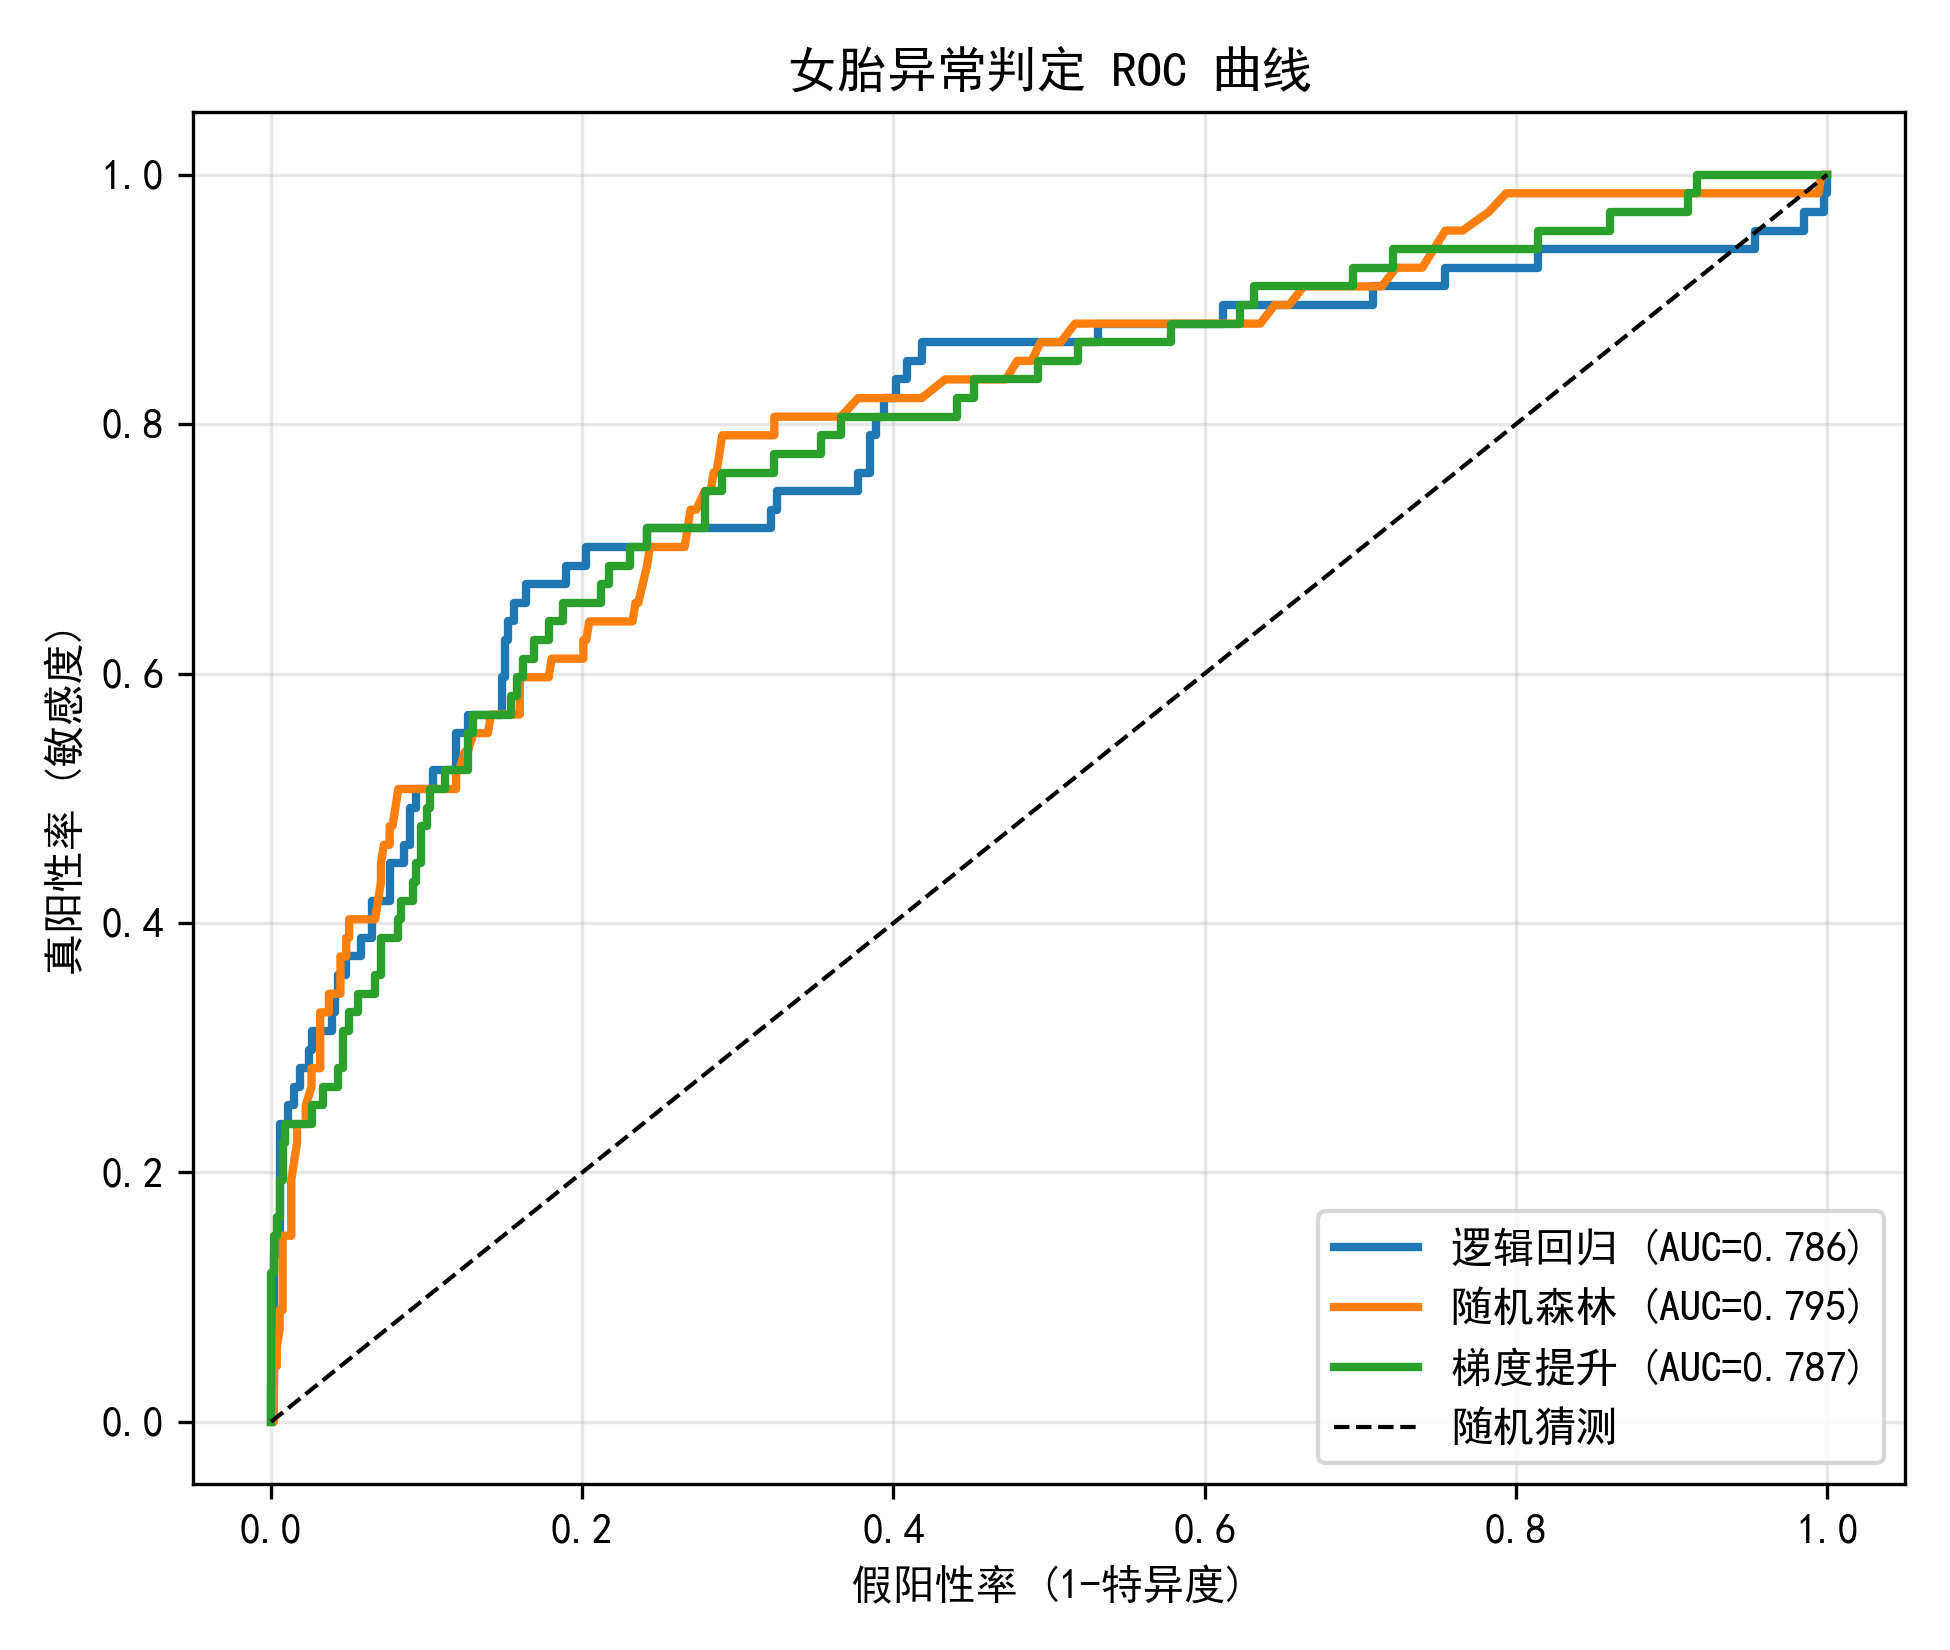
\includegraphics[width=0.8\textwidth]{output/figures/fig4-1_ROC曲线.png}
\caption{女胎异常判定的ROC曲线}
\label{fig:p4roc}
\end{figure}

由于类别不平衡（异常仅占$11.1\%$），精确率-召回率（PR）曲线比ROC更能反映判定质量。图\ref{fig:p4pr}显示逻辑回归的PR曲线整体优于随机森林与梯度提升，逻辑回归的平均精确率AP为$0.458$，随机森林与梯度提升分别为$0.405$与$0.446$。

\begin{figure}[H]
\centering
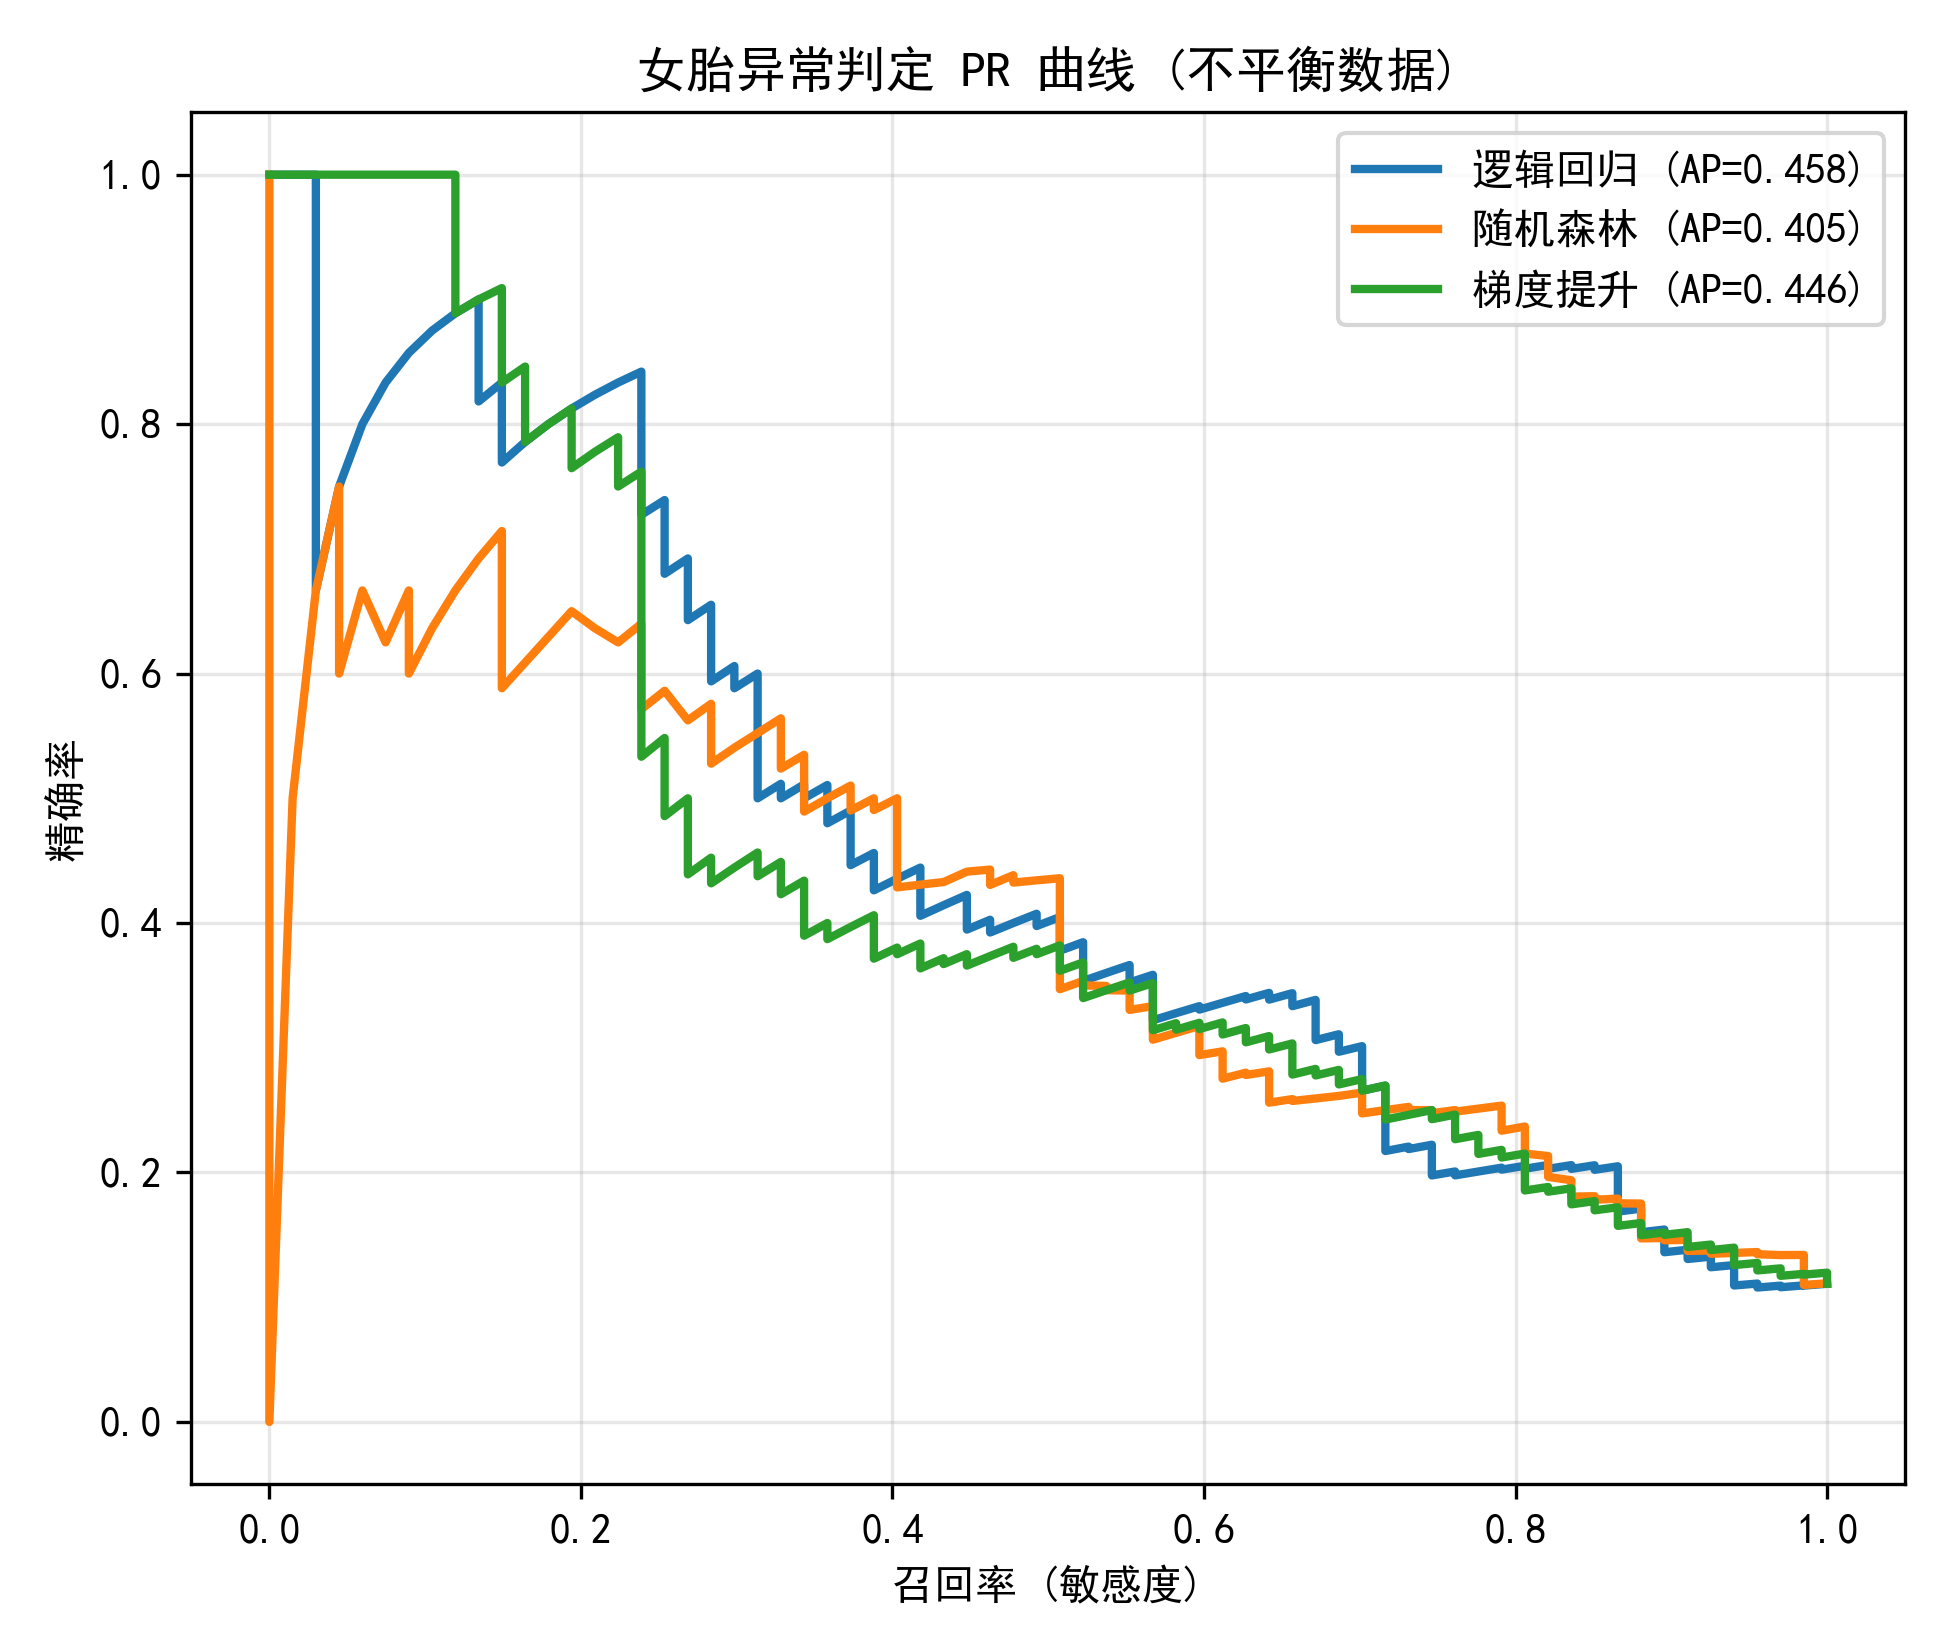
\includegraphics[width=0.78\textwidth]{output/figures/fig4-2_PR曲线.png}
\caption{女胎异常判定的精确率-召回率曲线（不平衡数据）}
\label{fig:p4pr}
\end{figure}

特征重要性（表\ref{tab:imp}与图\ref{fig:p4imp}）显示，X染色体浓度（$X_{\rm conc}$及其绝对值）是最重要的判别特征，其次为各染色体的GC含量与BMI。这与题目背景"女胎以X染色体浓度判断检测是否准确"完全一致，说明女胎异常判定首先依赖X染色体信息的可靠性，再结合GC含量等测序质量指标综合判断。

\begin{table}[H]
\centering
\caption{随机森林特征重要性（前6位）}
\label{tab:imp}
\begin{tabular}{lrr}
\toprule
特征 & 重要性 & 说明 \\
\midrule
$X_{\rm conc}$ & 0.138 & X染色体浓度 \\
$|X_{\rm conc}|$ & 0.096 & X浓度绝对偏离 \\
GC13 & 0.065 & 13号染色体GC含量 \\
GC21 & 0.052 & 21号染色体GC含量 \\
GC18 & 0.051 & 18号染色体GC含量 \\
BMI & 0.051 & 孕妇BMI \\
\bottomrule
\end{tabular}
\end{table}

\begin{figure}[H]
\centering
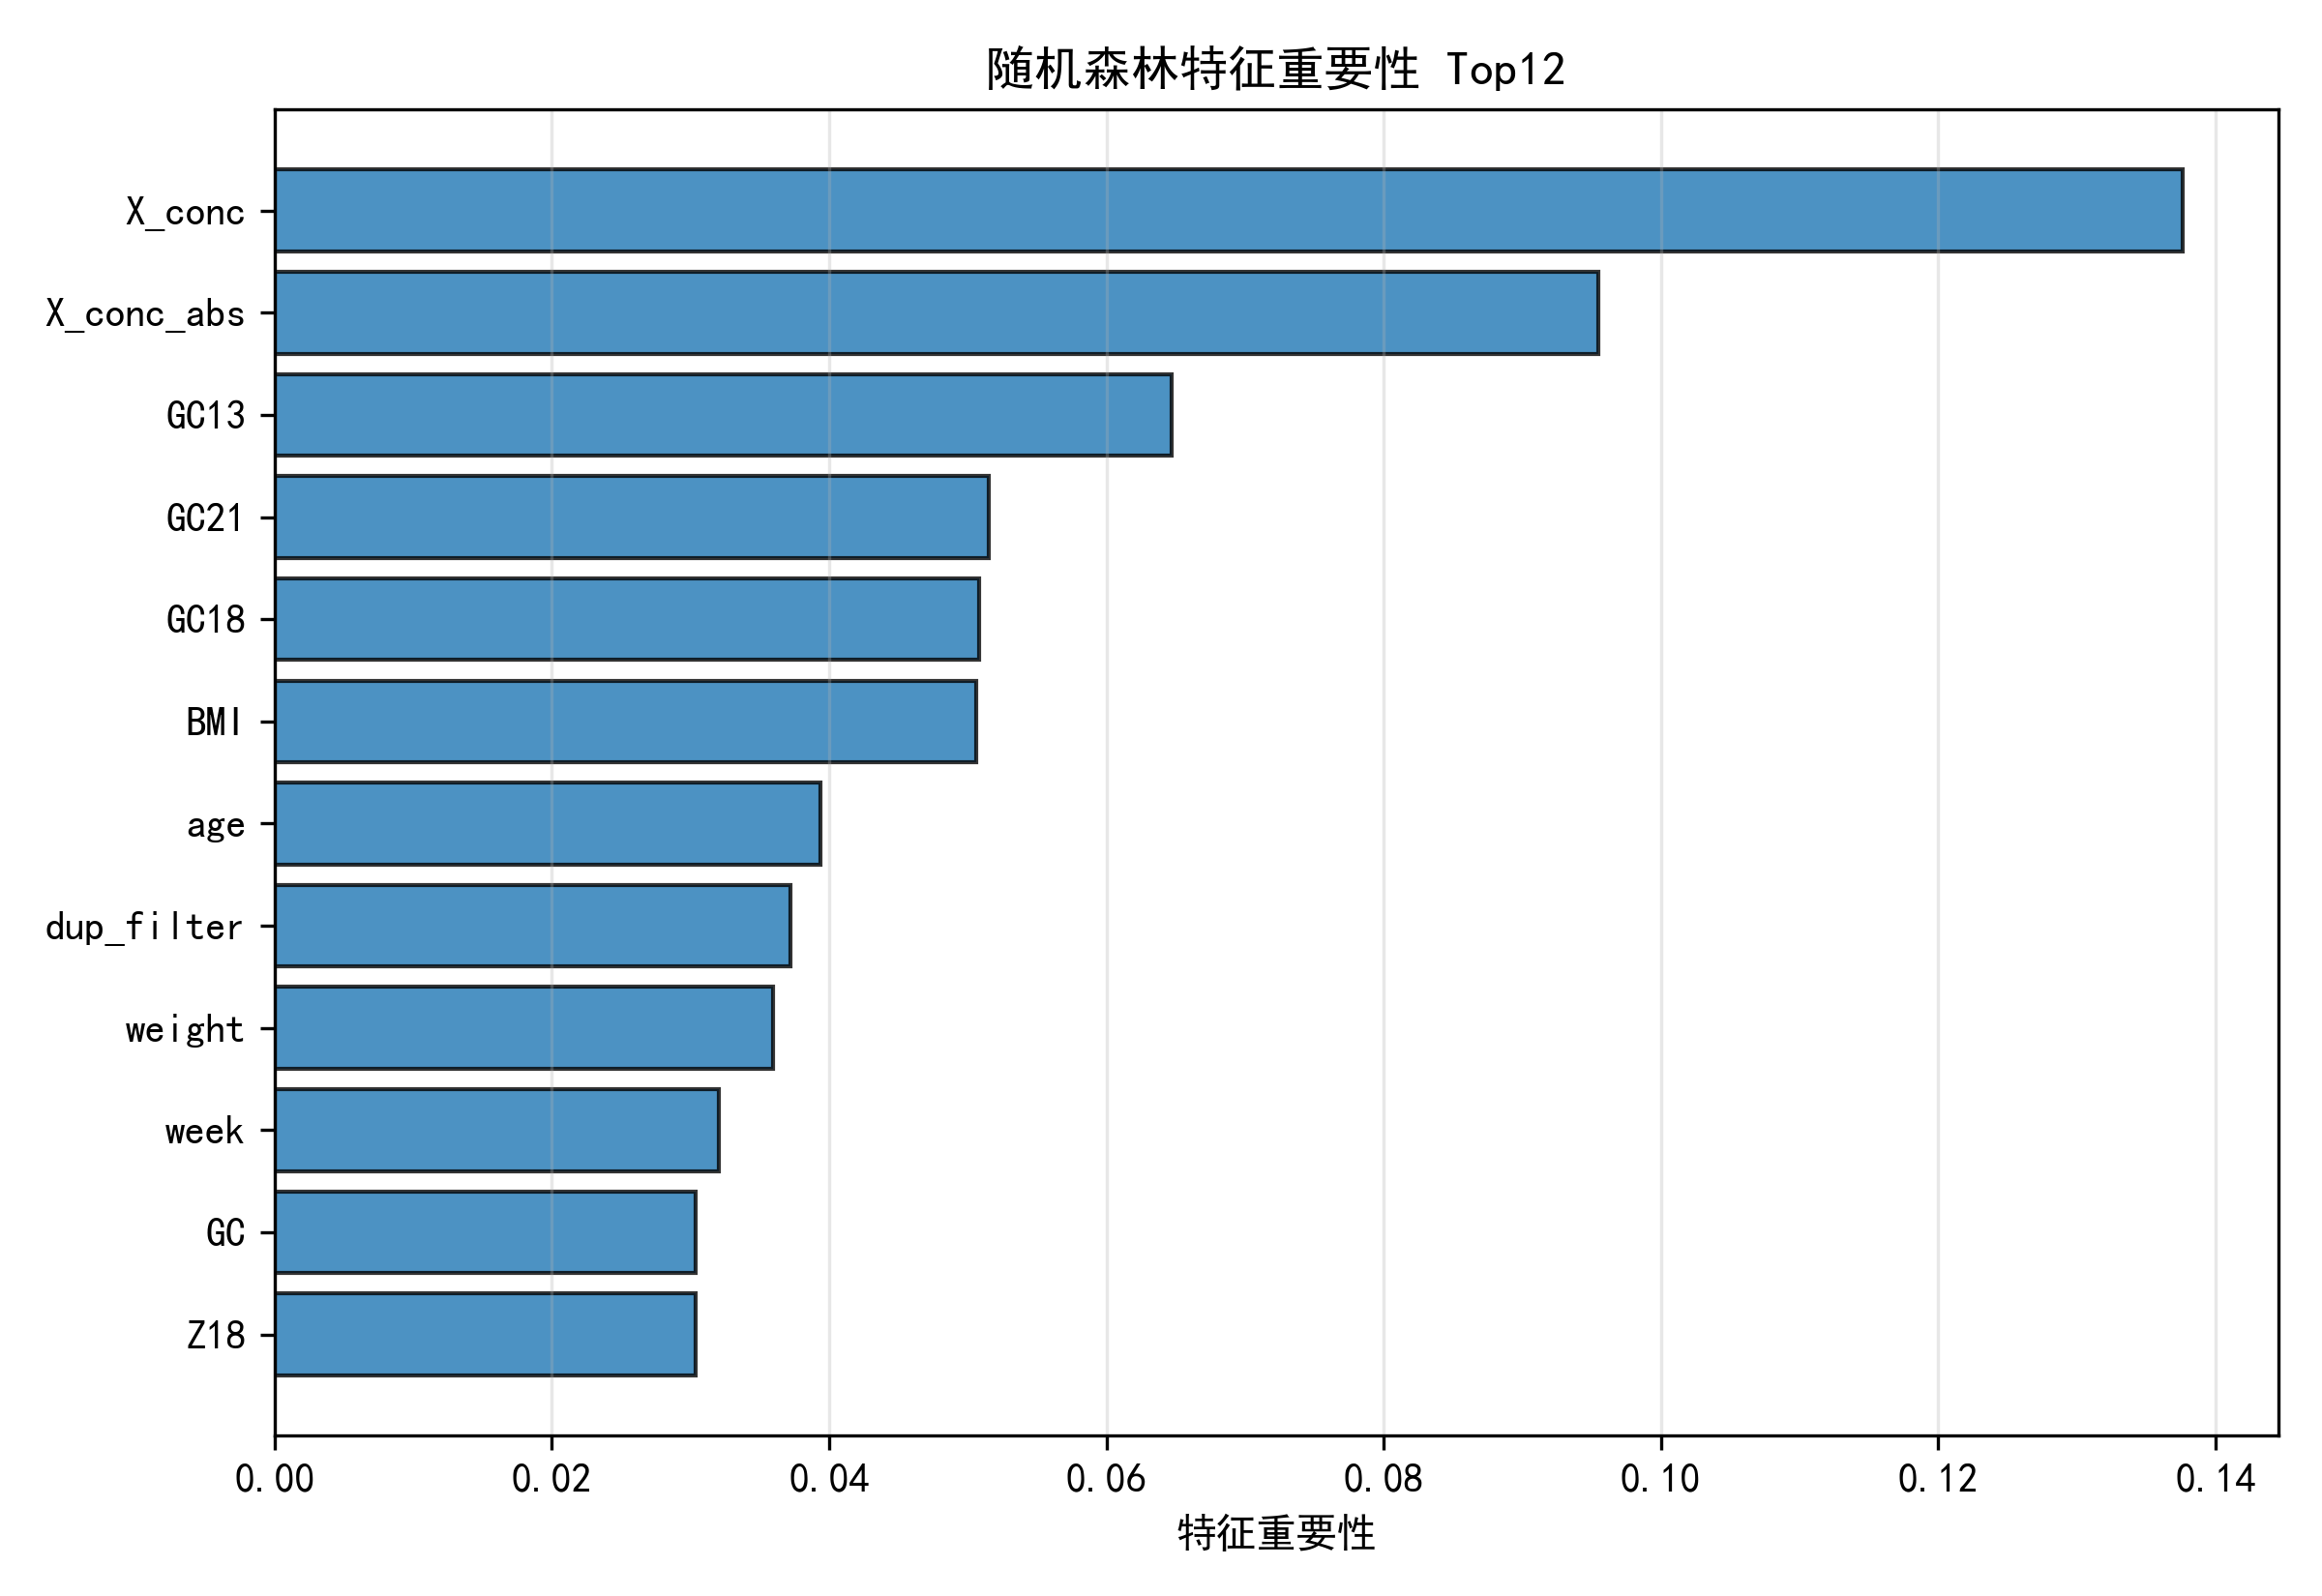
\includegraphics[width=0.8\textwidth]{output/figures/fig4-3_特征重要性.png}
\caption{随机森林特征重要性排序（前12位）}
\label{fig:p4imp}
\end{figure}

针对类别不平衡（异常仅占$11.1\%$），进一步对比了SMOTE过采样（在训练折内对少数类合成样本至平衡）与类别权重平衡两种处理方法，结果见表\ref{tab:smote}。二者AUC与敏感度相当（$0.795$ vs $0.794$），表明类别不平衡并非性能瓶颈；敏感度约$0.67$的上限源于异常样本的Z值未显著偏离正常（见图\ref{fig:zdist}），而非采样策略所致。鉴于类别权重平衡无需合成样本、可解释性更强，本文沿用该方法。

\begin{table}[H]
\centering
\caption{类别不平衡处理方法对比（逻辑回归，5折交叉验证）}
\label{tab:smote}
\begin{tabular}{lrrr}
\toprule
方法 & AUC & 敏感度 & 特异度 \\
\midrule
类别权重平衡 & 0.794 & 0.669 & 0.812 \\
SMOTE过采样 & 0.795 & 0.684 & 0.827 \\
\bottomrule
\end{tabular}
\end{table}

\subsection{可解释的判定公式}

尽管随机森林通过特征重要性揭示了X染色体浓度与GC含量的判别作用，但黑箱模型不利于临床落地。为此，本文进一步拟合标准化逻辑回归，给出可直接使用的线性判定公式。对特征做z-score标准化$X'_j=(X_j-\mu_j)/\sigma_j$后，异常概率的对数几率为
\begin{equation}
\log\frac{P}{1-P}=-0.846+\sum_{j}\beta_j X'_j,
\end{equation}
各特征系数（按$|\beta_j|$降序）见表\ref{tab:logreg}，其余14个特征系数绝对值均小于$0.18$，判别贡献有限。当$P>0.5$时判为异常，需进一步行羊水穿刺确诊。

\begin{table}[H]
\centering
\caption{标准化逻辑回归系数（前12位）}
\label{tab:logreg}
\begin{tabular}{lrrr}
\toprule
特征 & 系数$\beta_j$ & 均值$\mu_j$ & 标准差$\sigma_j$ \\
\midrule
21号染色体GC含量 & $-2.634$ & 0.4012 & 0.0050 \\
13号染色体GC含量 & 1.660 & 0.3791 & 0.0044 \\
18号染色体GC含量 & 1.101 & 0.3919 & 0.0042 \\
X染色体浓度 & $-0.587$ & $-0.0069$ & 0.0180 \\
$|$X染色体浓度$|$ & 0.469 & 0.0151 & 0.0119 \\
年龄（岁） & $-0.439$ & 30.018 & 4.305 \\
体重（kg） & $-0.317$ & 83.816 & 9.556 \\
孕周（周） & 0.273 & 18.346 & 4.366 \\
比对比例 & 0.269 & 0.7958 & 0.0177 \\
重复读段比例 & $-0.261$ & 0.0304 & 0.0034 \\
21号染色体Z值 & 0.256 & $-0.117$ & 1.124 \\
18号染色体Z值 & 0.188 & 0.804 & 1.283 \\
\bottomrule
\end{tabular}
\end{table}

由表\ref{tab:logreg}可见，三号染色体的GC含量标准化系数最大，这是因为GC含量的原始量纲极小（标准差约$0.005$），单位标准化变化即对应较大的几率偏移；X染色体浓度系数为$-0.587$，表明X浓度越低异常风险越高，与随机森林"X染色体浓度是最重要判别特征"的结论一致，也印证了题目"女胎以X染色体浓度判断检测可靠性"的临床经验。

\section{模型评价与改进}

\subsection{模型优点}
混合效应模型正确处理了纵向重复测量结构，避免了横截面回归对孕周效应的低估，这是本文方法上的核心改进。达标时间采用"真实达标"与"测得达标"的区分，将检测误差的影响显式量化。女胎判定综合多特征后AUC由阈值法的接近$0.5$提升至$0.79$，并识别出X染色体浓度的主导作用。

\subsection{模型局限与改进}
其一，达标时间的线性外推在数据范围（10--29周）外不可靠，本文仅在检测窗口内使用，未外推到10周以前。其二，女胎分类的AUC为$0.79$，仍有$33\%$的异常样本被逻辑回归漏判。43位孕妇的多次检测标签不一致引入了标签噪声，本文已测试孕妇级别的多数投票聚合，但AUC反而由$0.794$降至$0.733$，原因是样本量由605条缩至147条、且聚合放大了个别误报，故保留检测级别建模。其三，风险权衡通过置信水平$\alpha$体现，本文已对$\alpha$在$60\%\sim95\%$间扫描（见表\ref{tab:alpha}）验证了$80\%$选择的稳健性，但延误风险的三级离散设定（低/高/极高）仍可细化为连续函数；孕周二次项在决策窗口外推不可靠（见表\ref{tab:quad}），说明线性近似存在局限，未来可引入分段线性或样条模型。

\section{参考文献}

\begin{enumerate}[label={[\arabic*]}]
    \item Lo Y M D, Corbetta N, Chamberlain P F, et al. Presence of fetal DNA in maternal plasma and serum[J]. The Lancet, 1997, 350(9076): 485-487.
    \item Pinheiro J C, Bates D M. Mixed-Effects Models in S and S-PLUS[M]. New York: Springer, 2000.
    \item Breiman L. Random Forests[J]. Machine Learning, 2001, 45(1): 5-32.
    \item Hosmer D W, Lemeshow S. Applied Logistic Regression[M]. 2nd ed. New York: John Wiley \& Sons, 2000.
\end{enumerate}

\section*{附录：代码与结果文件说明}

本文全部计算由Python实现，依赖\texttt{numpy}、\texttt{pandas}、\texttt{statsmodels}、\texttt{scikit-learn}、\texttt{matplotlib}。代码文件分别为\texttt{problem1.py}至\texttt{problem4.py}，共享数据预处理模块\texttt{data\_utils.py}。所有图表输出于\texttt{output/figures/}，关键结果表输出于\texttt{output/}目录下的CSV文件。

\end{document}
